\bookmarksetup{bold,color=grass}
\chapter{绘图  pgf/tikz/pgfplot}
\bookmarksetup{bold=false,color={}}
\thispagestyle{fancy}
~\\[9cm]
\begin{flushright}
\kai\xiaosi
\textcolor[rgb]{0.00,0.50,0.00}{
毋意、毋必、毋固、毋我\\
- - 论语}
\end{flushright}
\clearpage
pgf 最大的优点是可以直接放在源码 tex 文件中,即可以编译预览,帅气的中文支持,可直接用 PDFLaTeX 和 \XeLaTeX 和文档一起编译(比 mp 和 asy 方便),无须另外设置,在图形环境里还可以同样调用 \LaTeX 命令(如 listings 等宏包很有用)。而且 pgf 作者为 beamer 包的作者 Till Tantau 可以很好地兼容 beamer 文件。下面为其应用手册简介。

由于本人是电子工程师,要画各种电路图,程序流程图,时序图。所以选择以下几个作重点介绍。

参考手册见\ref{texref}看效果吧:\\~\\

\begin{tikzpicture}
  [scale=3,line cap=round,
   % Styles
   axes/.style=,
   important line/.style={very thick},
   information text/.style={rounded corners,fill=red!10,inner sep=1ex}]

  % Local definitions
  \def\costhirty{0.8660256}

  % Colors
  \colorlet{anglecolor}{green!50!black}
  \colorlet{sincolor}{red}
  \colorlet{tancolor}{orange!80!black}
  \colorlet{coscolor}{blue}

  % The graphic
  \draw[help lines,step=0.5cm] (-1.4,-1.4) grid (1.4,1.4);

  \draw (0,0) circle (1cm);

  \begin{scope}[axes]
    \draw[->] (-1.5,0) -- (1.5,0) node[right] {$x$};
    \draw[->] (0,-1.5) -- (0,1.5) node[above] {$y$};

    \foreach \x/\xtext in {-1, -.5/-\frac{1}{2}, 1}
      \draw[xshift=\x cm] (0pt,1pt) -- (0pt,-1pt) node[below,fill=white] {$\xtext$};

    \foreach \y/\ytext in {-1, -.5/-\frac{1}{2}, .5/\frac{1}{2}, 1}
      \draw[yshift=\y cm] (1pt,0pt) -- (-1pt,0pt) node[left,fill=white] {$\ytext$};
  \end{scope}

  \filldraw[fill=green!20,draw=anglecolor] (0,0) -- (3mm,0pt) arc(0:30:3mm);
  \draw (15:2mm) node[anglecolor] {$\alpha$};

  \draw[important line,sincolor]
    (30:1cm) -- node[left=1pt,fill=white] {$\sin \alpha$} +(0,-.5);

  \draw[important line,coscolor]
    (0,0) -- node[below=2pt,fill=white] {$\cos \alpha$} (\costhirty,0);

  \draw[important line,tancolor] (1,0) --
    node [right=1pt,fill=white]
    {
      $\displaystyle \tan \alpha \color{black}=
      \frac{{\color{sincolor}\sin \alpha}}{\color{coscolor}\cos \alpha}$
    } (intersection of 0,0--30:1cm and 1,0--1,1) coordinate (t);

  \draw (0,0) -- (t);

  \draw[xshift=1.85cm] node [right,text width=6cm,information text]
    {
      The {\color{anglecolor} angle $\alpha$} is $30^\circ$ in the
      example ($\pi/6$ in radians). The {\color{sincolor}sine of
        $\alpha$}, which is the height of the red line, is
      \[
      {\color{sincolor} \sin \alpha} = 1/2.
      \]
      By the Theorem of Pythagoras we have ${\color{coscolor}\cos^2 \alpha} +
      {\color{sincolor}\sin^2\alpha} =1$. Thus the length of the blue
      line, which is the {\color{coscolor}cosine of $\alpha$}, must be
      \[
      {\color{coscolor}\cos\alpha} = \sqrt{1 - 1/4} = \textstyle
      \frac{1}{2} \sqrt 3.
      \]%
      This shows that {\color{tancolor}$\tan \alpha$}, which is the
      height of the orange line, is
      \[
      {\color{tancolor}\tan\alpha} = \frac{{\color{sincolor}\sin
          \alpha}}{\color{coscolor}\cos \alpha} = 1/\sqrt 3.
      \]%
    };
\end{tikzpicture}


%%%%%%%%%%%%%%%%  %%%%%%%%%%%%%%%%%%%%%%
\section{tikz 使用方法}
注: \XeLaTeX 下的 shading 和 spy 宏包有问题,不能产生效果。
\subsection{调用宏包}
\subsection{调用环境}
\subsection{tikzset 绘图预定义}
可提前设置好颜色等设置和调用以前的模板。
\begin{itemize}
  \item \verb|\tikzset{...}|:在导言区或绘图前加入
  \item \verb|\begin{tikzpicture}[...]|;在 [] 中加入
\end{itemize}
\section{tikz 基本绘图命令}
\begin{itemize}
  \item tikz 是基于坐标系的,原点在当前左下角
  \item 每条绘图命令以分号结束
  \item 默认长度为1cm,可加可不加,shift 等其他命令必须加.
\end{itemize}


\subsection{绘图环境和绘图命令}
绘图环境,tikz 绘图的基本单元是路径 path,路径有点和连接方式两种基本元素,可以被画、填充、裁剪...。
点可以通过坐标或其他方式给出,连接方式有直线、曲线、弧线。


\begin{minipage}[c]{9cm}
\begin{cmd}[label= Path 的绘制命令]
\path[draw](1,1)--(2,2)--(3,1);
\path[draw,yshift=-2cm]%
(1,1)--(2,2)--(3,1)--cycle;
\path[draw,fill=green!20,yshift=-4cm]%
(1,1)--(2,2)--(3,1)--cycle;
\path[fill=green,yshift=-6cm]%
(1,1)--(2,2)--(3,1)--cycle;
\path[clip,draw,yshift=-8cm]%
(1,1)--(2,2)--(3,1)--cycle;
\path[fill=blue!50](2,1.7-8)circle(.8);
\end{tikzpicture}
\end{cmd}
\end{minipage}
\quad\quad
\begin{minipage}{3cm}
\begin{tikzpicture}
\path[draw](1,1)--(2,2)--(3,1);
\path[draw,yshift=-2cm]%
(1,1)--(2,2)--(3,1)--cycle;
\path[draw,fill=green!20,yshift=-4cm]%
(1,1)--(2,2)--(3,1)--cycle;
\path[fill=green,yshift=-6cm]%
(1,1)--(2,2)--(3,1)--cycle;
\path[clip,draw,yshift=-8cm]%
(1,1)--(2,2)--(3,1)--cycle;
\path[fill=blue!50](2,1.7-8)circle(.8);
\end{tikzpicture}
\end{minipage}

\begin{cmd}[label= Path 的缩写命令]
\draw=\path[draw]
\fill=\path[fill]
\clip=\path[clip]
\filldraw=\path[fill,draw]
\shade=\path[shade]
\end{cmd}
\begin{itemize}
  \item \verb|\tikz|或\verb|\begin{tikzpicture}| 开始绘制环境
   \item \verb|\draw| 和\verb|\filldraw| 等直接绘制命令。
    \item \verb|\foreach|  等控制绘制命令。
\end{itemize}


\subsection{绘制路径}
\begin{minipage}{2.5cm}
\begin{tikzpicture}[thick]
\draw (0,3) -- (3,3);
\draw[decorate,decoration=zigzag] (0,2.5) -- (3,2.5);
\draw[decorate,decoration=brace] (0,2) -- (3,2);
\draw[decorate,decoration=triangles] (0,1.5) -- (3,1.5);
\draw[decorate,decoration={coil,segment length=4pt}] (0,1) -- (3,1);
\draw[decorate,decoration={coil,aspect=0}] (0,.5) -- (3,.5);
\draw[decorate,decoration={expanding waves,angle=7}] (0,0) -- (3,0);
\end{tikzpicture}
\end{minipage}
\begin{minipage}{10cm}
\begin{lstlisting}
\begin{tikzpicture}[thick]
\draw (0,3) -- (3,3);
\draw[decorate,decoration=zigzag] (0,2.5) -- (3,2.5);
\draw[decorate,decoration=brace] (0,2) -- (3,2);
\draw[decorate,decoration=triangles] (0,1.5) -- (3,1.5);
\draw[decorate,decoration={coil,segment length=4pt}] (0,1) -- (3,1);
\draw[decorate,decoration={coil,aspect=0}] (0,.5) -- (3,.5);
\draw[decorate,decoration={expanding waves,angle=7}] (0,0) -- (3,0);
\end{tikzpicture}
\end{lstlisting}
\end{minipage}

\subsection{绘制结点和标注 node coordinate}
\begin{cmd}[label= node 添加标注用法]
\draw (x1,y1)--(x2,y2) node[anchor=方向]{标注文字}
方向有 east,north,west,south
\node[选项]at(x,y)[选项]{text}
text 为显示的文字
\node(标记)[选项]at(x,y)[选项]{text}
\coordinate[label=角度:标注](标记)at(x,y)
\end{cmd}
\section{输出 pdf,png,eps单独格式图片}


\subsection{ pdf 图形全部预览 preview}
在导言区加入 preview 宏包,可实现全部 tikz 环境的图形预览,每个图形一页。包括 circuitikz 和 tikz-timing 宏包环境。可单独建立一个tex文件以实现单独的PDF文件输出,PreviewBorder 内的参数表示图形与周围空白的间距。
\begin{cmd}
\usepackage[active,tightpage]{preview}
\PreviewEnvironment{tikzpicture}
\setlength\PreviewBorder{15pt}
\end{cmd}

\subsection{xelatex 设置单独输出 pdf}
在 winedt 设置中将 options$\rightarrow$Execution Mode$\rightarrow$Console Applications$\rightarrow$\XeLaTeX$\rightarrow$Executable 的值变成如下所示,加入 -shell-escape 参数的作用是使 \XeLaTeX 能递归调用自己来产生图片。pdflatex 同上所示。
\begin{cmd}
  xelatex.exe -shell-escape
\end{cmd}
\subsection{调用宏包及设置}
需要tikz,tikzlibrary 的 extern 包。
\begin{lstlisting}[language={[LaTeX]TeX}]
\usepackage{tikz}
\usetikzlibrary{external}
\tikzexternalize %activate!
\tikzset{external/system call={xelatex \tikzexternalcheckshellescape
-halt-on-error-interaction=batchmode -jobname "\image" "\texsource"}}
\tikzsetexternalprefix{figures/}% 设置图片保存路径
\tikzsetnextfilename{trees} % 紧跟下一幅图名
\tikzsetfigurename{subset_} % 重设默认图名重设可用 {} 限定范围
\tikzexternaldisable % 暂时取消
\tikzexternalenable % 重新使能
\end{lstlisting}
\subsection{external 宏包兼容性设置}
如果 \XeLaTeX 调用了 \verb|\def\pgfsysdriver{pgfsys-dvipdfmx.def}| 命令,会导致出错不能使用 external,如果要用 pdfpage 等宏包,需在导言区做以下更改引用相关宏包。
\begin{lstlisting}[language={[LaTeX]TeX}]
\usetikzlibrary{external}
\tikzifexternalizing{%
%don'tincludepackageXYZhere
}{%
\usepackage{pdfpages}
\usepackage{vmargin}
...
}%
\end{lstlisting}

\section{插入外部图片}

\begin{enumerate}
  \item 声明 \verb|\pgfdeclareimage[options]{image name}{filename}|
  \item 插入 \verb|pgfuseimage{image name}|
  \item 或用以下命令替代上述两个命令 \verb|\pgfimage[options]{filename}|
\end{enumerate}


\section{结点样式 shapes decoration patterns shadows fadings backgrounds}

\subsection{shapes 形状}
基本的有圆和长方形: circle,rectangle。
扩展形状: geometric,symbol,arrow,multipart,callout,misc

shapes.geometric 有 diamond,ellipse,trapezium,semicircle,regular polygon,star,isosceles triangle,kite,dart,circular sector,cylinder。
\begin{tikzpicture}


\end{tikzpicture}



\section{结点关系 chains matrix tree automata fit}

\subsection{chains 链状图}

\begin{cmd}[label= pgf 链状图加载库]
  \usetikzlibrary{chains} % LATEX and plain TEX
\end{cmd}
链状图有很多种,可根据链的形状分成直线,曲线,分支线这几种,如下图所示:


\begin{minipage}{3cm}
\begin{tikzpicture}[start chain=going {at=(\tikzchainprevious),shift=(30:1)}]
\draw [help lines] (0,0) grid (3,2);
\node [draw,on chain] {1};
\node [draw,on chain] {Hello};
\node [draw,on chain] {World};
\node [draw,on chain] {.};
\end{tikzpicture}
\end{minipage}~~
\begin{minipage}{3cm}
\begin{tikzpicture}[start chain=circle placed {at=(\tikzchaincount*30:1.5)}]
\foreach \i in {1,...,10}
\node [on chain] {\i};
\draw (circle-1) -- (circle-10);
\end{tikzpicture}
\end{minipage}~~
\begin{minipage}{4cm}
\begin{tikzpicture}[every node/.style=draw]
\matrix [matrix of nodes,column sep=5mm,row sep=5mm]
{
|(a)| World & |(b) [circle]| peace \\
|(c)| be & |(d) [isosceles triangle]| would \\
|(e) [ellipse]| great & |(f)| ! \\
};
{ [start chain,every on chain/.style={join=by ->}]
\chainin (a);
\chainin (b);
\chainin (d);
\chainin (c);
\chainin (e);
\chainin (f);
}
\end{tikzpicture}
\end{minipage}~
\begin{minipage}{3cm}
  \begin{tikzpicture}[every on chain/.style=join,every join/.style=->,
node distance=2mm and 1cm]
{ [start chain=trunk]
\node [on chain] {A};
\node [on chain] {B};
{ [start branch=numbers going below]
\node [on chain] {1};
\node [on chain] {2};
\node [on chain] {3};
}
{ [start branch=greek going above]
\node [on chain] {$\alpha$};
\node [on chain] {$\beta$};
\node [on chain] {$\gamma$};
}
\node [on chain,join=with trunk/numbers-end,join=with trunk/greek-end] {C};
{ [start branch=symbols going below]
\node [on chain] {$\star$};
\node [on chain] {$\circ$};
\node [on chain] {$\int$};
}
}
\end{tikzpicture}
\end{minipage}

链状图绘制要点:
\begin{itemize}
  \item 链状图库是方便节点的放置而设计的,通过加载 chains 库可以方便地对一大堆元素进行位置的摆放
  \item 2
  \item 3
\end{itemize}

\subsection{matrix 矩阵图}

\begin{minipage}{3cm}
\begin{tikzpicture}
\matrix (magic) [matrix of nodes]
{
8 & 1 & 6 \\
3 & 5 & 7 \\
4 & 9 & 2 \\
};
\draw[thick,red,->] (magic-1-1) |- (magic-2-3);
\end{tikzpicture}

\begin{tikzpicture}
\matrix [matrix of nodes]
{
8 &[1cm] 1 &[3mm] |[red]| 6 \\
3 & 5 & |[red]| 7 \\
4 & 9 & 2 \\
};
\end{tikzpicture}

\begin{tikzpicture}
\matrix [matrix of math nodes,nodes={circle,draw},nodes in empty cells]
{
a_8 & & a_6 \\
a_3 & & a_7 \\
a_4 & a_9 & \\
};
\end{tikzpicture}
\end{minipage}
%%%%%%%%%%%%%%%%%%%%%%%%%%%%%%%%%%%
\begin{minipage}{10cm}
\scriptsize
\begin{lstlisting}
\begin{tikzpicture}
\matrix (magic) [matrix of nodes]
{
8 & 1 & 6 \\
3 & 5 & 7 \\
4 & 9 & 2 \\
};
\draw[thick,red,->] (magic-1-1) |- (magic-2-3);
\end{tikzpicture}

\begin{tikzpicture}
\matrix [matrix of nodes]
{
8 &[1cm] 1 &[3mm] |[red]| 6 \\
3 & 5 & |[red]| 7 \\
4 & 9 & 2 \\
};
\end{tikzpicture}

\begin{tikzpicture}
\matrix
[matrix of math nodes,nodes={circle,draw},nodes in empty cells]
{
a_8 & & a_6 \\
a_3 & & a_7 \\
a_4 & a_9 & \\
};
\end{tikzpicture}
\end{lstlisting}
\end{minipage}


\subsection{tree qtree树状图}


\begin{minipage}{3cm}

%\tikzsetnextfilename{trees}
\begin{tikzpicture}
[edge from parent fork down,
every node/.style={fill=red!30,rounded corners},
edge from parent/.style={red,-o,thick,draw}]
\node {root}
child {node {left}}
child {node {right}
child {node {child}}
child {node {child}}
};
\end{tikzpicture}
\end{minipage}
\begin{minipage}{11cm}
\begin{lstlisting}
\begin{tikzpicture}
[edge from parent fork down,
every node/.style={fill=red!30,rounded corners},
edge from parent/.style={red,-o,thick,draw}]
\node {root}
child {node {left}}
child {node {right}
child {node {child}}
child {node {child}}
};
\end{tikzpicture}
\end{lstlisting}
\end{minipage}

树参数设置
\begin{description}
  \item[node] 结点形状
  \item[edge from parent] 结点连线
  \item[edge from parent fork down] down 可改为 left,right,up
  \item[grow] 结点增长方向
  \item[anchor] 结点连接处
  \item[level distance] node 和 child 间距
  \item[sibling distance] child 和 child 间距
  \item[sibling angle] 在 grow cyclic 方式下的角度
  \item[clockwise from] 第一个 child 的方向
  \item[grow via three points] 设定 edge 的增长方向角度 = one child at(x)and two children at(y) and (z)
\end{description}


\textbf{qtree 宏包设置},qtree 宏包是一个简化 tree 绘制的代码宏包,引入后可用简单的代码来实现树的绘制。


\begin{minipage}{6.5cm}
\begin{tikzpicture}
\tikzset{level distance=60pt,every node/.style={fill=red!30,rounded corners},}
\Tree [.NP [.Adj tall ] [.N tree ] ]
\end{tikzpicture}
\begin{tikzpicture}[sibling distance=72pt]
\Tree [.NP [.Adj fat ] [.N tree ] ]
\end{tikzpicture}
\end{minipage}
\begin{minipage}{11cm}
\begin{lstlisting}
\begin{tikzpicture}
\tikzset{level distance=60pt,
every node/.style={fill=red!30,rounded corners},}
\Tree [.NP [.Adj tall ] [.N tree ] ]
\end{tikzpicture}
%
\begin{tikzpicture}[sibling distance=72pt]
\Tree [.NP [.Adj fat ] [.N tree ] ]
\end{tikzpicture}
\end{lstlisting}
\end{minipage}
\subsection{automata 状态机}

\noindent 绘制状态机可通过以下几个步骤进行:
\begin{description}
  \item[1. tikzpicture 参数设置:]设置结点,箭头和文字参数,包括颜色,方向,大小形状等;
  \item[2. 绘制背景:]画出网格等背景图形;
  \item[3. node 参数设置:]摆放结点位置;
  \item[4. path 参数设置:]设置连接线及标注。
\end{description}

\begin{minipage}{5cm}
\begin{tikzpicture}[shorten >=1pt,node distance=2cm,on grid,auto]
\draw[help lines] (0,0) grid (3,2);
\node[state,initial] (q_0) {$q_0$};
\node[state] (q_1) [above right=of q_0] {$q_1$};
\node[state] (q_2) [below right=of q_0] {$q_2$};
\node[state,accepting](q_3) [below right=of q_1] {$q_3$};
\path[->] (q_0) edge node {0} (q_1)
edge node [swap] {1} (q_2)
(q_1) edge node {1} (q_3)
edge [loop above] node {0} ()
(q_2) edge node [swap] {0} (q_3)
edge [loop below] node {1} ();
\end{tikzpicture}
\end{minipage}
\begin{minipage}{10cm}
\begin{lstlisting}
\begin{tikzpicture}
[shorten >=1pt,node distance=2cm,on grid,auto]
\draw[help lines] (0,0) grid (3,2);
\node[state,initial] (q_0) {$q_0$};
\node[state] (q_1) [above right=of q_0] {$q_1$};
\node[state] (q_2) [below right=of q_0] {$q_2$};
\node[state,accepting](q_3) [below right=of q_1] {$q_3$};
\path[->] (q_0) edge node {0} (q_1)
edge node [swap] {1} (q_2)
(q_1) edge node {1} (q_3)
edge [loop above] node {0} ()
(q_2) edge node [swap] {0} (q_3)
edge [loop below] node {1} ();
\end{tikzpicture}
\end{lstlisting}
\end{minipage}

\begin{tikzpicture}[->,>=stealth',shorten >=1pt,auto,node distance=2.8cm,on grid,semithick,
                    every state/.style={fill=red,draw=none,circular drop shadow,text=white}]

  \node[initial,state] (A)                    {$q_a$};
  \node[state]         (B) [above right=of A] {$q_b$};
  \node[state]         (D) [below right=of A] {$q_d$};
  \node[state]         (C) [below right=of B] {$q_c$};
  \node[state]         (E) [below=of D]       {$q_e$};

  \path (A) edge              node {0,1,L} (B)
            edge              node {1,1,R} (C)
        (B) edge [loop above] node {1,1,L} (B)
            edge              node {0,1,L} (C)
        (C) edge              node {0,1,L} (D)
            edge [bend left]  node {1,0,R} (E)
        (D) edge [loop below] node {1,1,R} (D)
            edge              node {0,1,R} (A)
        (E) edge [bend left]  node {1,0,R} (A);

   \node [right=0.2cm,text width=10cm] at (C)
   {\scriptsize
\begin{lstlisting}[language={verilog},backgroundcolor={\color{red!10}}]
\begin{tikzpicture}
[->,>=stealth',shorten >=1pt,auto,
node distance=2.8cm,on grid,semithick,
every state/.style={fill=red,draw=none,
circular drop shadow,text=white}]
  \node[initial,state] (A)                    {$q_a$};
  \node[state]         (B) [above right=of A] {$q_b$};
  \node[state]         (D) [below right=of A] {$q_d$};
  \node[state]         (C) [below right=of B] {$q_c$};
  \node[state]         (E) [below=of D]       {$q_e$};

  \path (A) edge              node {0,1,L} (B)
            edge              node {1,1,R} (C)
        (B) edge [loop above] node {1,1,L} (B)
            edge              node {0,1,L} (C)
        (C) edge              node {0,1,L} (D)
            edge [bend left]  node {1,0,R} (E)
        (D) edge [loop below] node {1,1,R} (D)
            edge              node {0,1,R} (A)
        (E) edge [bend left]  node {1,0,R} (A);
\end{tikzpicture}
\end{lstlisting}
   };
\end{tikzpicture}

\subsection{pgf 流程图}

设置好结点和图形,放在导言区。
\begin{lstlisting}
\tikzset{
passprocess/.style={
rectangle,
draw=blue,
minimum width=50pt,
minimum height=20pt,
font=\ttfamily,
text centered
},
startstop/.style={
rectangle,%
rounded corners=5pt,%
minimum width=50pt,
minimum height=20pt,
text centered,
fill=orange,
font=\ttfamily,
draw=red
},
decision/.style={
diamond,%
shape aspect=2,%aspect value is the ratio of width and height for diamond
draw=green,%the color of line
fill=lime,%filled color
font=\ttfamily,%set font
text centered%surely you know what it means
},%here is a
line/.style = {
draw,
->,
%shorten>=2pt,
thick
}}
\end{lstlisting}


\begin{cmd}[label=流程图命令]
\matrix [row sep=行距,column sep=列距]{节点定义代码} %节点行列分布
\node (节点序号) [节点类型] {节点内容} %节点内容设置
\begin{scope}[every path/.style=line] %节点连线设置
\path () -- () %竖线相连
\path () |- () %先竖再折
\path () -| () %先折再竖
\end{scope}
\end{cmd}

\begin{tikzpicture}
\matrix[row sep=5mm,column sep=5mm]
{
%First row:
\node (p1) [startstop] {开始};&\\
%Second row;
\node (p2) [passprocess] {问问题咯};&\\
%Third row:
\node (p31) [decision] {a你是大牛么:?};&
\node (p32) [passprocess] {b你才是大牛:};\\
%Fourth row:
&
\node (p4) [passprocess] {b你全家都是大牛:};\\
%Fifth row:
&
\node (p42) [passprocess] {b你家小狗都是大牛:};\\
%Sixth row:
\node (p5) [passprocess] {a当我什么也没说:};&\\
%Seventh row:
\node (p6) [startstop] {结束};&\\
};

\begin{scope}[every path/.style=line]
\path (p1) -- (p2);
\path (p2) -- (p31);
\path (p31) -- node [near start,above] {yes} (p32);
\path (p32) -- (p4);
\path (p4) -- (p42);
\path (p5) -- (p6);
\path (p42) |-(p5);%表示先竖后折, -|表示先折后竖
\path (p31) -- node [midway,left] {no} (p5);
\end{scope};
\draw[xshift=4.35cm] node [right,text width=7cm,information text]
    {\tiny
    \begin{lstlisting}[backgroundcolor={\color{red!10}}]
\begin{tikzpicture}
[information text/.style={rounded corners,
fill=red!10,inner sep=0ex}]
\matrix[row sep=5mm,column sep=5mm]
{
%First row:
\node (p1) [startstop] {`开始`};&\\
%Second row;
\node (p2) [passprocess] {`问问题咯`};&\\
%Third row:
\node (p31) [decision] {a`你是大牛么`:?};&
\node (p32) [passprocess] {b`你才是大牛`:};\\
%Fourth row:
&
\node (p4) [passprocess] {b`你全家都是大牛`:};\\
%Fifth row:
&
\node (p42) [passprocess] {b`你家小狗都是大牛`:};\\
%Sixth row:
\node (p5) [passprocess] {a`当我什么也没说`:};&\\
%Seventh row:
\node (p6) [startstop] {`结束`};&\\
};

\begin{scope}[every path/.style=line]
\path (p1) -- (p2);
\path (p2) -- (p31);
\path (p31) -- node [near start,above] {yes} (p32);
\path (p32) -- (p4);
\path (p4) -- (p42);
\path (p5) -- (p6);
\path (p42) |-(p5);%`表示先竖后折, -|表示先折后竖`
\path (p31) -- node [midway,left] {no} (p5);
\end{scope};
};
\end{tikzpicture}
    \end{lstlisting}
      };
\end{tikzpicture}



\subsection{pgfplot 坐标图}

\begin{tikzpicture}
[every entity/.style={draw=blue!50,fill=blue!20,thick}]
\node[entity] (sheep) {Sheep};
\node[entity] (genome) [right=of sheep] {Genome};
\end{tikzpicture}

\begin{tikzpicture}
\begin{axis}[
xlabel=Cost,
ylabel=Error]
\addplot[color=red,mark=x] coordinates {
(2,-2.8559703)
(3,-3.5301677)
(4,-4.3050655)
(5,-5.1413136)
(6,-6.0322865)
(7,-6.9675052)
(8,-7.9377747)
};
\end{axis}
\end{tikzpicture}




\section{pgf 日历图}


\begin{minipage}{4.5cm}
\tikz [every day/.style={anchor=mid}]
\calendar
[dates=2000-01-01 to 2000-01-31,week list]
if (Sunday) [red]
if (equals=2000-01-20) {\draw (0,0) circle (8pt);};
\end{minipage}
\begin{minipage}[b]{10cm}
\begin{lstlisting}
\tikz [every day/.style={anchor=mid}]
\calendar
[dates=2000-01-01 to 2000-01-31,week list]
if (Sunday) [red]
if (equals=2000-01-20) {\draw (0,0) circle (8pt);};
\end{lstlisting}
\end{minipage}


\begin{minipage}{4.5cm}
\begin{tikzpicture}
\calendar
[
dates=\year-\month-\day+-25 to \year-\month-\day+25,
week list,inner sep=2pt,month label above centered,
month text=\textit{\%mt \%y0}
]
if (at least=\year-\month-\day) {}
else [nodes={strike out,draw}]
if (at most=\year-\month-\day+7)
[green!50!black]
if (between=\year-\month-\day+8 and \year-\month-\day+10)
[red]
if (Sunday)
[gray,nodes={draw=none}]
;
\end{tikzpicture}
\end{minipage}
\begin{minipage}[c]{10cm}
\footnotesize
\begin{lstlisting}
\begin{tikzpicture}
\calendar
[
dates=\year-\month-\day+-25 to \year-\month-\day+25,
week list,inner sep=2pt,month label above centered,
month text=\textit{\%mt \%y0}
]
if (at least=\year-\month-\day) {}
else [nodes={strike out,draw}]
if (at most=\year-\month-\day+7)
[green!50!black]
if (between=\year-\month-\day+8 and \year-\month-\day+10)
[red]
if (Sunday)
[gray,nodes={draw=none}]
;
\end{tikzpicture}
\end{lstlisting}
\end{minipage}


\begin{minipage}{4.5cm}
\tikz
\calendar [dates=2000-01-20 to 2000-02-10,
week list,month label above right];
\end{minipage}
\begin{minipage}[b]{10cm}
\begin{lstlisting}
\tikz
\calendar [dates=2000-01-20 to 2000-02-10,
week list,month label above right];
\end{lstlisting}
\end{minipage}


\begin{minipage}{4.5cm}
\begin{tikzpicture}
\small\sffamily
\colorlet{darkgreen}{green!50!black}
\calendar[dates=\year-01-01 to \year-3-31,week list,
month label left,month yshift=0pt,
month text=\textcolor{darkgreen}{\%m0}]
if (Sunday) [black!50];
\end{tikzpicture}
\end{minipage}
\begin{minipage}[b]{10cm}
\begin{lstlisting}
\begin{tikzpicture}
\small\sffamily
\colorlet{darkgreen}{green!50!black}
\calendar[dates=\year-01-01 to \year-3-31,week list,
month label left,month yshift=0pt,
month text=\textcolor{darkgreen}{\%m0}]
if (Sunday) [black!50];
\end{tikzpicture}
\end{lstlisting}
\end{minipage}

\begin{cal}
\sffamily
\colorlet{winter}{blue}
\colorlet{spring}{green!60!black}
\colorlet{summer}{orange}
\colorlet{fall}{red}
% A counter, since TikZ is not clever enough (yet) to handle
% arbitrary angle systems.
\newcount\mycount
\begin{tikzpicture}
[transform shape,
every day/.style={anchor=mid,font=\fontsize{6}{6}\selectfont}]
\node{\normalsize\the\year};
\foreach \month/\monthcolor in
{1/winter,2/winter,3/spring,4/spring,5/spring,6/summer,
7/summer,8/summer,9/fall,10/fall,11/fall,12/winter}
{
% Computer angle:
\mycount=\month
\advance\mycount by -1
\multiply\mycount by 30
\advance\mycount by -90
% The actual calendar
\calendar at (\the\mycount:6.4cm)
[
dates=\the\year-\month-01 to \the\year-\month-last,
]
if (day of month=1) {\color{\monthcolor}\tikzmonthcode}
if (Sunday) [red]
if (all)
{
% Again, compute angle
\mycount=1
\advance\mycount by -\pgfcalendarcurrentday
\multiply\mycount by 11
\advance\mycount by 90
\pgftransformshift{\pgfpointpolar{\mycount}{1.4cm}}
};
}
\end{tikzpicture}
\begin{lstlisting}
\sffamily
\colorlet{winter}{blue}
\colorlet{spring}{green!60!black}
\colorlet{summer}{orange}
\colorlet{fall}{red}
% A counter, since TikZ is not clever enough (yet) to handle
% arbitrary angle systems.
\newcount\mycount
\begin{tikzpicture}
[transform shape,
every day/.style={anchor=mid,font=\fontsize{6}{6}\selectfont}]
\node{\normalsize\the\year};
\foreach \month/\monthcolor in
{1/winter,2/winter,3/spring,4/spring,5/spring,6/summer,
7/summer,8/summer,9/fall,10/fall,11/fall,12/winter}
{
% Computer angle:
\mycount=\month
\advance\mycount by -1
\multiply\mycount by 30
\advance\mycount by -90
% The actual calendar
\calendar at (\the\mycount:6.4cm)
[
dates=\the\year-\month-01 to \the\year-\month-last,
]
if (day of month=1) {\color{\monthcolor}\tikzmonthcode}
if (Sunday) [red]
if (all)
{
% Again, compute angle
\mycount=1
\advance\mycount by -\pgfcalendarcurrentday
\multiply\mycount by 11
\advance\mycount by 90
\pgftransformshift{\pgfpointpolar{\mycount}{1.4cm}}
};
}
\end{tikzpicture}
\end{lstlisting}

\end{cal}



\section{pgf spy 局部放大}

\begin{minipage}{3cm}
\begin{tikzpicture}
[spy using outlines={circle, magnification=4, size=2cm, connect spies}]
\draw [help lines] (0,0) grid (3,2);
\draw [decoration=Koch curve type 1]
decorate { decorate{ decorate{ decorate{ (0,0) -- (2,0) }}}};
\spy [red] on (1.6,0.3)
in node [left] at (3.5,-1.25);
\spy [blue, size=1cm] on (1,1)
in node [right] at (0,-1.25);
\end{tikzpicture}
\end{minipage}
\begin{minipage}{12cm}
\begin{lstlisting}
\begin{tikzpicture}
[spy using outlines=
{circle, magnification=4, size=2cm, connect spies}]
\draw [help lines] (0,0) grid (3,2);
\draw [decoration=Koch curve type 1]
decorate { decorate{ decorate
{ decorate{ (0,0) -- (2,0) }}}};
\spy [red] on (1.6,0.3)
in node [left] at (3.5,-1.25);
\spy [blue, size=1cm] on (1,1)
in node [right] at (0,-1.25);
\end{tikzpicture}
\end{lstlisting}
\end{minipage}


\section{动画设计}

  \newcommand{\mainaxis}{
        % Main axis
        \draw (-2, 0) -- (2, 0) (0, 0) -- (0, 1.15);

        % Small tickmarks on the x axis
        \foreach \x in {-2,-1.9,...,2} {
            \draw (\x, 0) -- (\x, -0.8pt);
        }

        % Labels on the $x$ axis; the llap makes the label center on the
        % number without the minus.
        \foreach \x/\label in {-2/\llap{$-$}2,-1/\llap{$-$}1,0/0,1/1,2/2} {
            \node[x tick label] at (\x, 0) {$\label$};
            \draw[major tick] (\x, 0) -- (\x, -1.25pt);
        }

        % Y tick mark.
        \draw[major tick] (-1.25pt,.5) -- (0,.5);

        % Y labels.
        \node[y tick label] at (0,.5) {$\frac{1}{2}$};
        \node[y tick label] at (0,1) {$1$};
    }

    \def\yshift{-2cm} % Shift of the lower axis
    \newcommand{\drawaxes}{
        \mainaxis
        \node[axis label] at (2,0) {$\scriptstyle \tau$};

        % Second axis, where the convultion will be drawn.
        \begin{scope}[yshift=\yshift]
            \foreach \y in {0.1,0.2,...,1.0}
                \draw[black!20] (-2,\y) -- (2,\y);
            \mainaxis
            \node[axis label] at (2,0) {$\scriptstyle t$};
        \end{scope}

        \begin{pgfonlayer}{foreground}
            \node at (0,1.25) {$f$};
            \node[anchor=base] at (0,-.55)
                {$f*g =\!\!\displaystyle\int\limits_{-\infty}^{\infty}
                    \!\!f(\tau)g(t-\tau)\,d\tau$};
        \end{pgfonlayer}

        \draw[major tick] (-1.25pt,.5) -- (0,.5) (-1.25pt,1) -- (0,1);

        % f(\tau) is basically fixed.
        \draw[function f] (-0.5, 0) -- +(0,1) -- +(1,1) -- +(1,0);
        \clip (-2,-2) rectangle (2, 1.75);
    }

    \newcommand{\drawg}[1]{
        \draw[function g] (#1,0) ++(-0.5, 0) -- +(0,1) -- +(1,1) -- +(1,0);
        \draw[function g position] (#1,1.4) -- (#1,\yshift);
        \node[fill=white] at (#1, 1.25) {$g$};

        % We now slightly abuse \ifdim to determine whether
        % there is an overlap.
        \ifdim#1pt>-1pt\ifdim#1pt<1.01pt
            % Draw legend.
            \fill[overlap] (-2,1.51) rectangle +(0.15,0.15);
            % The right side of f overlaps with the left side of g:
            % 'entering'
            \ifdim#1pt<0pt
                \node[anchor=west] at (-1.85, 1.575)
                    {$f(\tau)g(\pgfmathprintnumber{#1} - \tau$)};
                \begin{pgfonlayer}{background}
                    \fill[overlap] (-.5,0) rectangle (#1+.5,1);
                \end{pgfonlayer}
                \draw[convolution] (-1,\yshift) -- (#1, \yshift+1cm+#1 cm);
            \else
                % The left side of f overlaps with the right side of g:
                % 'leaving'
                \node[anchor=west] at (-1.85, 1.575)
                    {$f(\tau)g(\pgfmathprintnumber{#1} - \tau$)};
                \begin{pgfonlayer}{background}
                    \fill[overlap] (#1-.5,0) rectangle (.5,1);
                \end{pgfonlayer}
                \draw[convolution] (-1,\yshift) -- +(1, 1) --
                    (#1,\yshift+1cm-#1 cm);
            \fi
        \else
            % 'g' is completely past 'f', draw the result.
            \draw[convolution] (-1,\yshift) -- +(1,1) -- +(2,0);
        \fi\fi
    }

    \begin{animateinline}[controls,
        autoplay,buttonsize=1.2em,
        buttonbg=0.6:0.6:1,buttonfg=0.2:0.2:1,
        begin={\begin{tikzpicture}[scale=2]\drawaxes},
        end={\end{tikzpicture}}]{8}

        % Generate frames for -2 ... 2
        \xdef\pos{-2}
        \whiledo{\lengthtest{\pos pt < 2.1 pt}}{
            \drawg{\pos}\newframe
            \pgfmathsetmacro{\pos}{\pos + 0.1}
            \xdef\pos{\pos}
        }

        \drawg{\pos}
    \end{animateinline}

\scriptsize
\begin{lstlisting}
    \newcommand{\mainaxis}{
        % Main axis
        \draw (-2, 0) -- (2, 0) (0, 0) -- (0, 1.15);

        % Small tickmarks on the x axis
        \foreach \x in {-2,-1.9,...,2} {
            \draw (\x, 0) -- (\x, -0.8pt);
        }

        % Labels on the $x$ axis; the llap makes the label center on the
        % number without the minus.
        \foreach \x/\label in {-2/\llap{$-$}2,-1/\llap{$-$}1,0/0,1/1,2/2} {
            \node[x tick label] at (\x, 0) {$\label$};
            \draw[major tick] (\x, 0) -- (\x, -1.25pt);
        }

        % Y tick mark.
        \draw[major tick] (-1.25pt,.5) -- (0,.5);

        % Y labels.
        \node[y tick label] at (0,.5) {$\frac{1}{2}$};
        \node[y tick label] at (0,1) {$1$};
    }

    \def\yshift{-2cm} % Shift of the lower axis
    \newcommand{\drawaxes}{
        \mainaxis
        \node[axis label] at (2,0) {$\scriptstyle \tau$};

        % Second axis, where the convultion will be drawn.
        \begin{scope}[yshift=\yshift]
            \foreach \y in {0.1,0.2,...,1.0}
                \draw[black!20] (-2,\y) -- (2,\y);
            \mainaxis
            \node[axis label] at (2,0) {$\scriptstyle t$};
        \end{scope}

        \begin{pgfonlayer}{foreground}
            \node at (0,1.25) {$f$};
            \node[anchor=base] at (0,-.55)
                {$f*g =\!\!\displaystyle\int\limits_{-\infty}^{\infty}
                    \!\!f(\tau)g(t-\tau)\,d\tau$};
        \end{pgfonlayer}

        \draw[major tick] (-1.25pt,.5) -- (0,.5) (-1.25pt,1) -- (0,1);

        % f(\tau) is basically fixed.
        \draw[function f] (-0.5, 0) -- +(0,1) -- +(1,1) -- +(1,0);
        \clip (-2,-2) rectangle (2, 1.75);
    }

    \newcommand{\drawg}[1]{
        \draw[function g] (#1,0) ++(-0.5, 0) -- +(0,1) -- +(1,1) -- +(1,0);
        \draw[function g position] (#1,1.4) -- (#1,\yshift);
        \node[fill=white] at (#1, 1.25) {$g$};

        % We now slightly abuse \ifdim to determine whether
        % there is an overlap.
        \ifdim#1pt>-1pt\ifdim#1pt<1.01pt
            % Draw legend.
            \fill[overlap] (-2,1.51) rectangle +(0.15,0.15);
            % The right side of f overlaps with the left side of g:
            % 'entering'
            \ifdim#1pt<0pt
                \node[anchor=west] at (-1.85, 1.575)
                    {$f(\tau)g(\pgfmathprintnumber{#1} - \tau$)};
                \begin{pgfonlayer}{background}
                    \fill[overlap] (-.5,0) rectangle (#1+.5,1);
                \end{pgfonlayer}
                \draw[convolution] (-1,\yshift) -- (#1, \yshift+1cm+#1 cm);
            \else
                % The left side of f overlaps with the right side of g:
                % 'leaving'
                \node[anchor=west] at (-1.85, 1.575)
                    {$f(\tau)g(\pgfmathprintnumber{#1} - \tau$)};
                \begin{pgfonlayer}{background}
                    \fill[overlap] (#1-.5,0) rectangle (.5,1);
                \end{pgfonlayer}
                \draw[convolution] (-1,\yshift) -- +(1, 1) --
                    (#1,\yshift+1cm-#1 cm);
            \fi
        \else
            % 'g' is completely past 'f', draw the result.
            \draw[convolution] (-1,\yshift) -- +(1,1) -- +(2,0);
        \fi\fi
    }

    \begin{animateinline}[controls,
        autoplay,buttonsize=1.2em,
        buttonbg=0.6:0.6:1,buttonfg=0.2:0.2:1,
        begin={\begin{tikzpicture}[scale=2]\drawaxes},
        end={\end{tikzpicture}}]{8}

        % Generate frames for -2 ... 2
        \xdef\pos{-2}
        \whiledo{\lengthtest{\pos pt < 2.1 pt}}{
            \drawg{\pos}\newframe
            \pgfmathsetmacro{\pos}{\pos + 0.1}
            \xdef\pos{\pos}
        }

        \drawg{\pos}
    \end{animateinline}
\end{lstlisting}
\normalsize

\section{边注便笺}
给边注加一个便笺框。
\yellownote{设计备注:默认大小在导言设置}
\resizeyellownote{2}{1}{更改框大小使用命令}
\begin{cmd}[label=使用方法]
\yellownote{设计备注:默认大小在导言设置}
\resizeyellownote{2}{1}{设计备注:更改框大小使用命令}
\end{cmd}
在导言区得加入以下设置:
\footnotesize
\begin{lstlisting}
\newlength{\yellownotewidth}
\setlength{\yellownotewidth}{2cm}
\newlength{\yellownoteheight}
\setlength{\yellownoteheight}{2cm}
\newcommand{\yellownote}[1]{
\marginpar{
    \vspace{-0.5\yellownoteheight}
        \begin{center}
        \begin{tikzpicture}
            \draw[white,fill=gray!25,opacity=0.75,shift={(-0.125,-0.125)}]
                (0,0) rectangle (\yellownotewidth,\yellownoteheight);
            \draw[fill=yellow!35] (0,0) rectangle (\yellownotewidth,\yellownoteheight);
            \draw[opacity=0.45,fill=gray!50] (0.7\yellownotewidth,0) --
                (0.9\yellownotewidth,0.45) -- (\yellownotewidth,0.4) -- cycle;
            \node[blue,below] at (0.5\yellownotewidth,\yellownoteheight) {
                \begin{minipage}{\yellownotewidth-1em}
                    \scriptsize\sf#1
                \end{minipage}
            };
        \end{tikzpicture}
        \end{center}
        \vspace{0.5\yellownoteheight}
    }
}

%   -   -   -   -   -   -   -   -   -   -   -   -
% Resizeable - Yellow note...
%   -   -   -   -   -   -   -   -   -   -   -   -
\newcommand{\resizeableyellownote}[3]{
\setlength{\yellownotewidth}{#1cm}
\setlength{\yellownoteheight}{#2cm}
\marginpar{
    \vspace{-0.5\yellownoteheight}
        \begin{center}
        \begin{tikzpicture}
            \draw[white,fill=gray!25,opacity=0.75,shift={(-0.125,-0.125)}]
                (0,0) rectangle (\yellownotewidth,\yellownoteheight);
            \draw[fill=yellow!35] (0,0) rectangle (\yellownotewidth,\yellownoteheight);
            \draw[opacity=0.45,fill=gray!50] (0.7\yellownotewidth,0) --
                (0.9\yellownotewidth,0.45) -- (\yellownotewidth,0.4) -- cycle;
            \node[blue,below] at (0.5\yellownotewidth,\yellownoteheight) {
                \begin{minipage}{\yellownotewidth-1em}
                    \scriptsize\sf#3
                \end{minipage}
            };
        \end{tikzpicture}
        \end{center}
        \vspace{0.5\yellownoteheight}
    }
}
\end{lstlisting}
\normalsize

\section{tikz-timing 时序图}


\begin{figure}[H]
  \centering
  % Requires \usepackage{graphicx}
  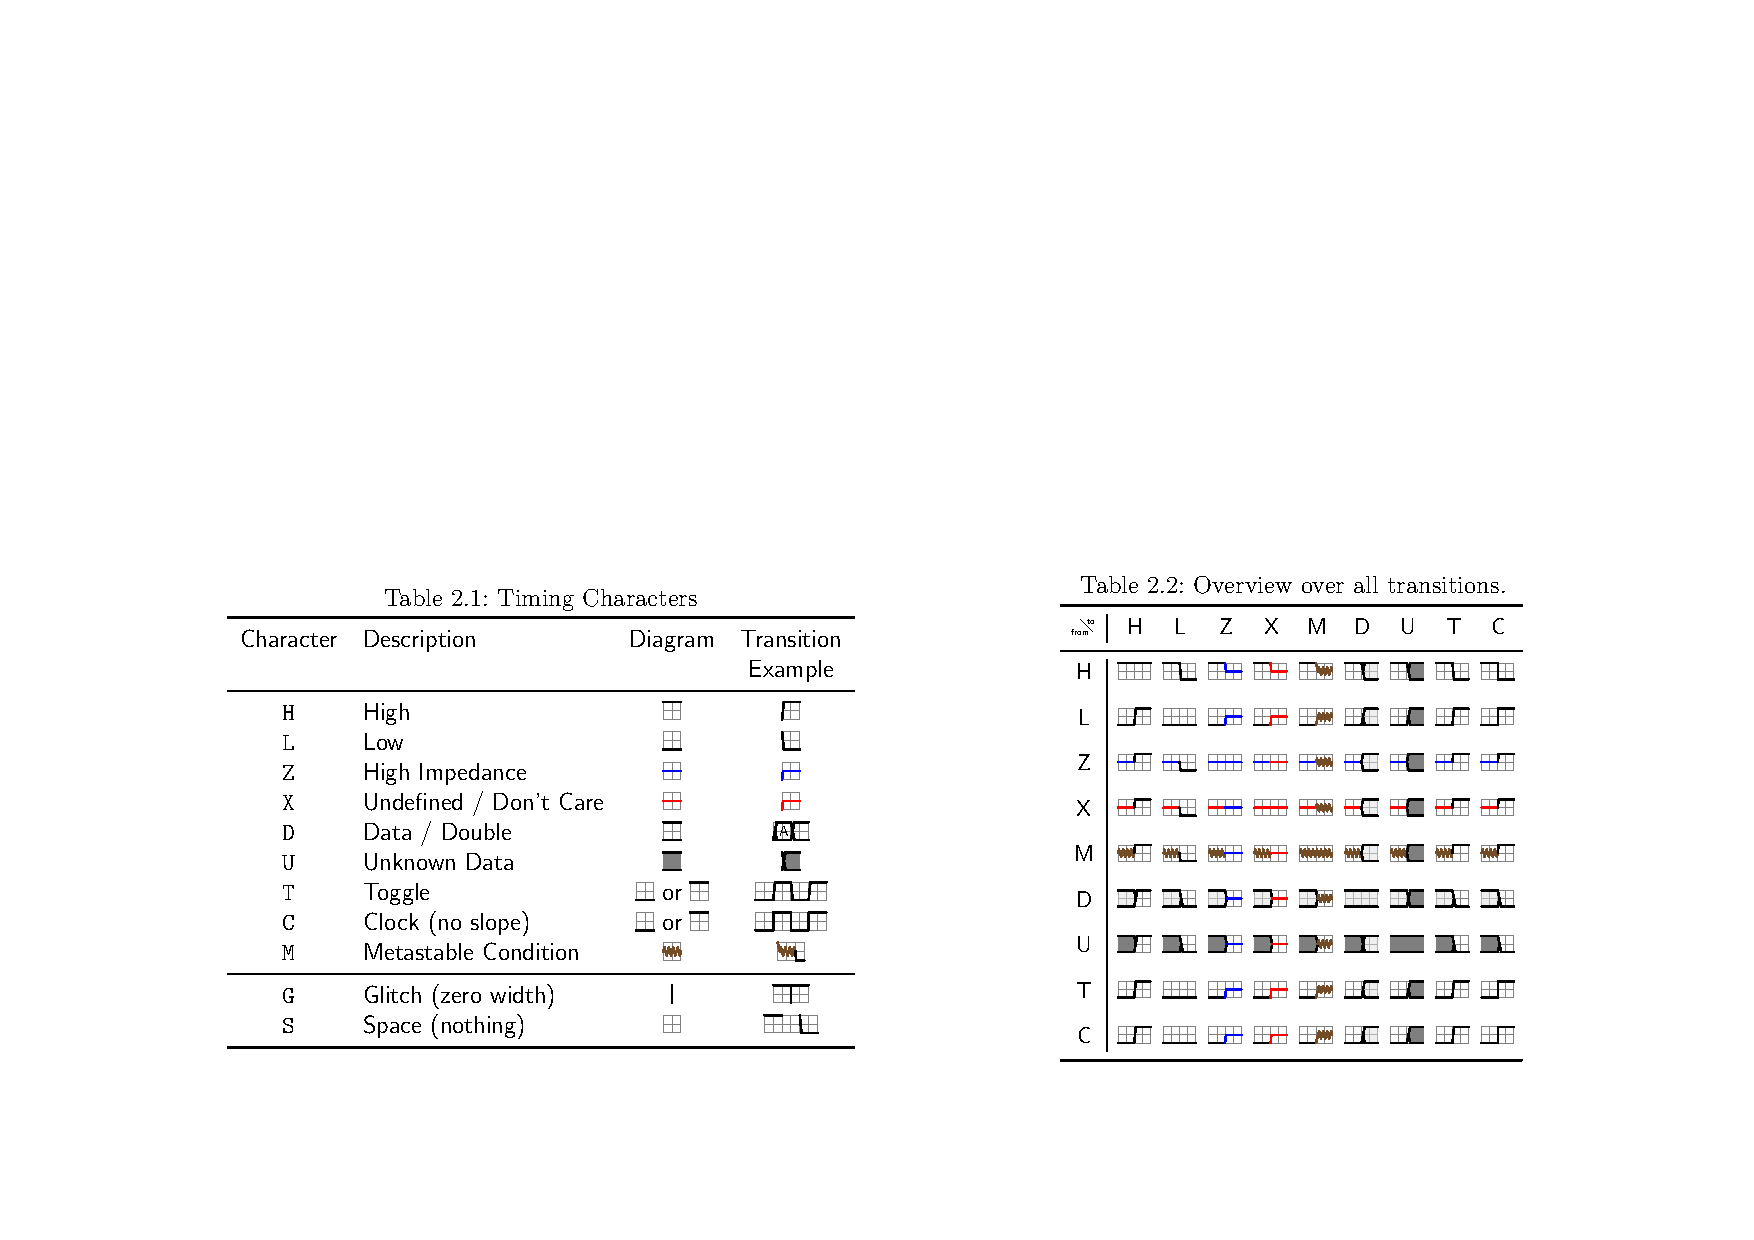
\includegraphics[width=14cm]{tikz-timing/tikz-timing-var_char}\\
  \caption{tikz-timing-char 示意图}\label{tikz-timing-var_char}
\end{figure}

\begin{figure}[H]
  \centering
  % Requires \usepackage{graphicx}
  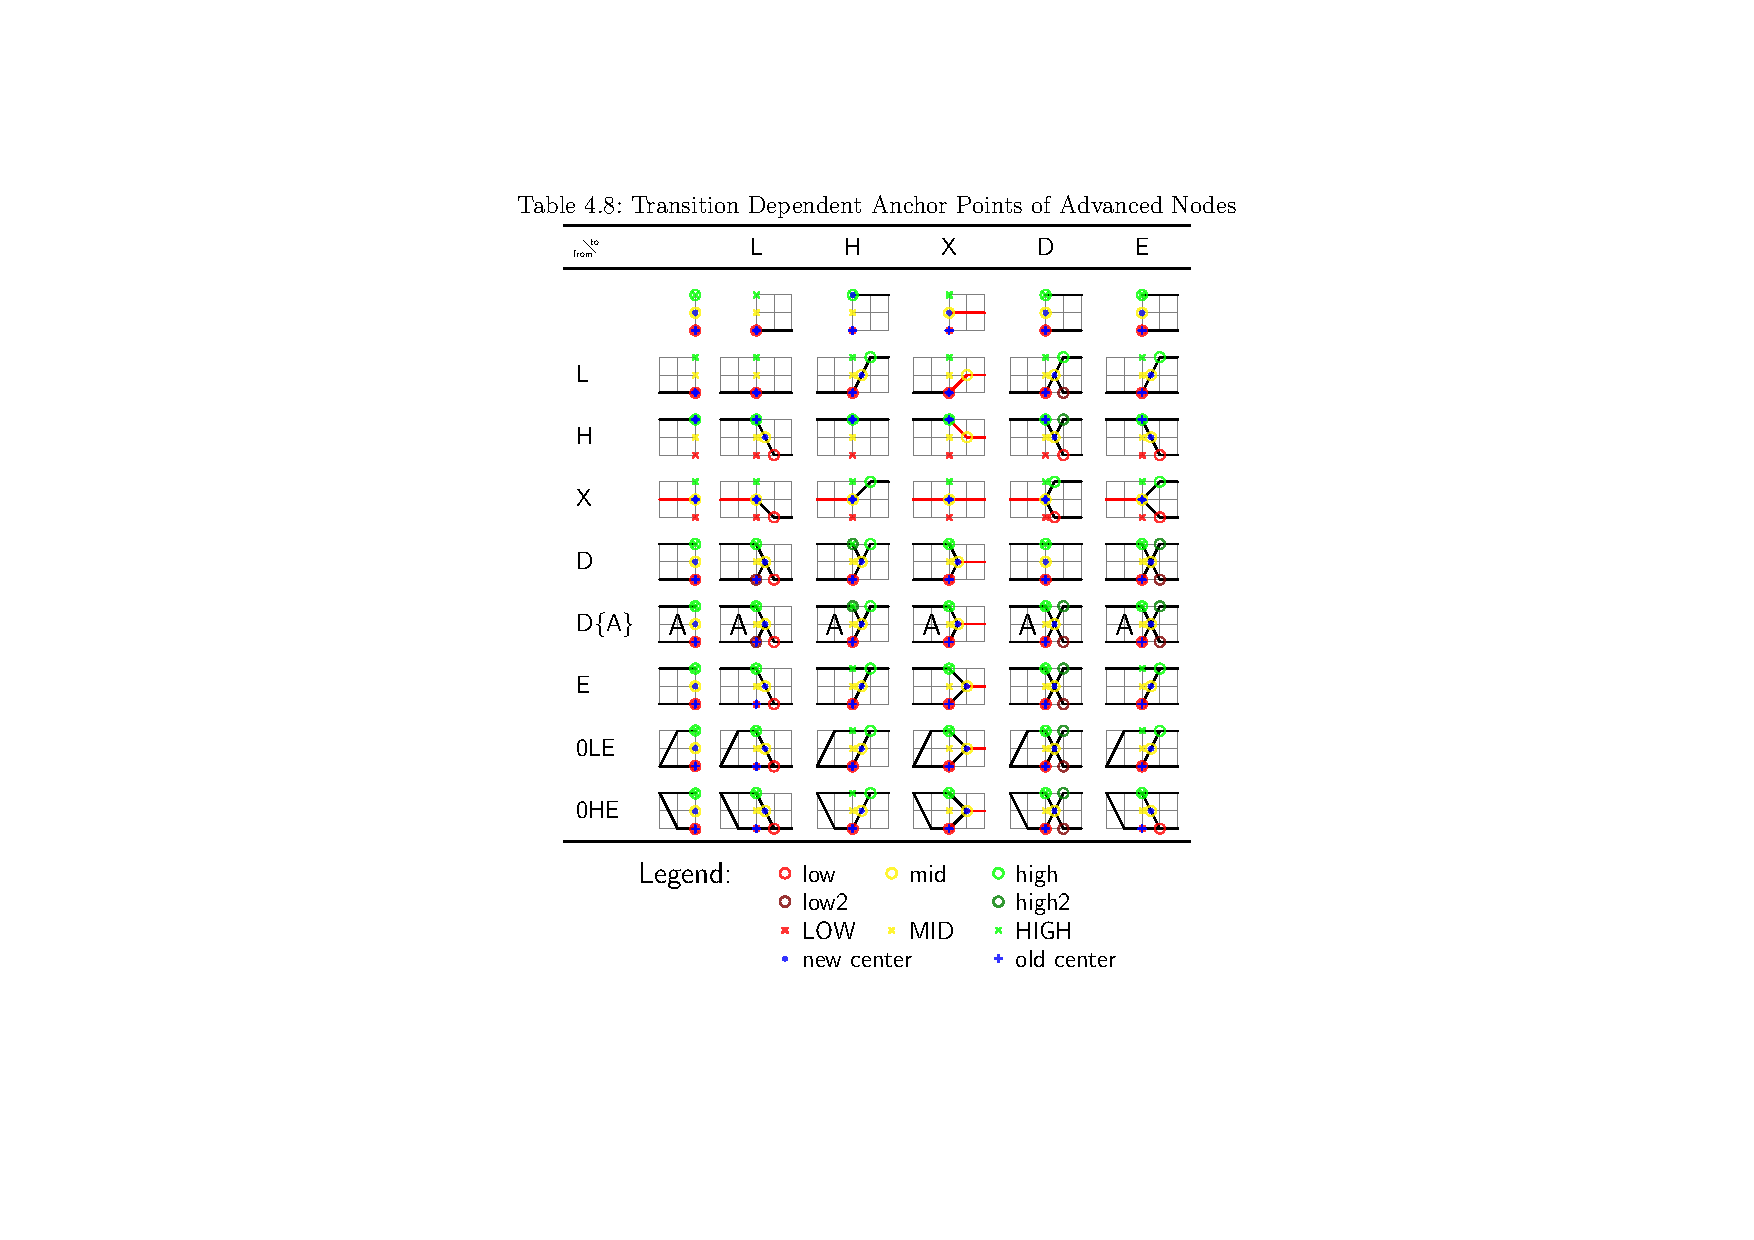
\includegraphics[width=14cm]{tikz-timing/tikz-timing-var_advnodes}\\
  \caption{tikz-timing-advnodes 示意图}\label{tikz-timing-var_advnodes}
\end{figure}

\begin{figure}[H]
  \centering
  % Requires \usepackage{graphicx}
  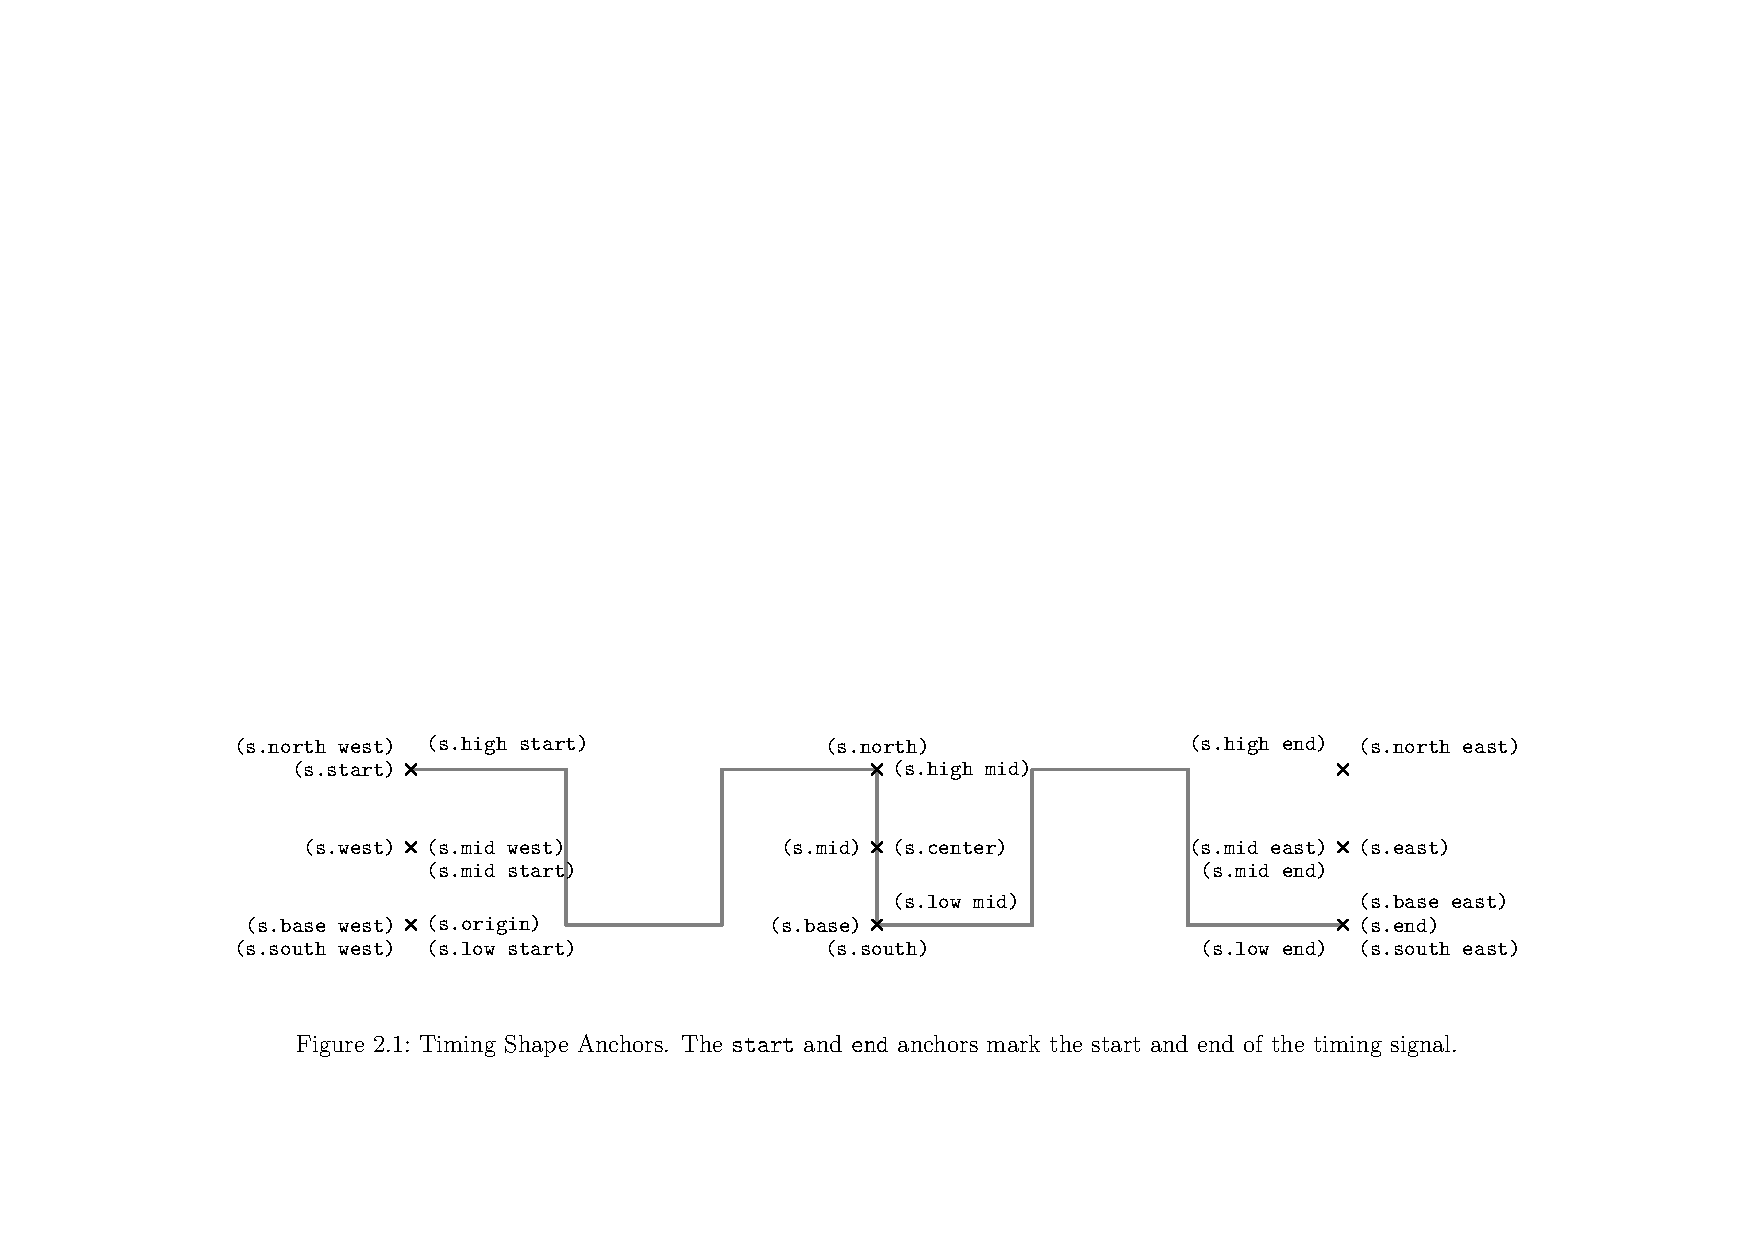
\includegraphics[width=14cm]{tikz-timing/tikz-timing-var_anchor}\\
  \caption{tikz-timing-anchor 示意图}\label{tikz-timing-var_anchor}
\end{figure}


\begin{figure}[H]
  \centering
  % Requires \usepackage{graphicx}
  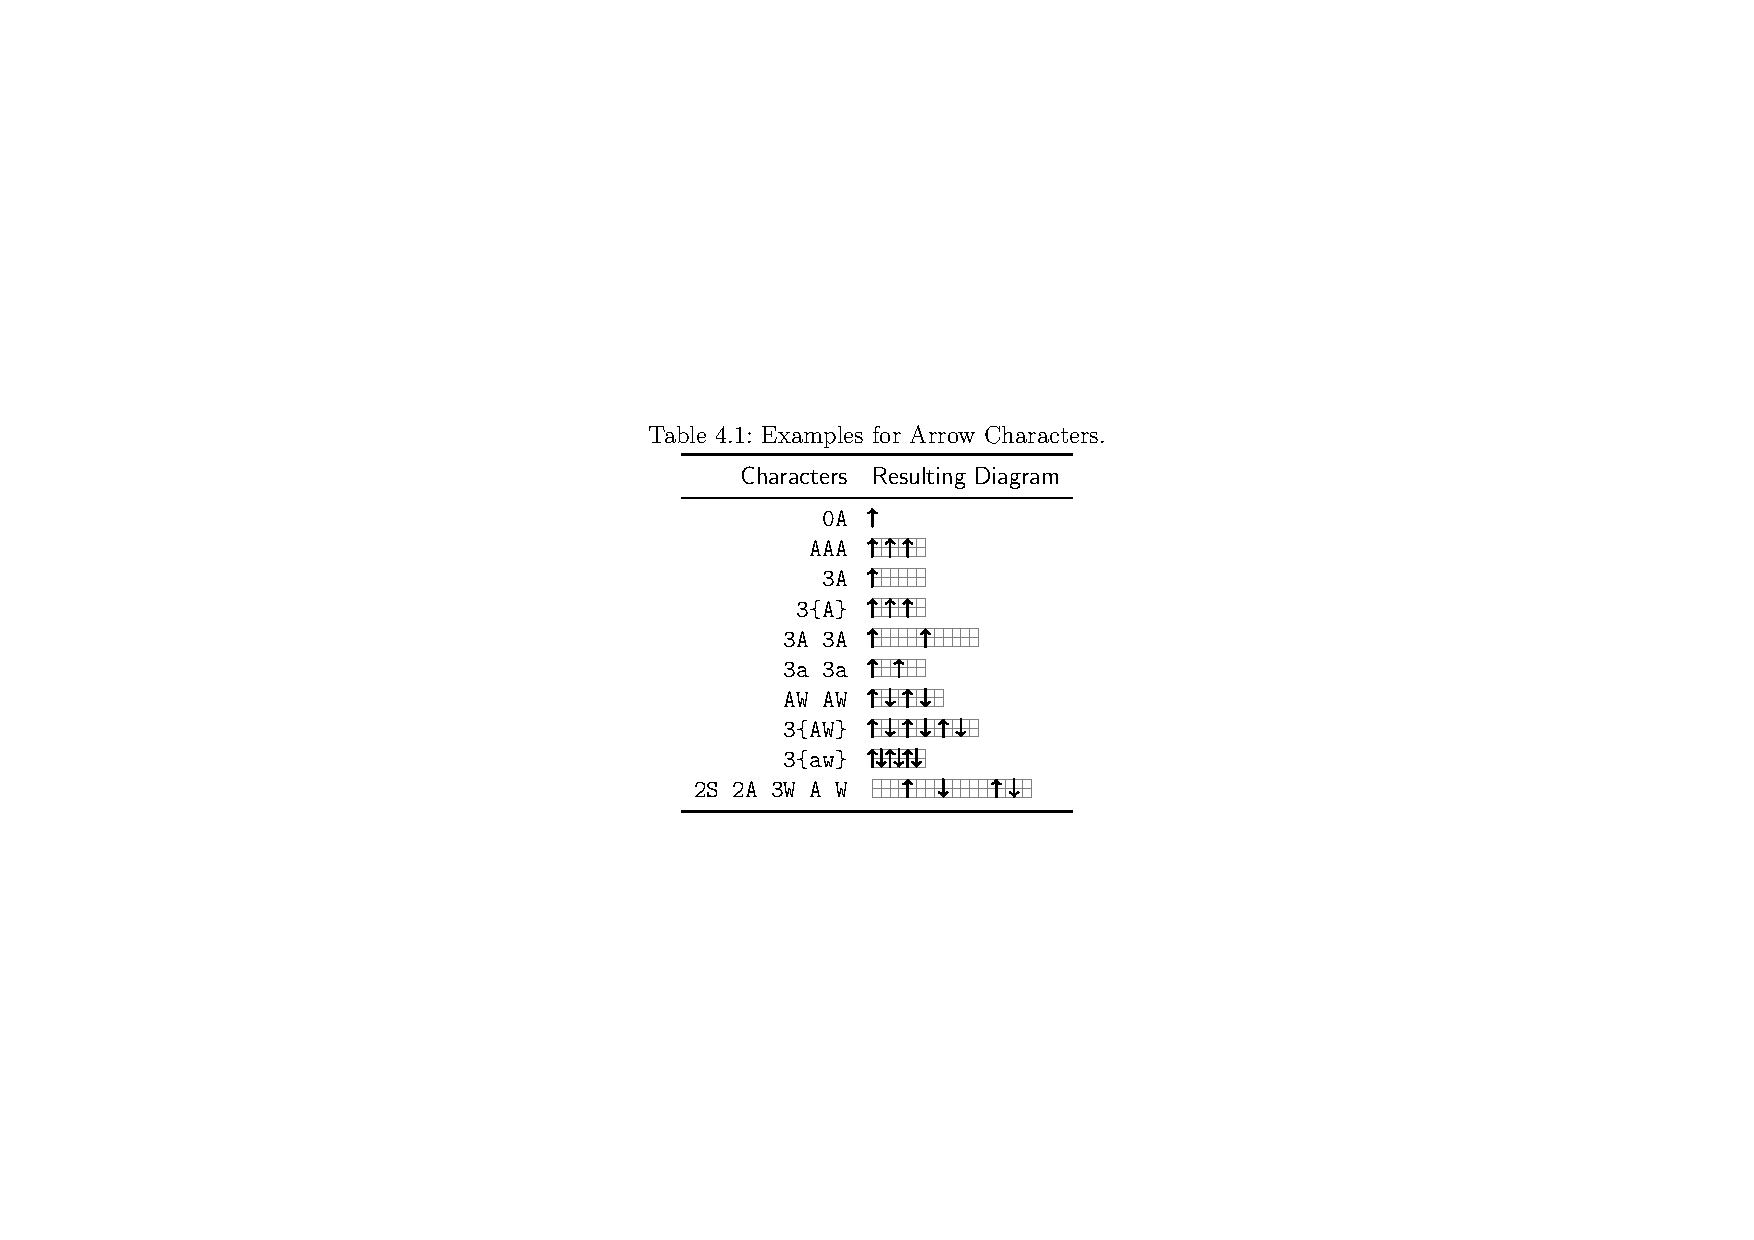
\includegraphics[width=14cm]{tikz-timing/tikz-timing-var_arrow}\\
  \caption{tikz-timing-arrow 示意图}\label{tikz-timing-var_arrow}
\end{figure}


\begin{figure}[H]
  \centering
  % Requires \usepackage{graphicx}
  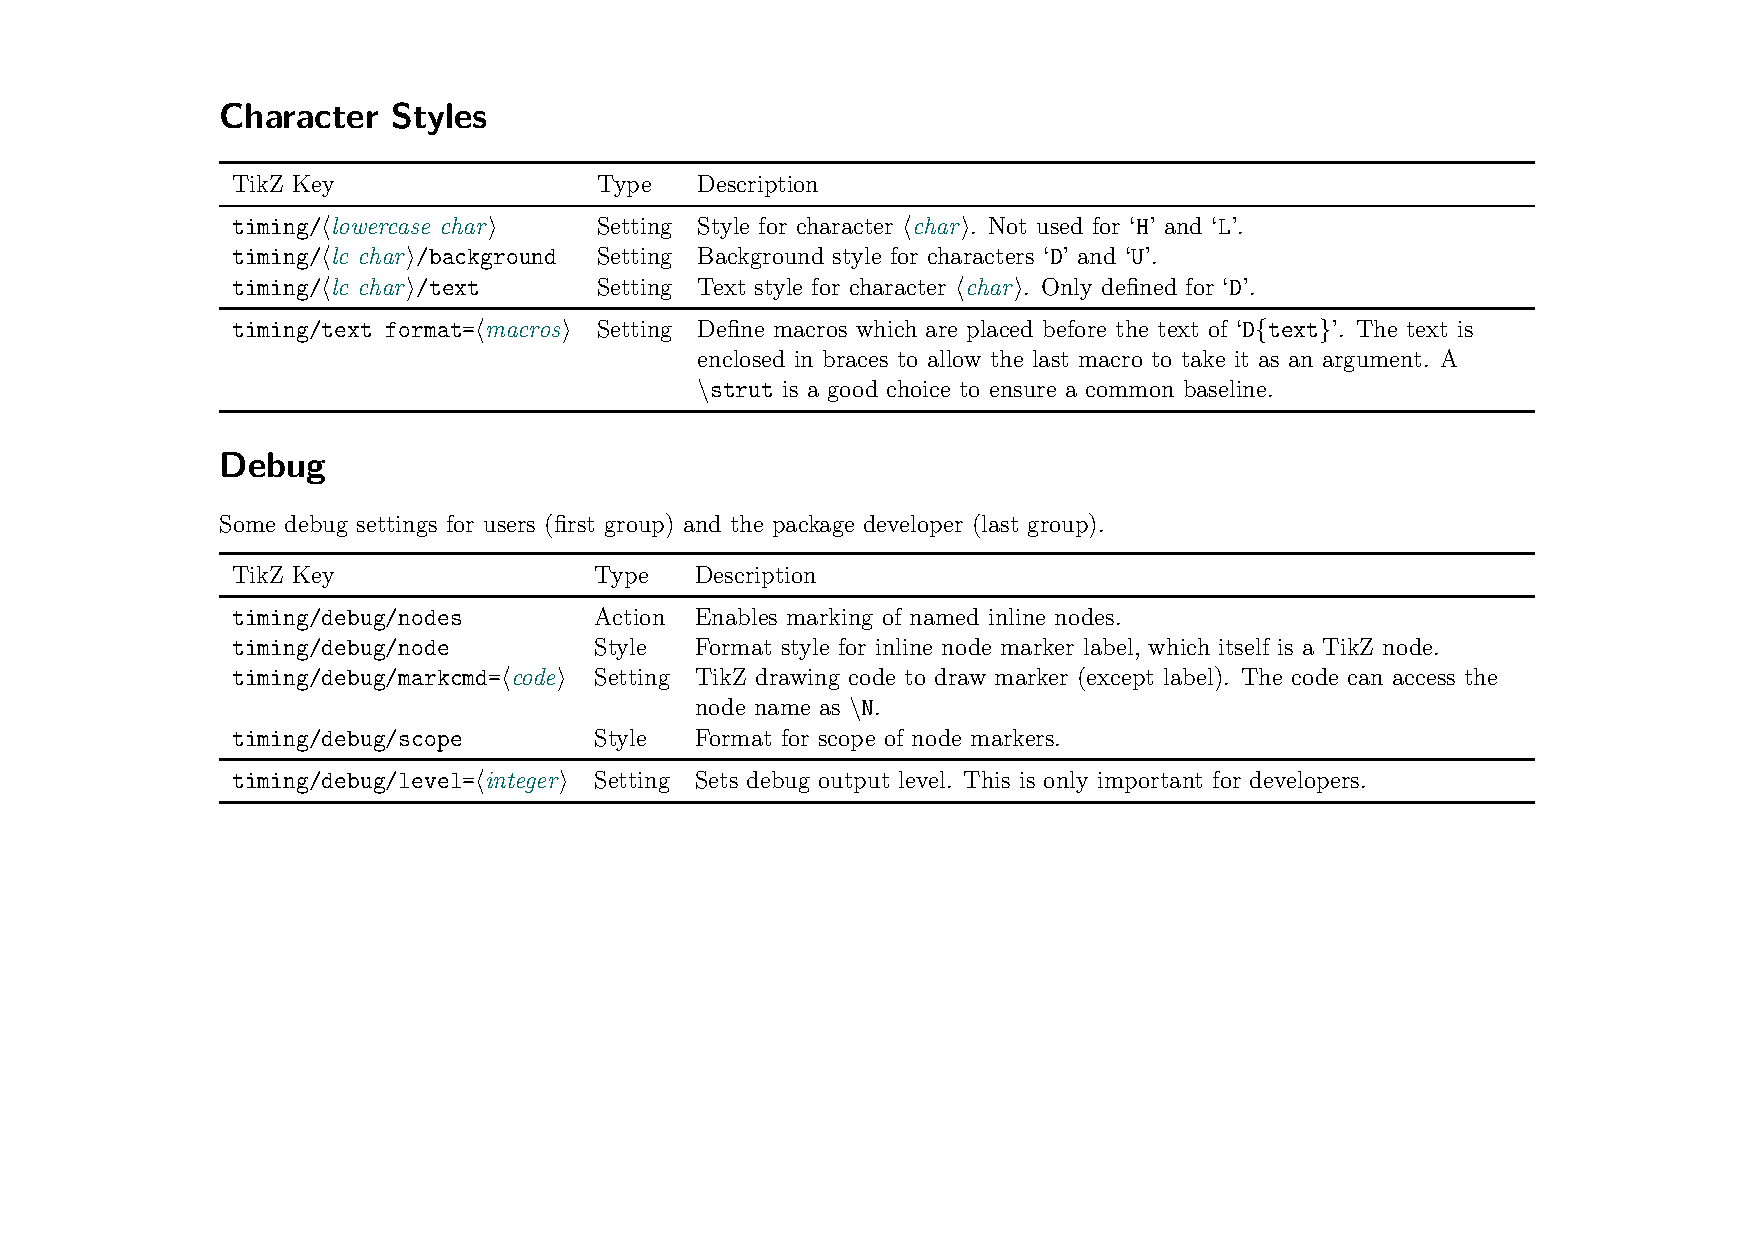
\includegraphics[width=14cm]{tikz-timing/tikz-timing-var_char_debug}\\
  \caption{tikz-timing-char-debug 示意图}\label{tikz-timing-var_char_debug}
\end{figure}


\begin{figure}[H]
  \centering
  % Requires \usepackage{graphicx}
  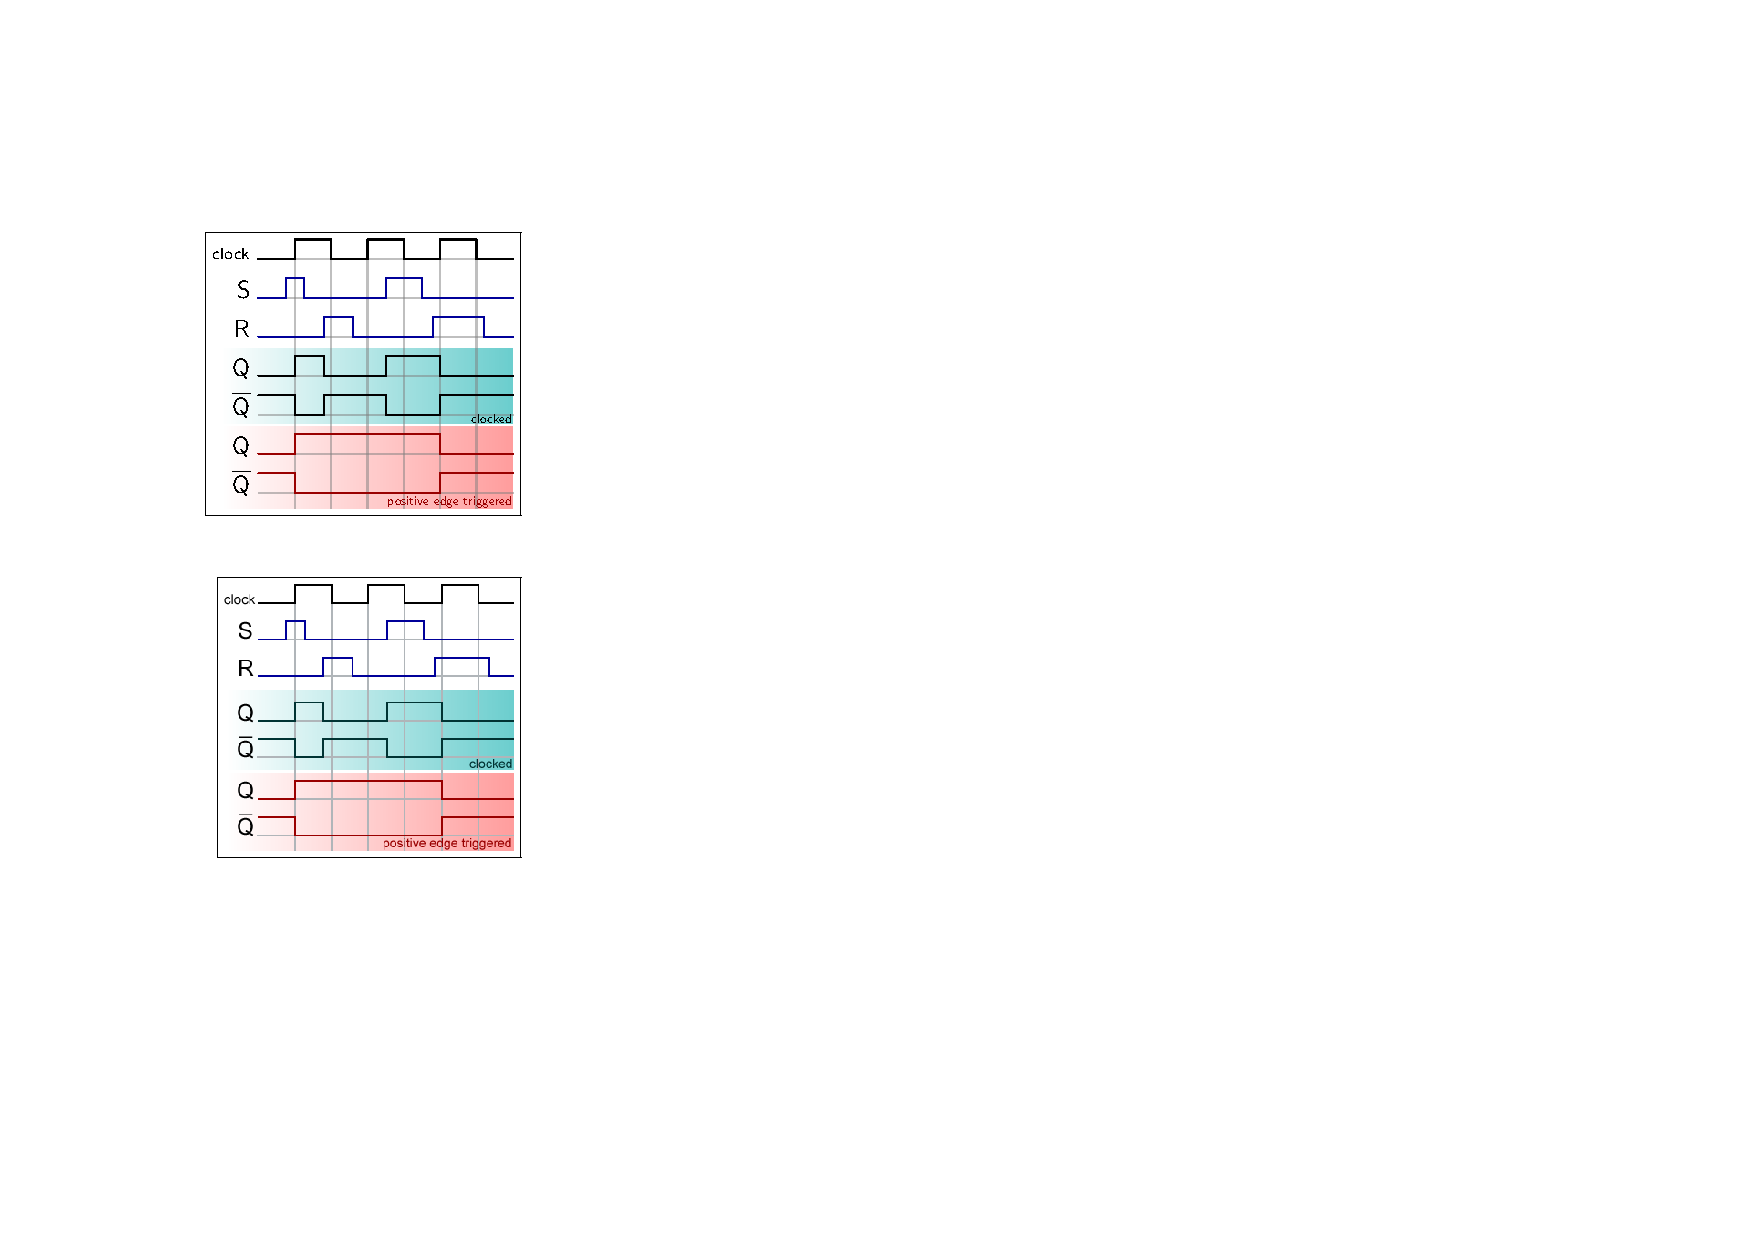
\includegraphics[width=4cm]{tikz-timing/tikz-timing-var_dflip}\\
  \caption{tikz-timing-dflip 示意图}\label{tikz-timing-var_dflip}
\end{figure}


\begin{figure}[]
  \centering
  % Requires \usepackage{graphicx}
  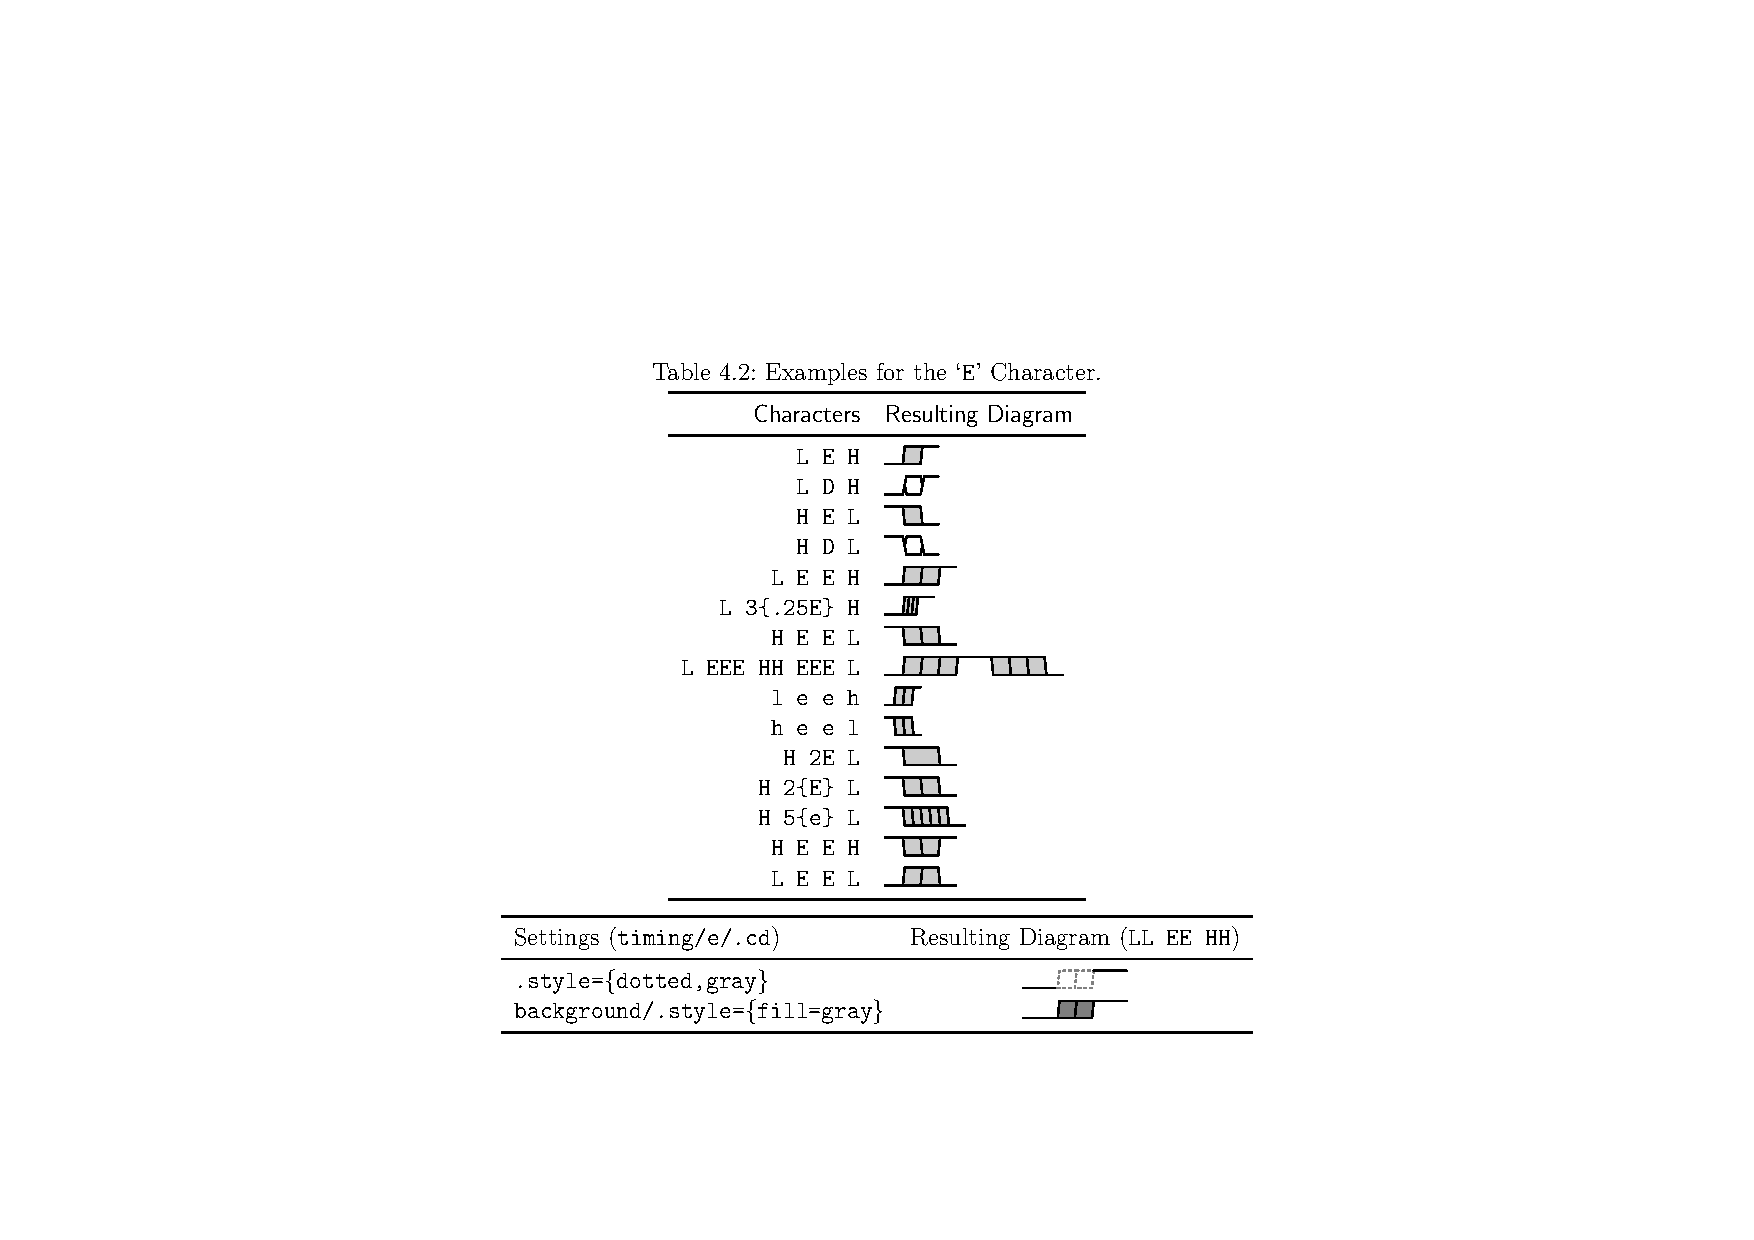
\includegraphics[width=14cm]{tikz-timing/tikz-timing-var_e}\\
  \caption{tikz-timing-e 示意图}\label{tikz-timing-var_anchor}
\end{figure}
\begin{table}[H]
  \centering
  % Requires \usepackage{graphicx}
  \caption{tikz-timing-E E符号对应表}\label{tikz-timing-var_ex3}
  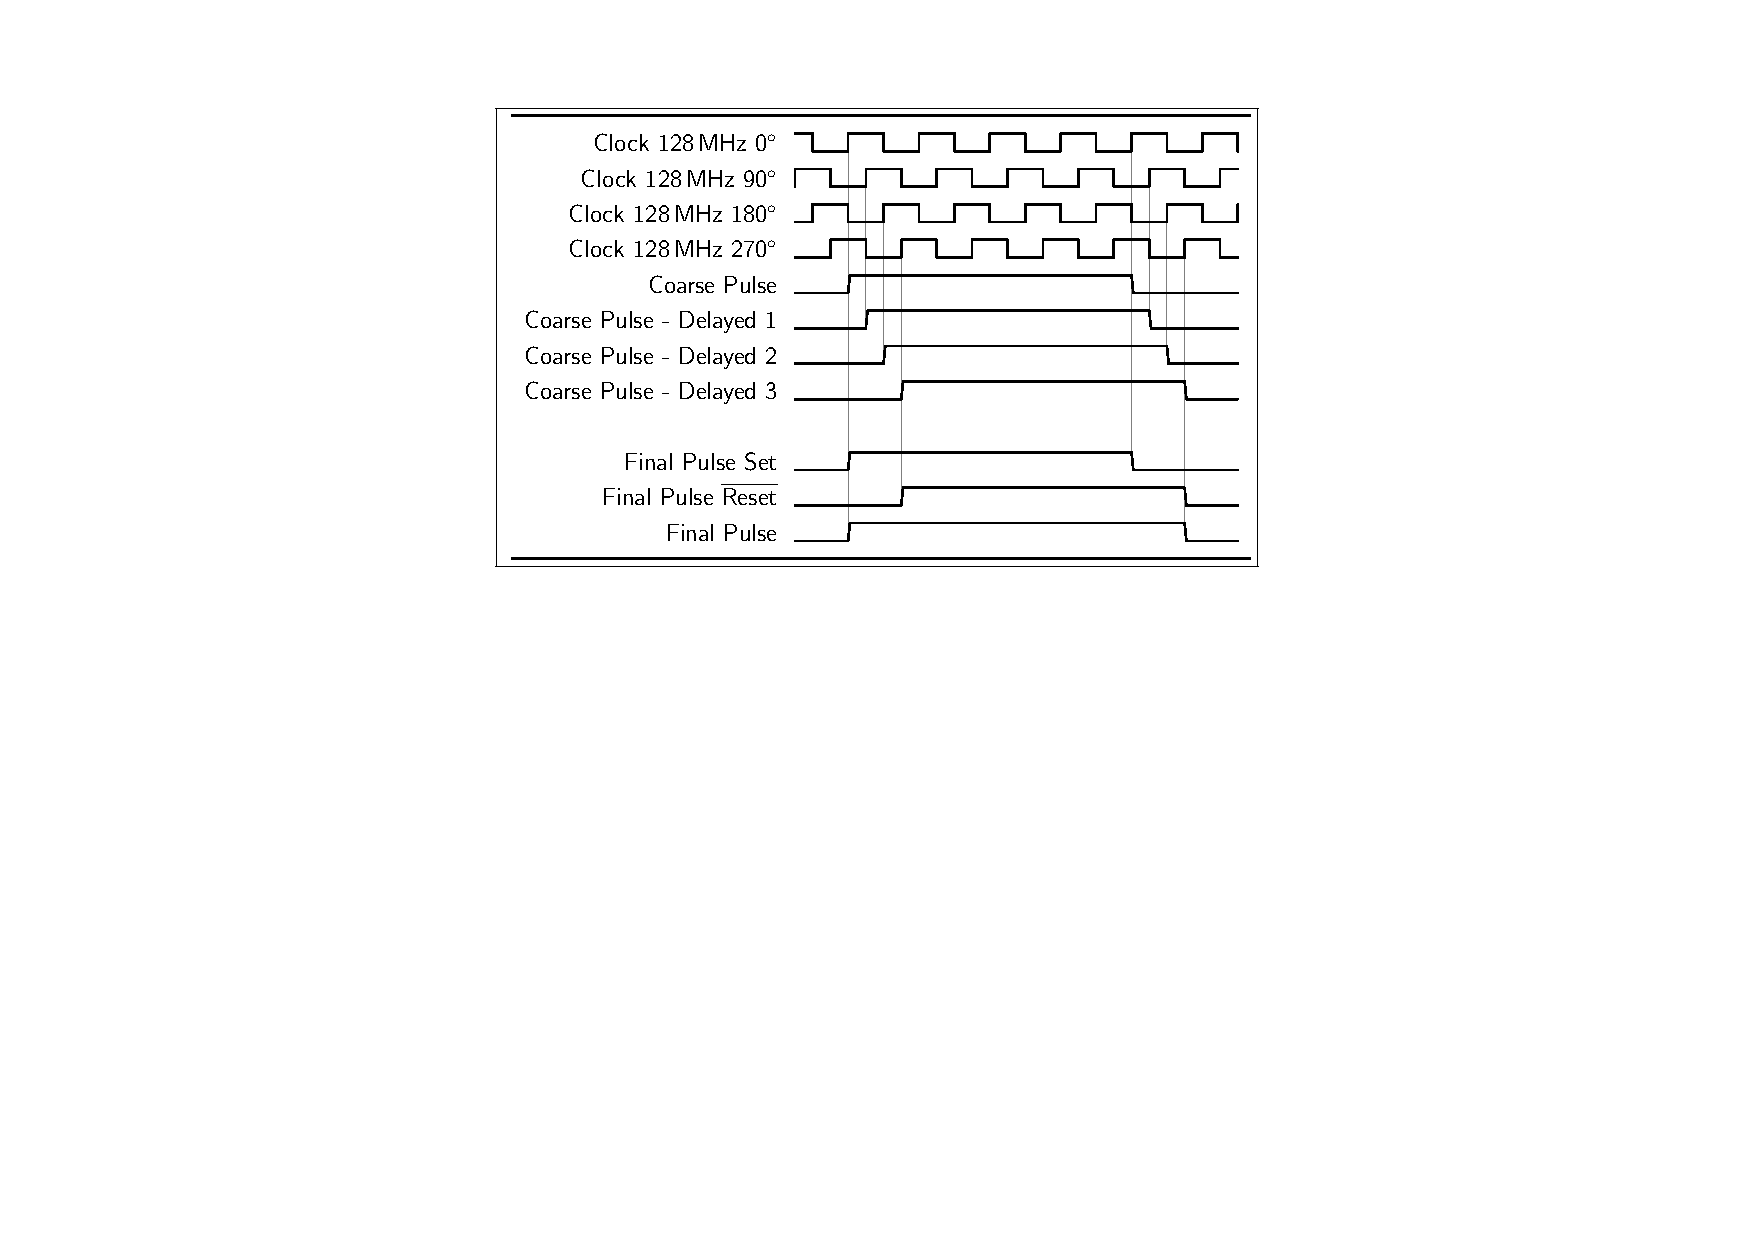
\includegraphics[width=14cm]{tikz-timing/tikz-timing-var_ex3}\\
\end{table}
\begin{figure}[H]
  \centering
  % Requires \usepackage{graphicx}
  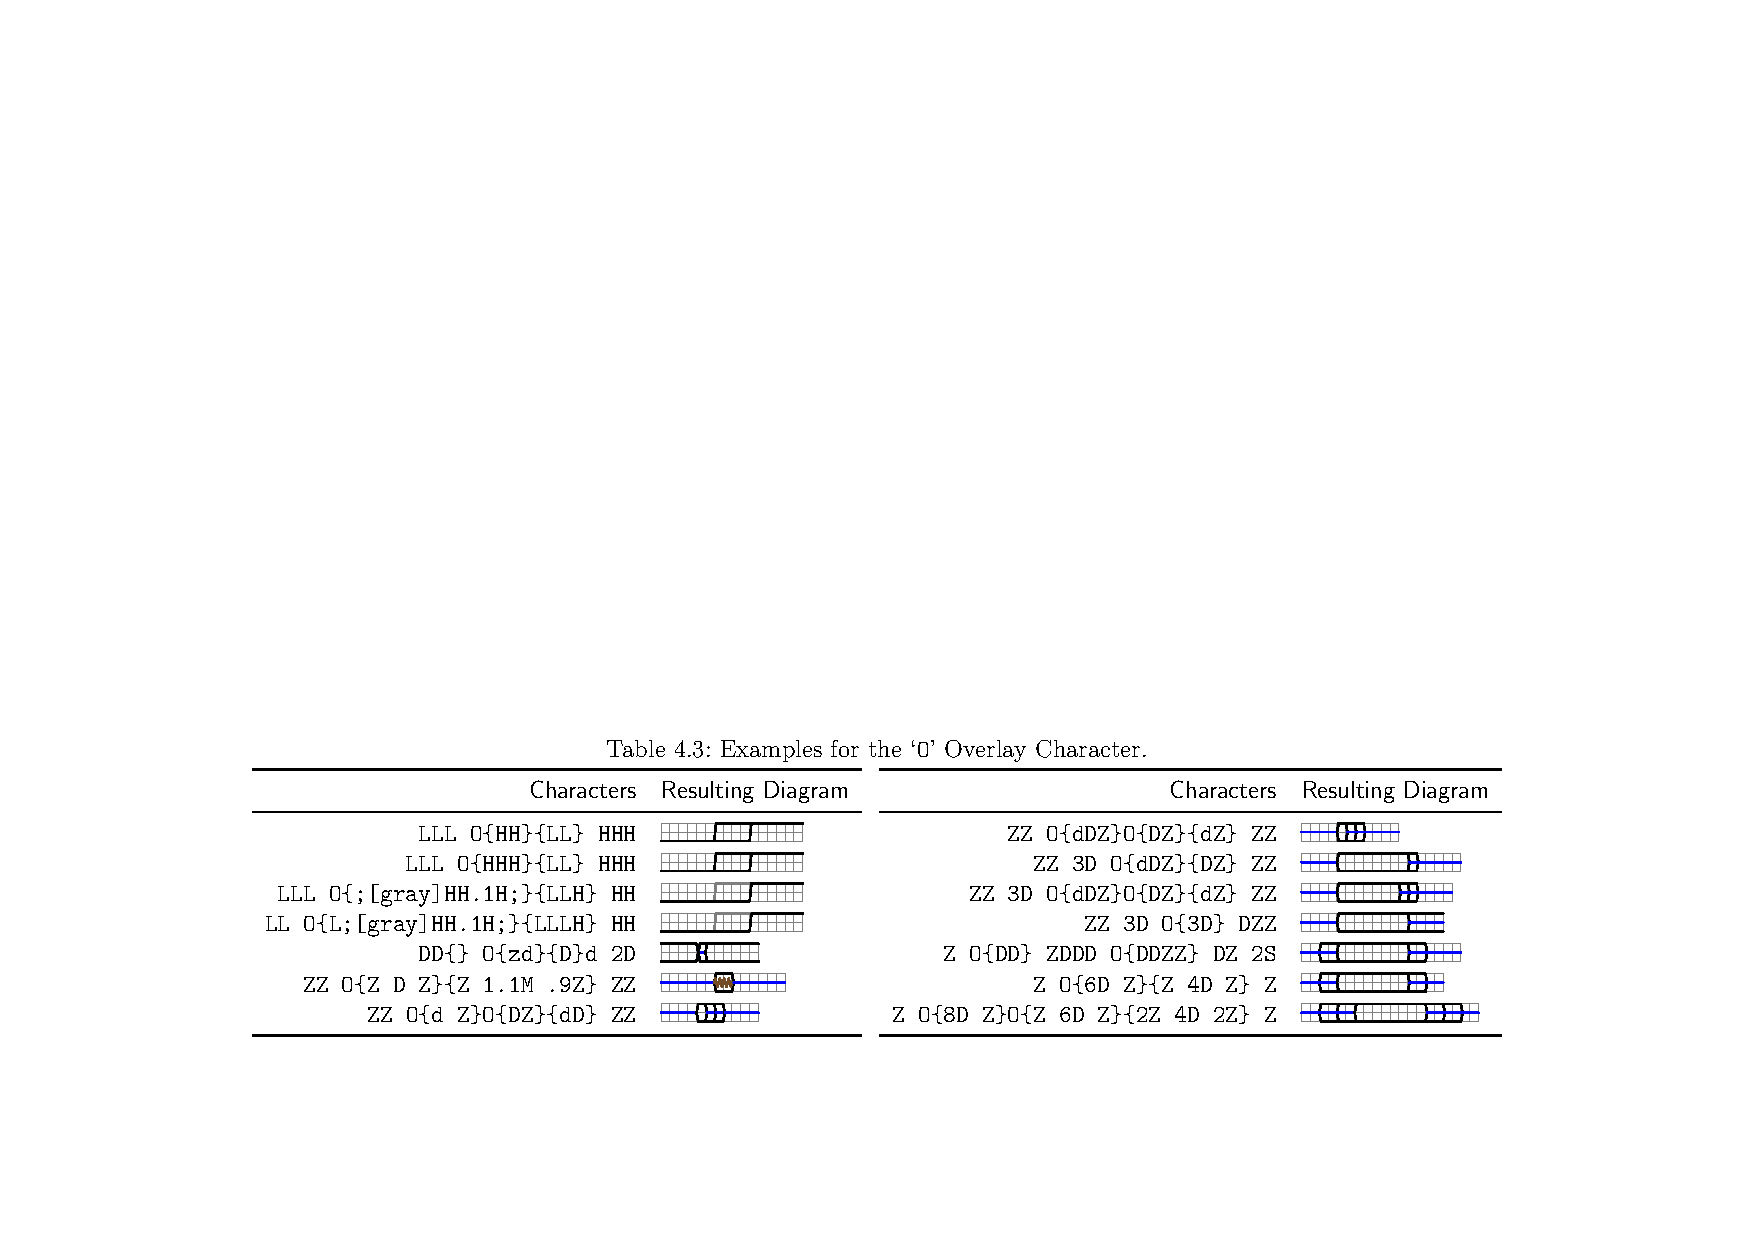
\includegraphics[width=14cm]{tikz-timing/tikz-timing-var_o}\\
  \caption{tikz-timing-o 示意图}\label{tikz-timing-var_o}
\end{figure}

\begin{figure}[H]
  \centering
  % Requires \usepackage{graphicx}
  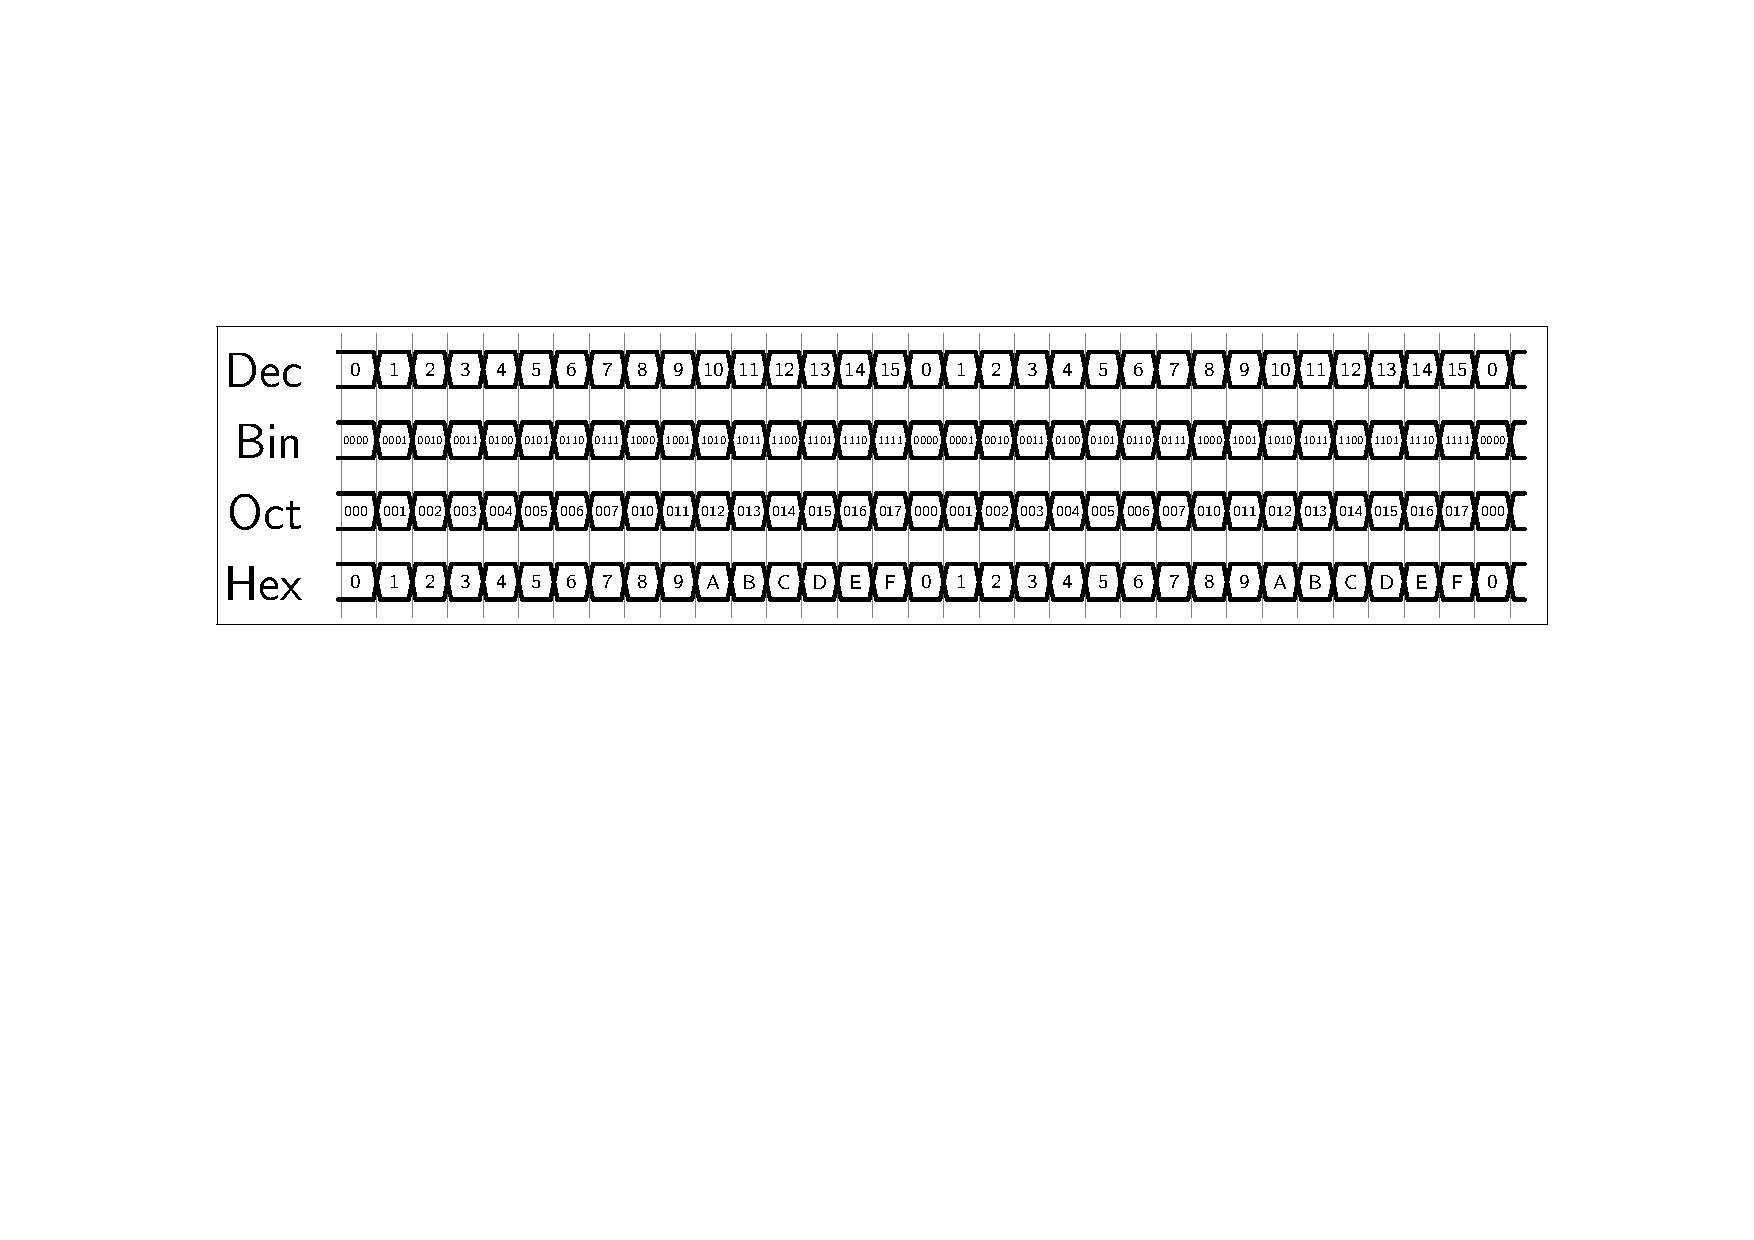
\includegraphics[width=14cm]{tikz-timing/tikz-timing-var_ex1}\\
  \caption{tikz-timing-ex1 示意图}\label{tikz-timing-var_ex1}
\end{figure}
\begin{figure}[H]
  \centering
  % Requires \usepackage{graphicx}
  
\includegraphics[width=4cm]{tikz-timing/tikz-timing-var_ex2}\\
  \caption{tikz-timing-ex2 示意图}\label{tikz-timing-var_ex2}
\end{figure}
\begin{figure}[H]
  \centering
  % Requires \usepackage{graphicx}
  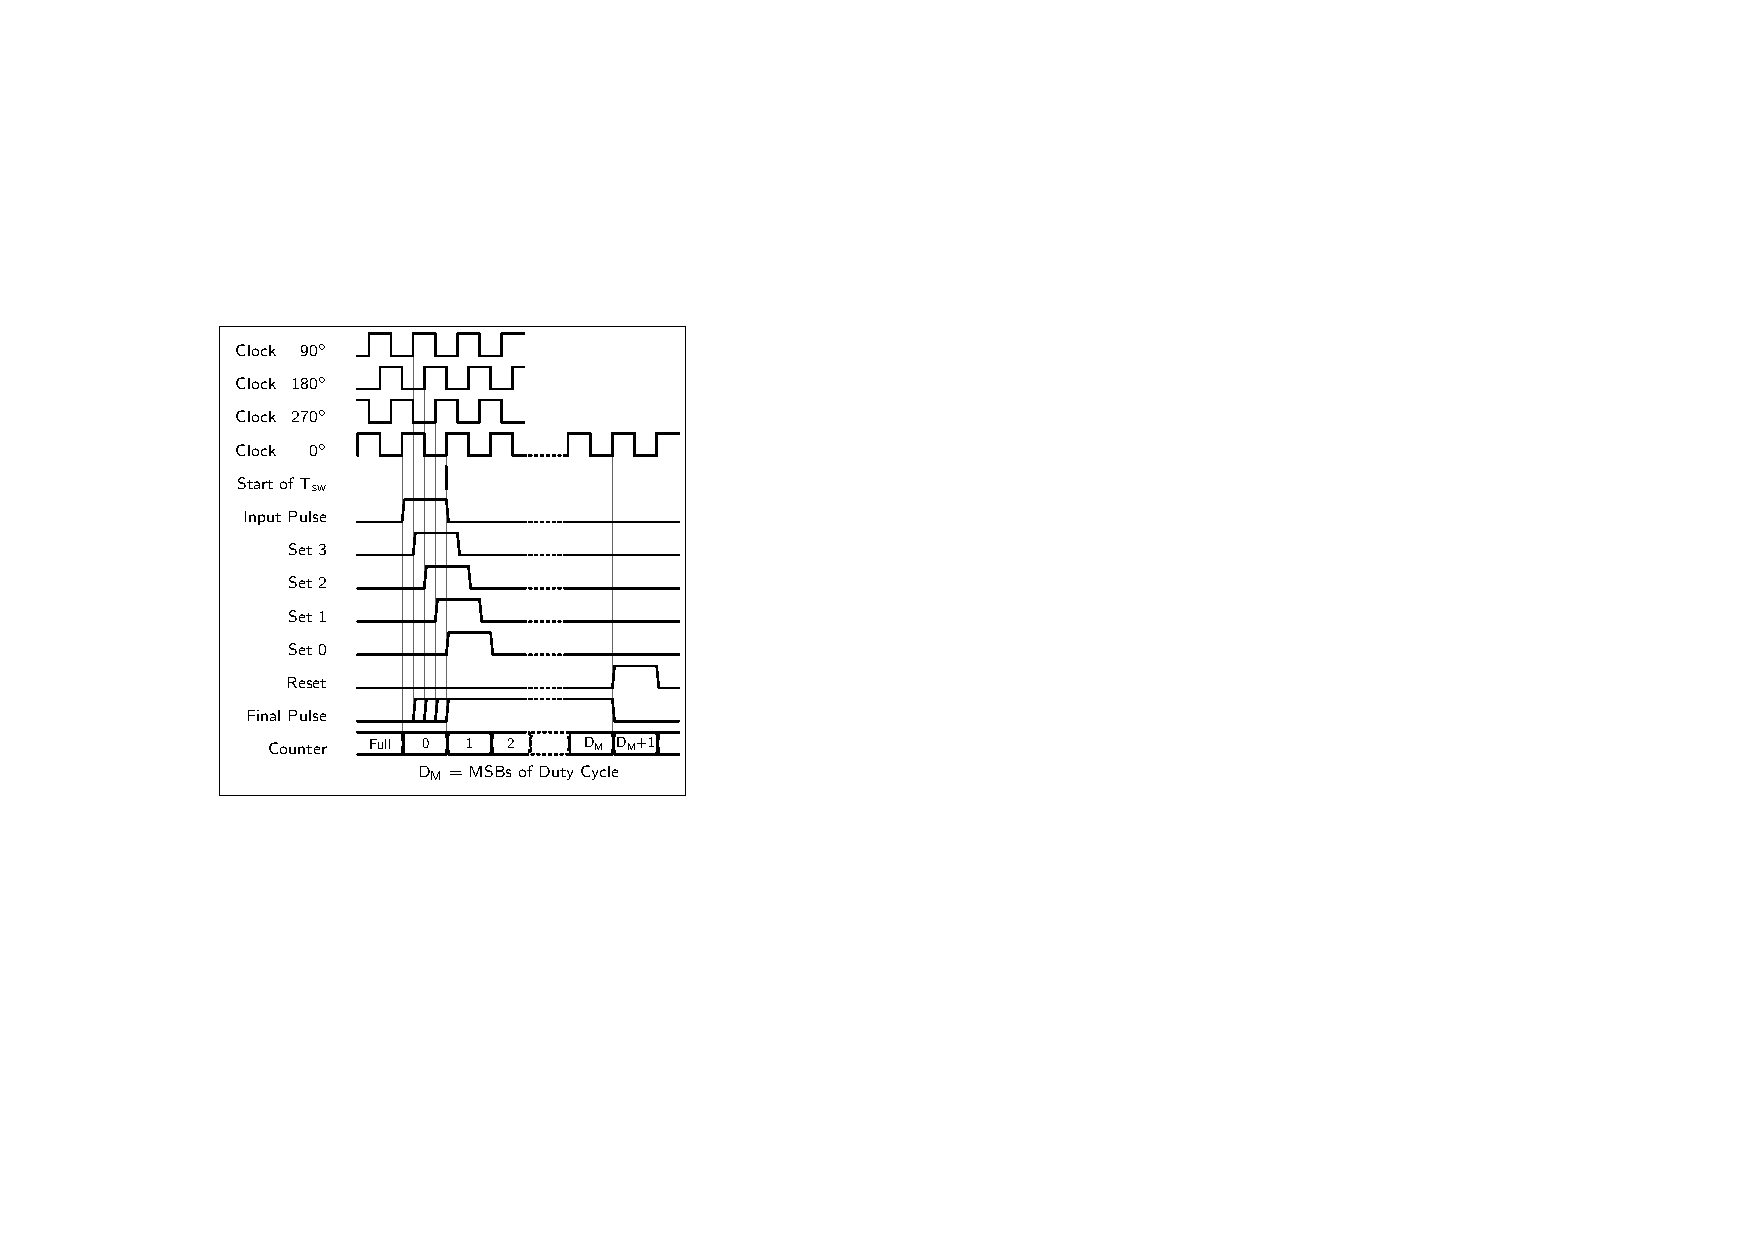
\includegraphics[width=14cm]{tikz-timing/tikz-timing-var_ex4}\\
  \caption{tikz-timing-ex4 示意图}\label{tikz-timing-var_ex4}
\end{figure}

\begin{table}[H]
  \centering
  % Requires \usepackage{graphicx}
    \caption{tikz-timing-grid-table 参数表}\label{tikz-timing-var_grid_table}
  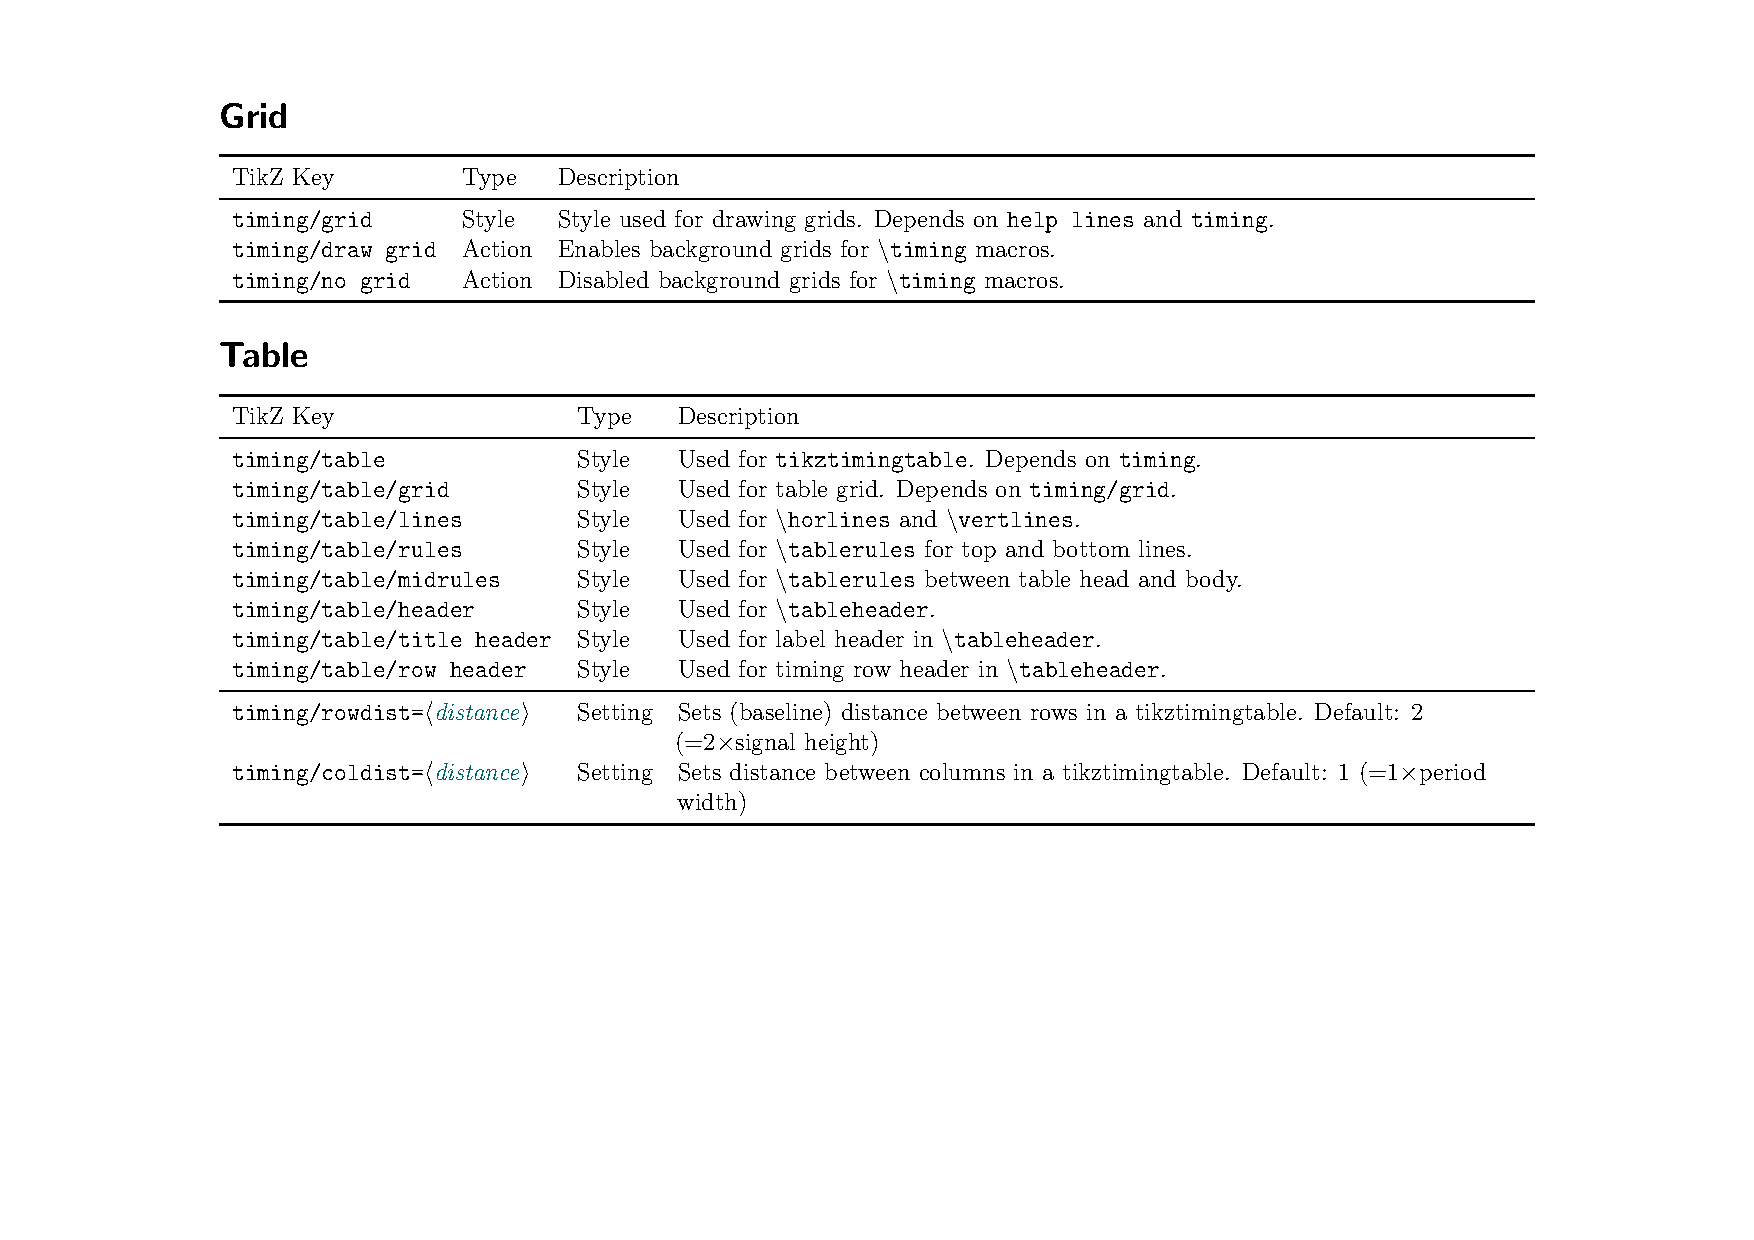
\includegraphics[width=14cm]{tikz-timing/tikz-timing-var_grid_table}\\
\end{table}

\begin{table}[H]
  \centering
  % Requires \usepackage{graphicx}
    \caption{tikz-timing-grid-ifsym 参数表}\label{tikz-timing-var_grid_ifsym}
  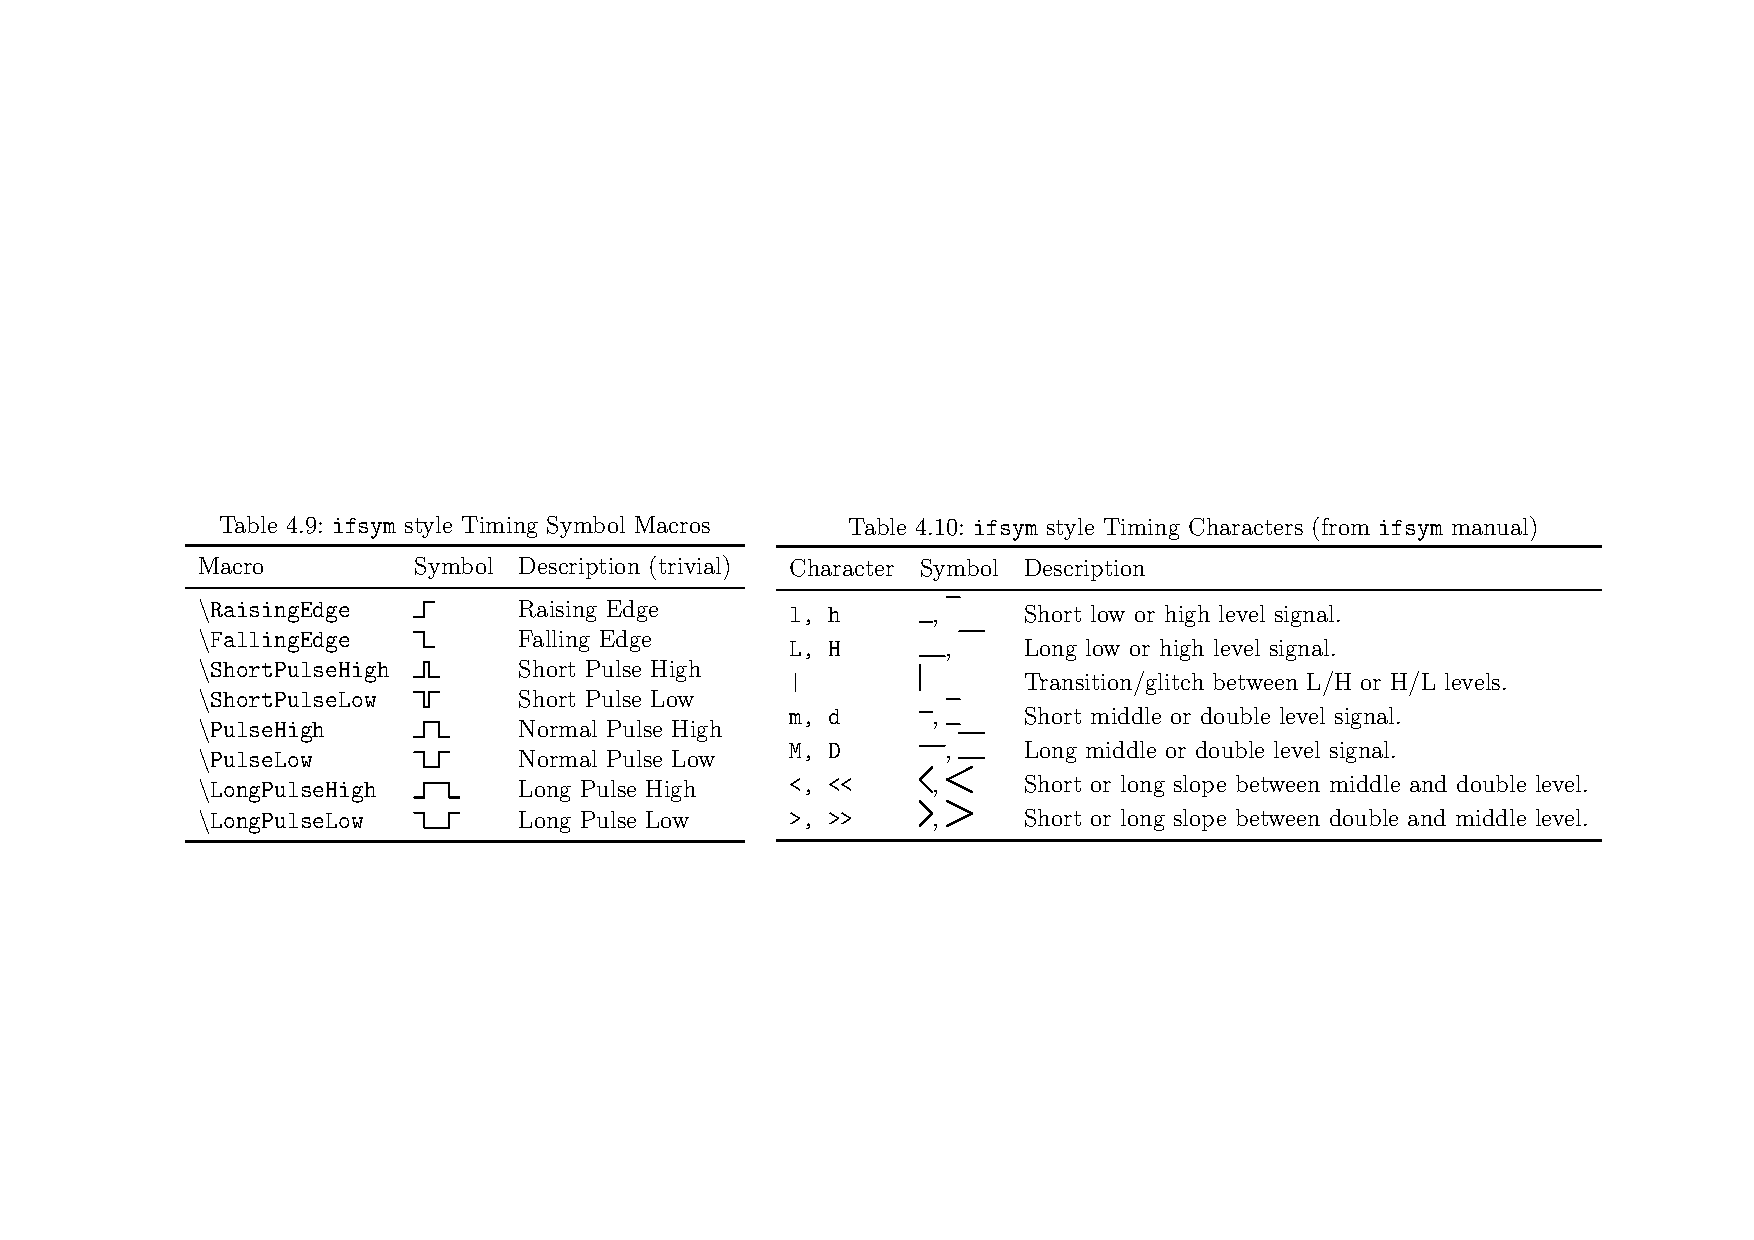
\includegraphics[width=14cm]{tikz-timing/tikz-timing-var_ifsym}\\
\end{table}

\begin{figure}[H]
  \centering
  % Requires \usepackage{graphicx}
  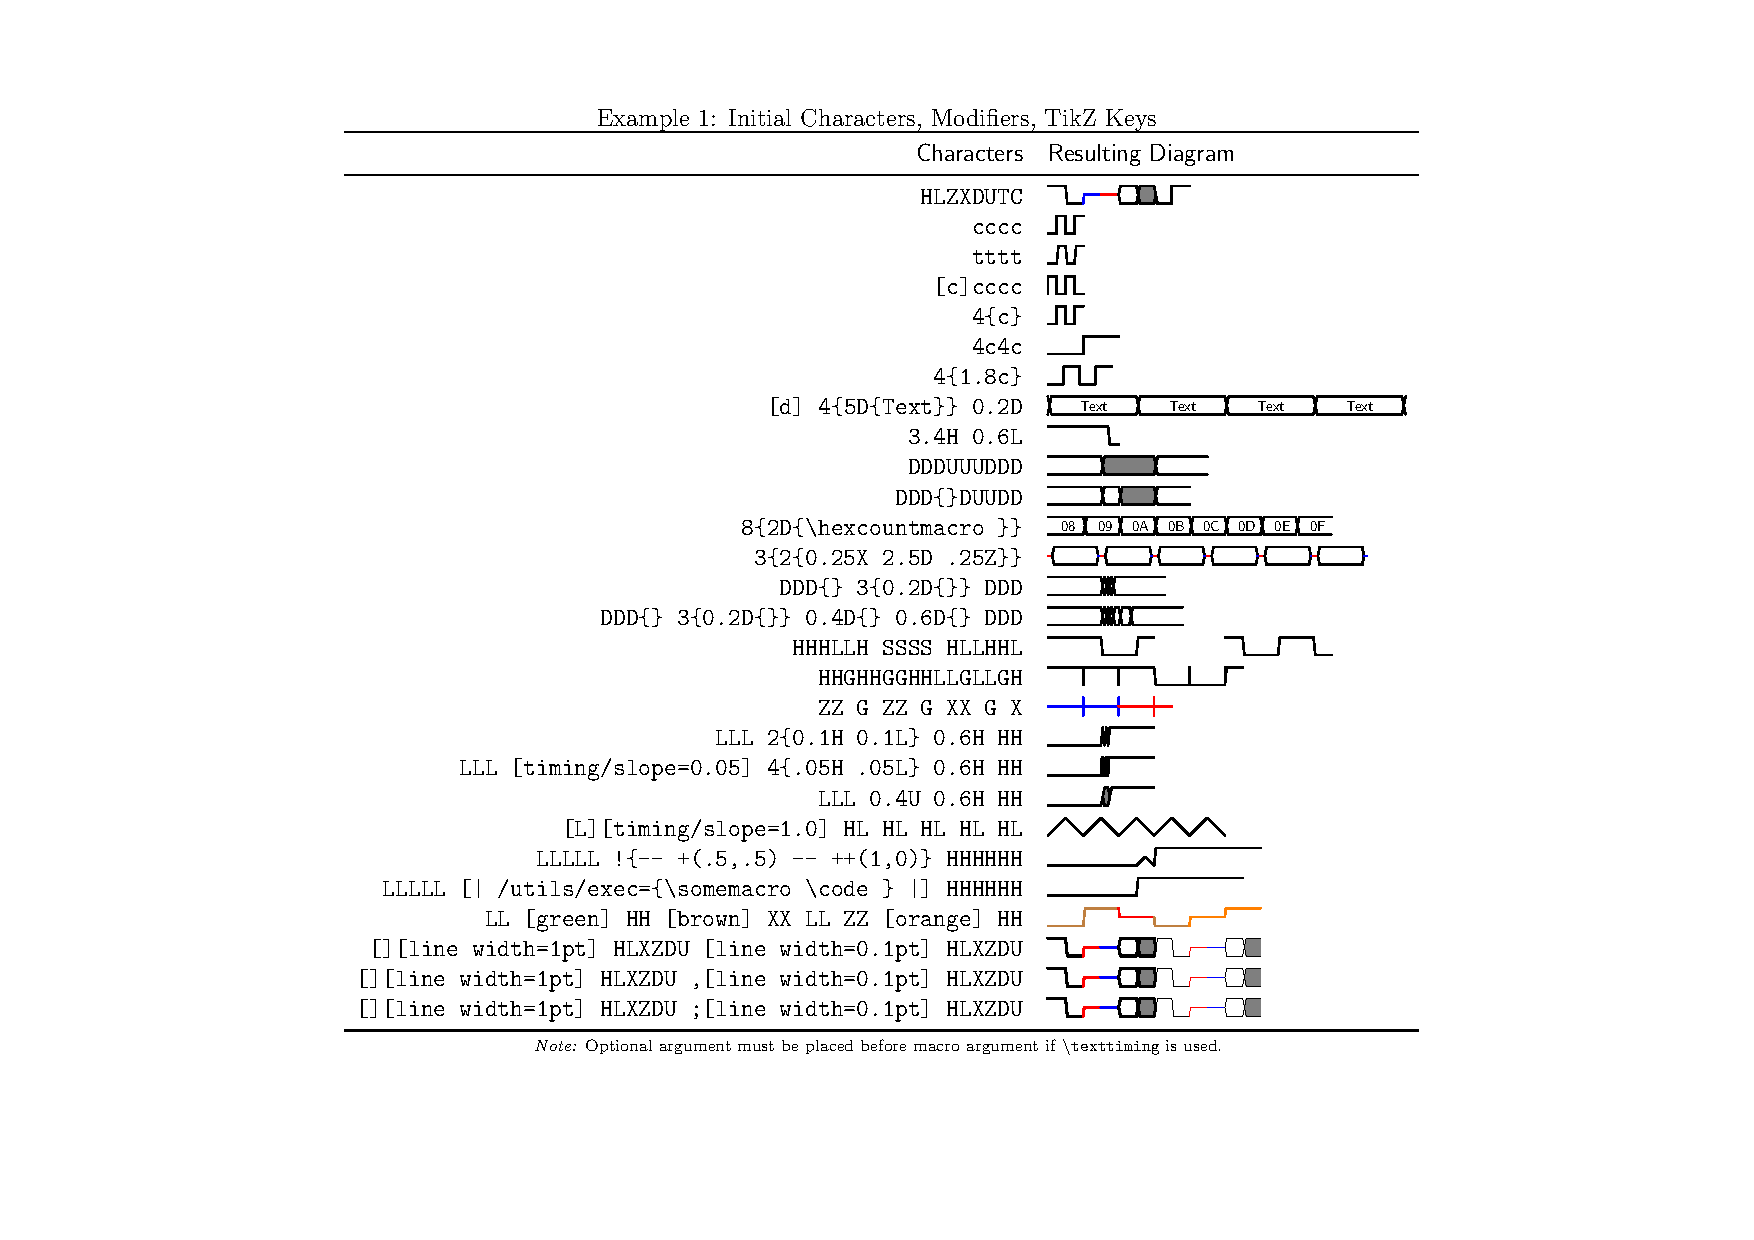
\includegraphics[width=14cm]{tikz-timing/tikz-timing-var_initial}\\
  \caption{tikz-timing-initial 初始化图}\label{tikz-timing-var_initial}
\end{figure}

\begin{table}[H]
  \centering
  % Requires \usepackage{graphicx}
    \caption{tikz-timing-meta 参数表}\label{tikz-timing-var_meta}
  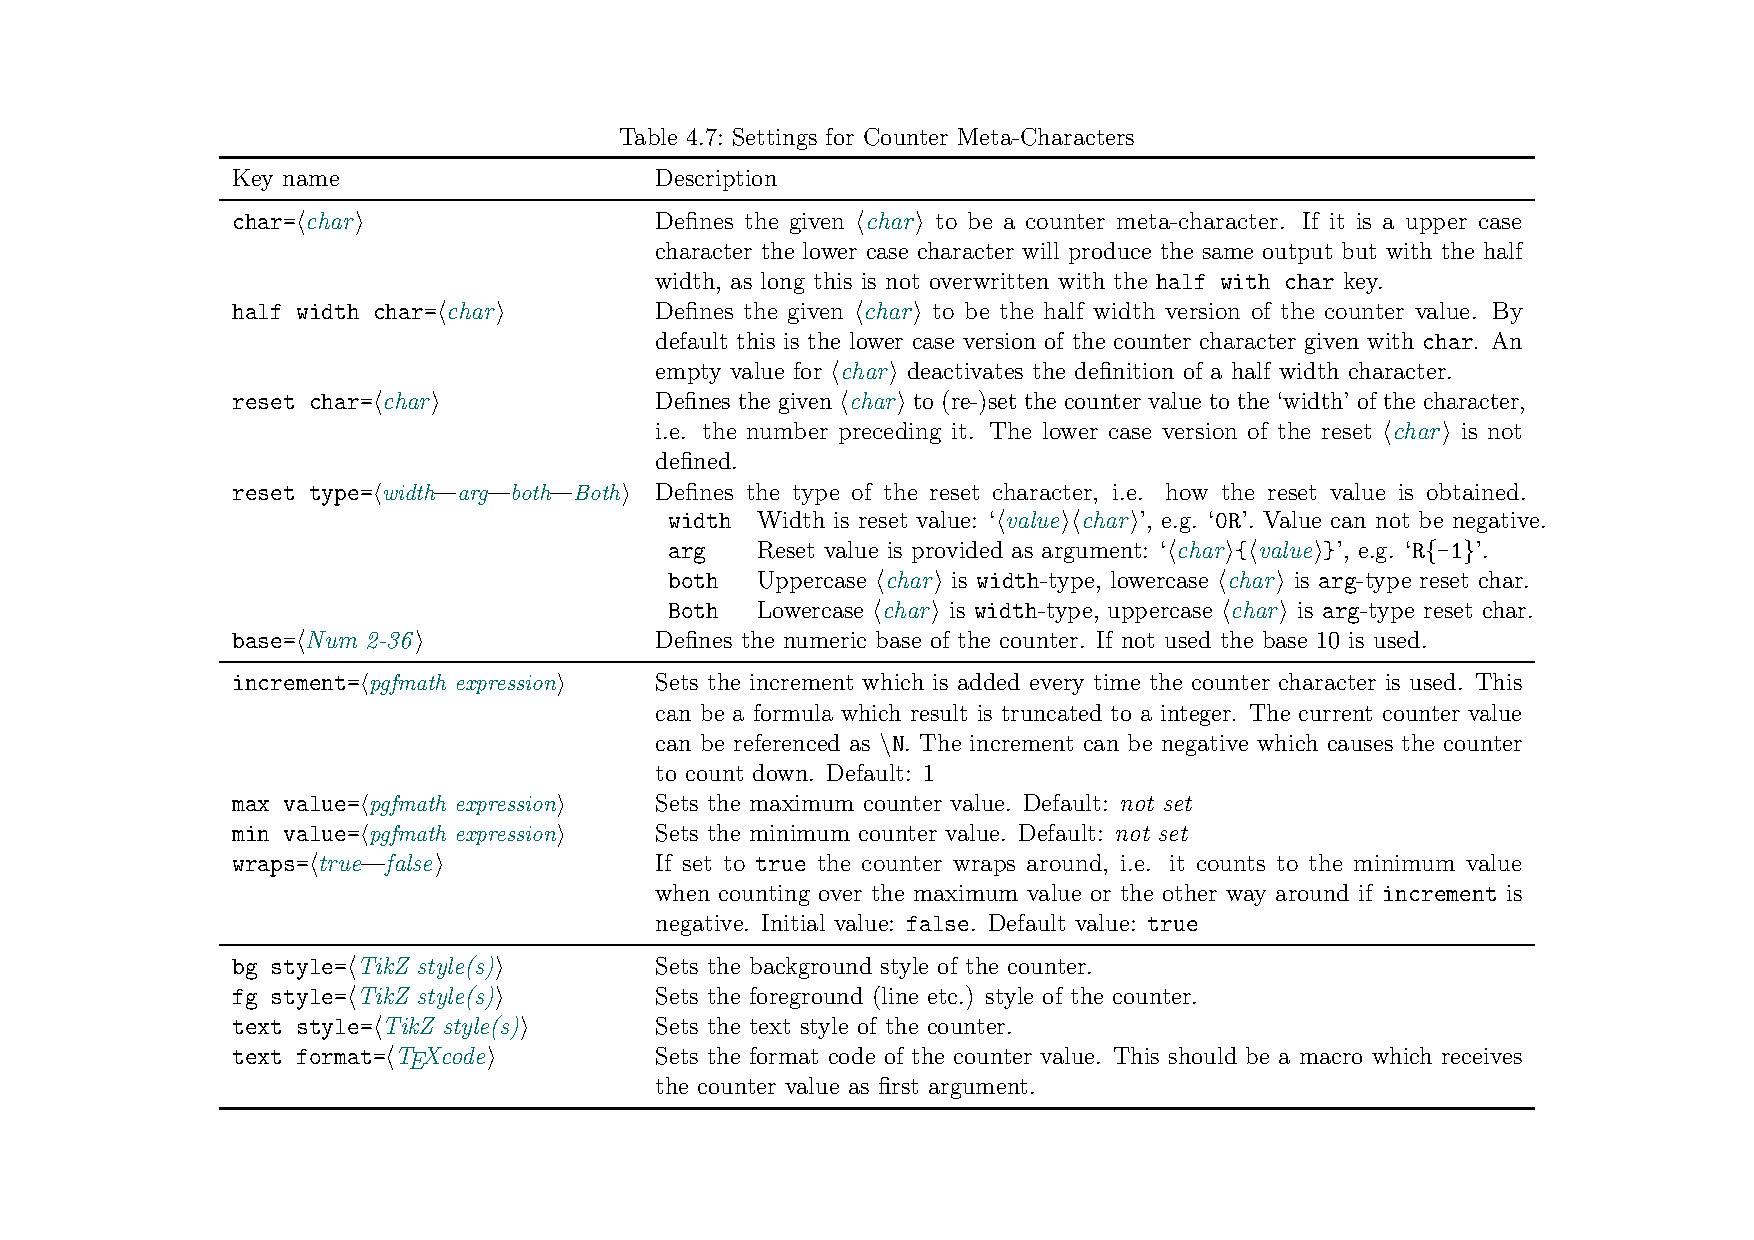
\includegraphics[width=14cm]{tikz-timing/tikz-timing-var_meta}\\
\end{table}

\begin{table}[H]
  \centering
  \caption{tikz-timing-modifier 参数表}\label{tikz-timing-var_modifier}
  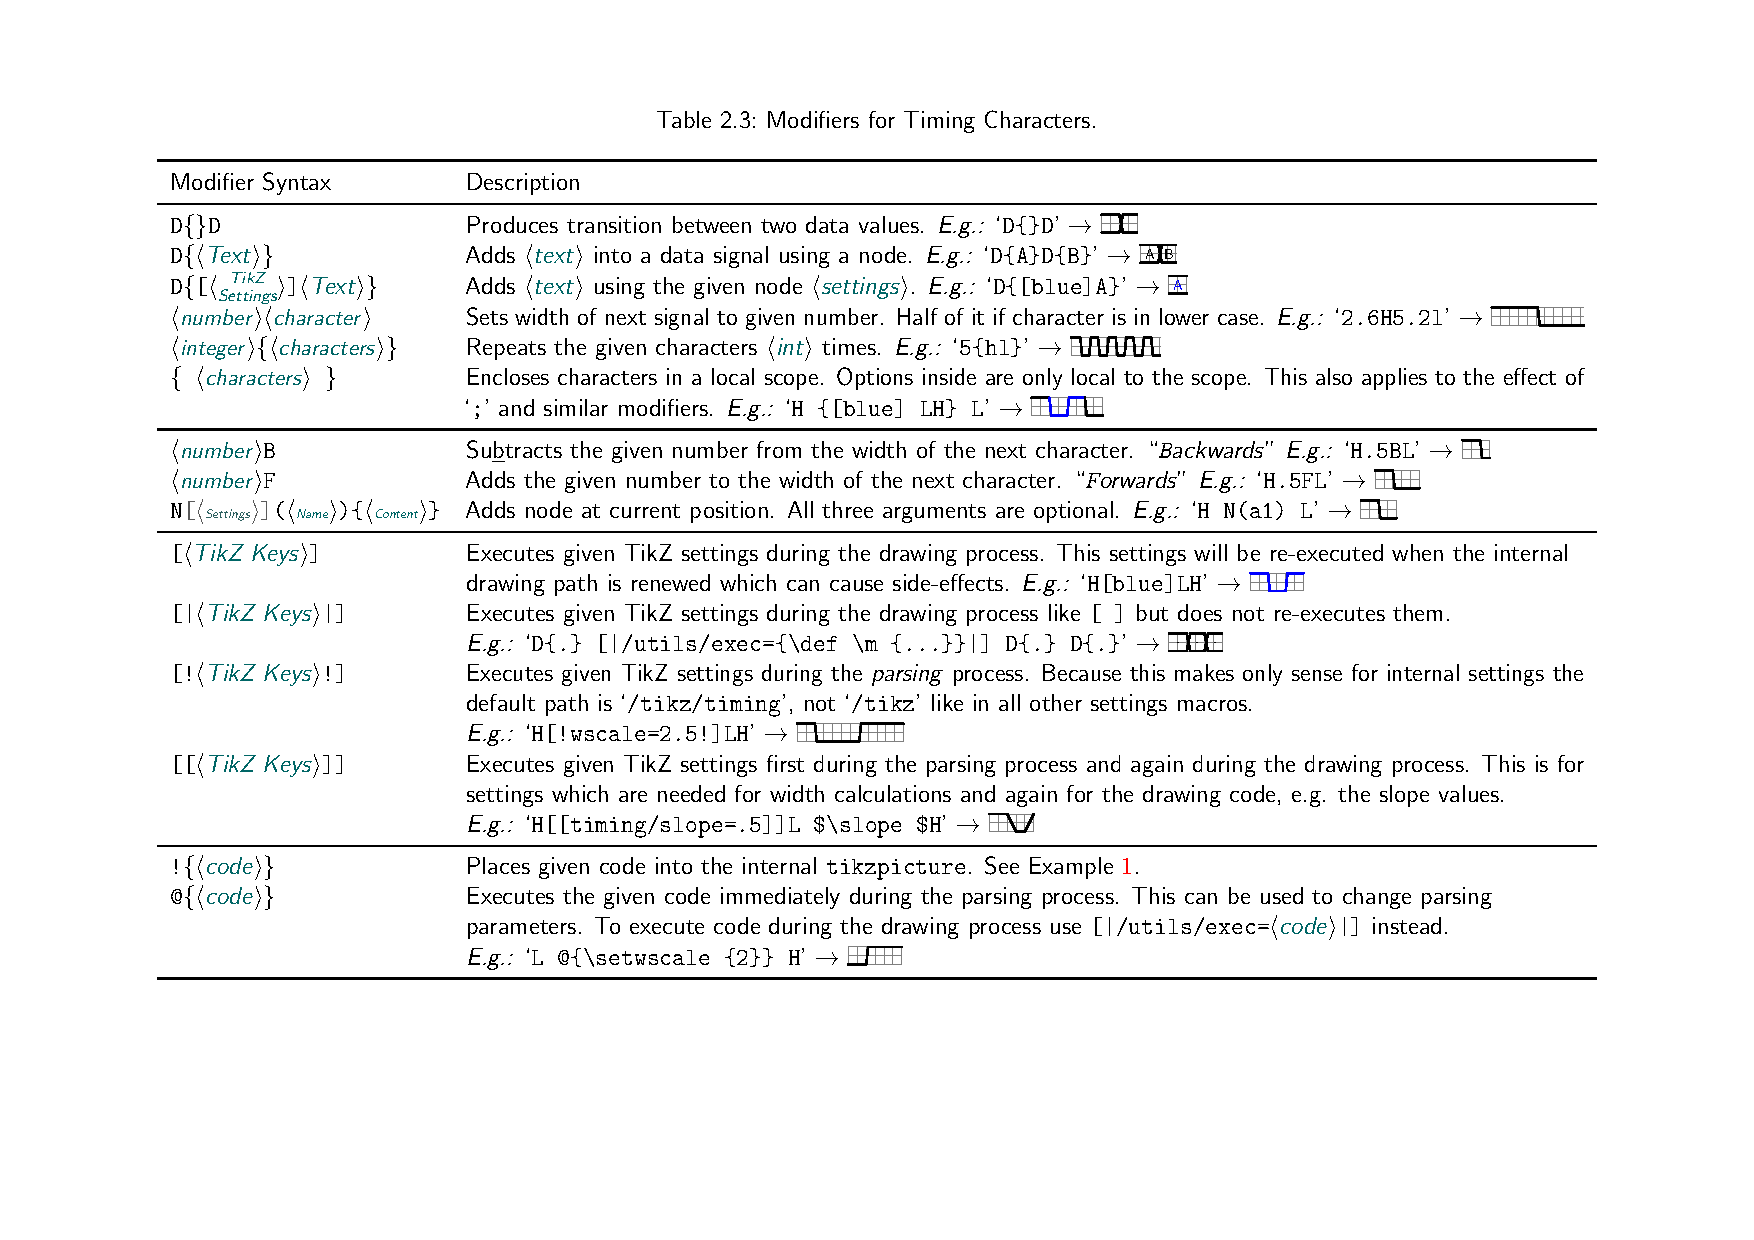
\includegraphics[width=14cm]{tikz-timing/tikz-timing-var_modifier}\\
\end{table}

\begin{table}[H]
  \centering
  \caption{tikz-timing-modifier 参数表2}\label{tikz-timing-var_modifier2}
  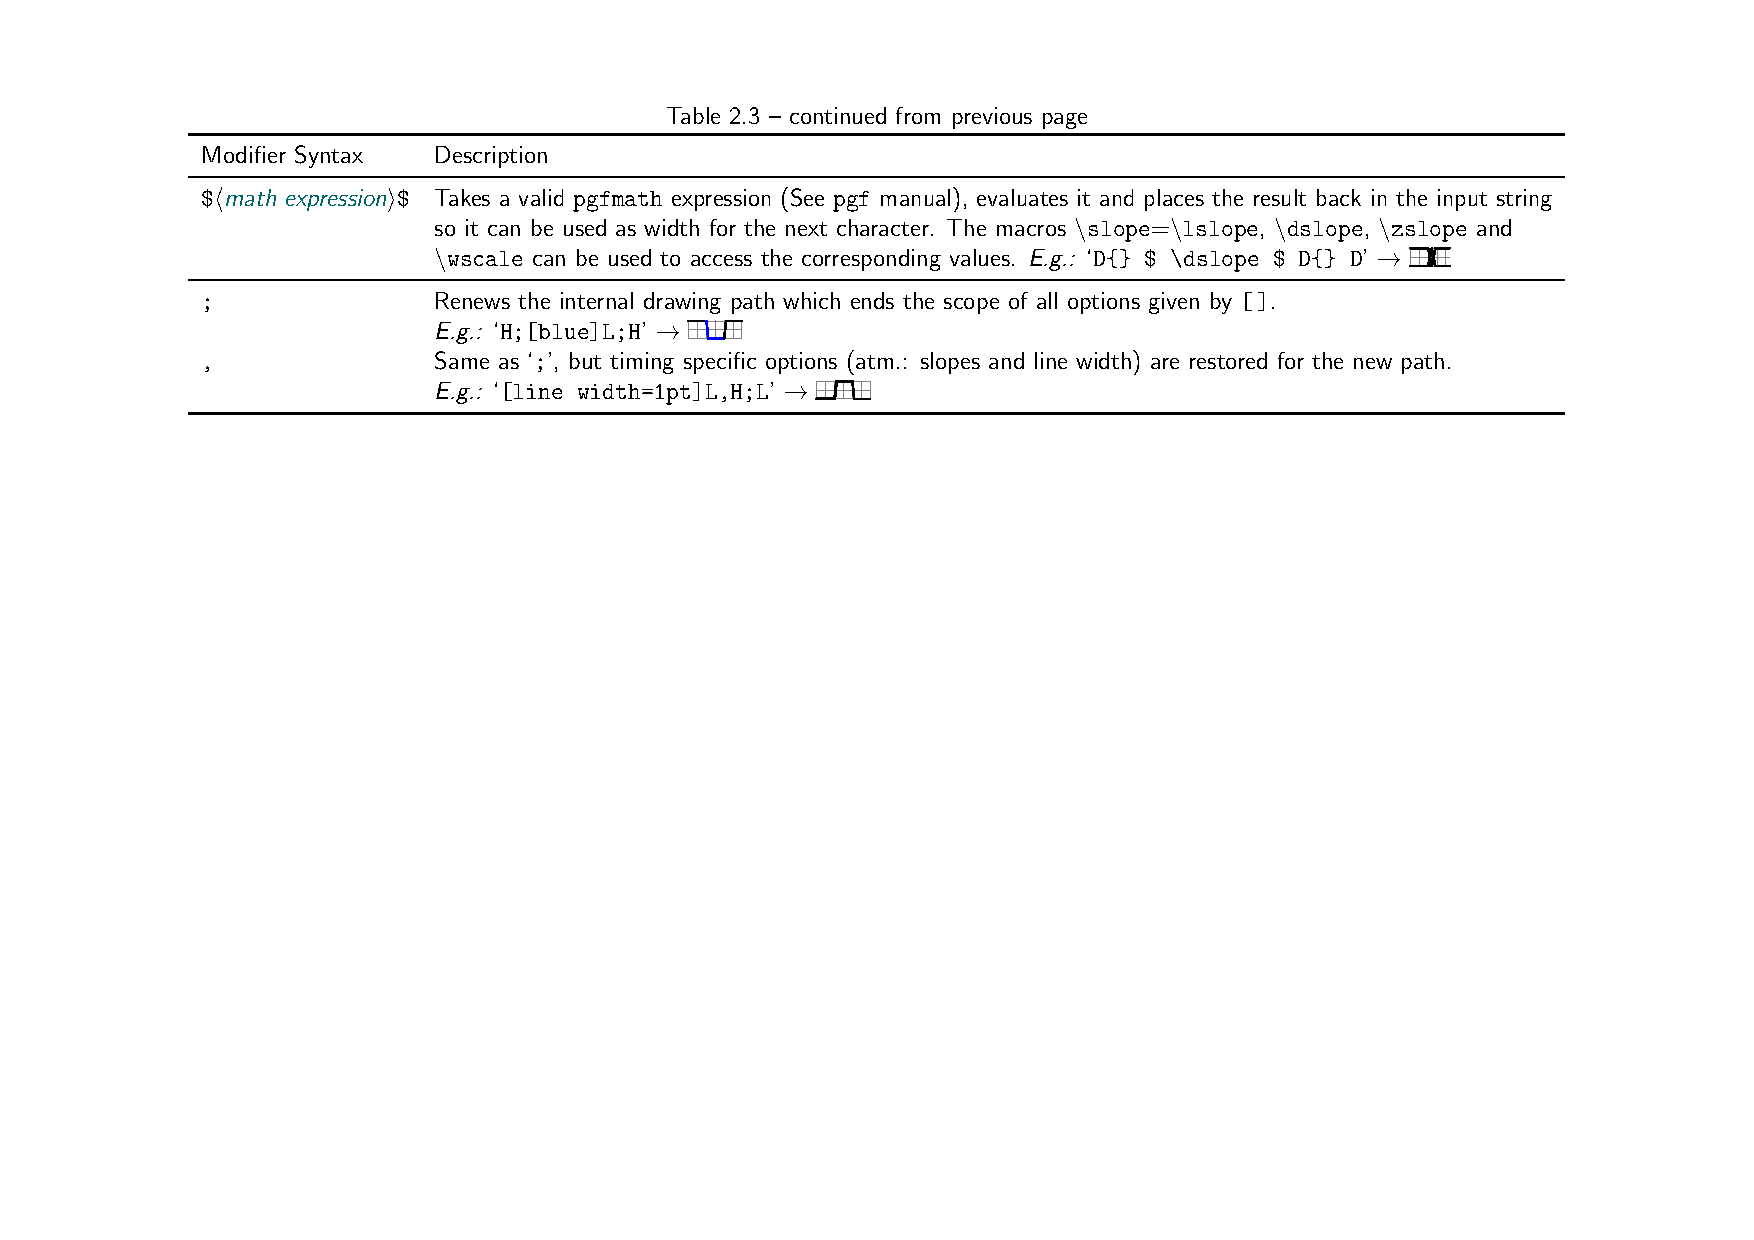
\includegraphics[width=14cm]{tikz-timing/tikz-timing-var_modifier2}\\
\end{table}



\begin{table}[H]
  \centering
  % Requires \usepackage{graphicx}
  \caption{tikz-timing-setting 参数表}
  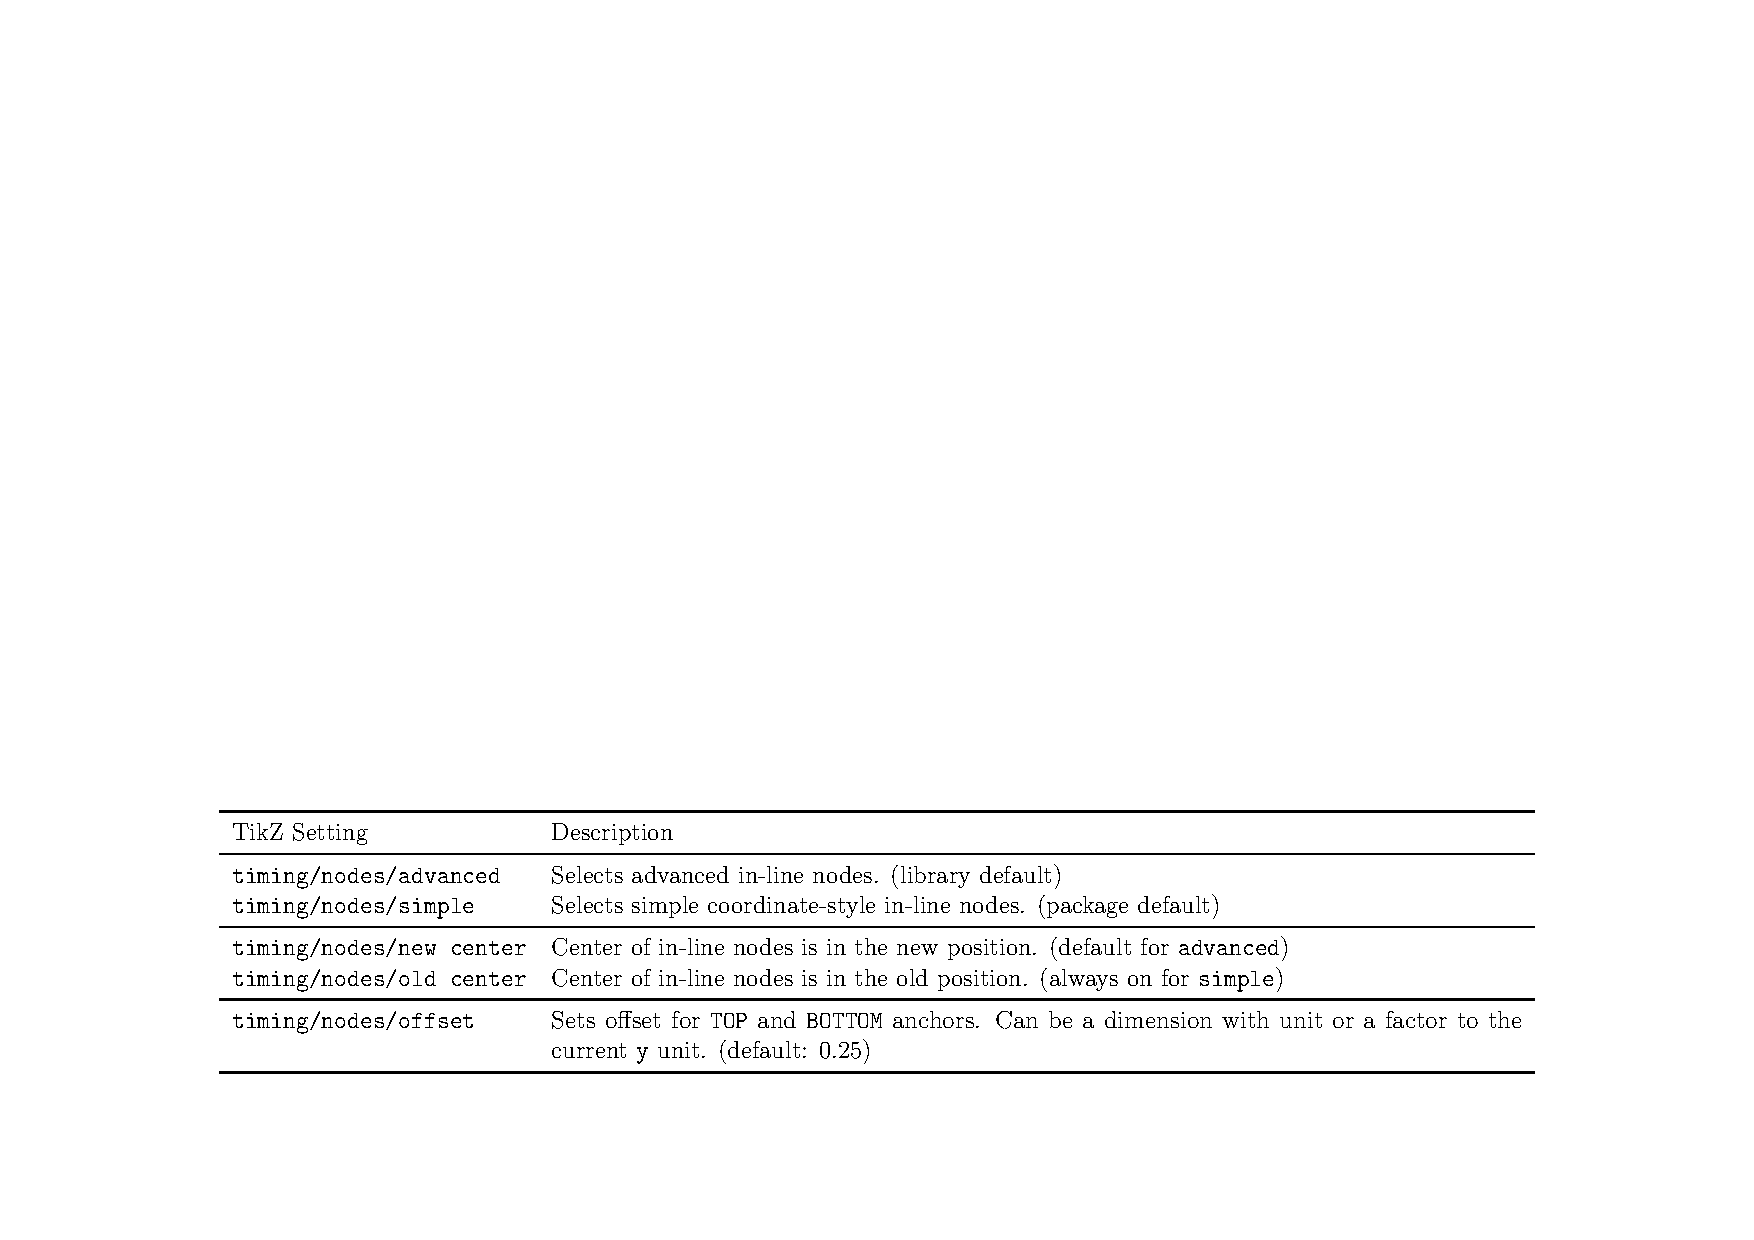
\includegraphics[width=14cm]{tikz-timing/tikz-timing-var_setting}\\
  
  \label{tikz-timing-var_setting}
\end{table}
\begin{table}[H]
  \centering
  % Requires \usepackage{graphicx}
   \caption{tikz-timing-general-slope-text 参数表}
  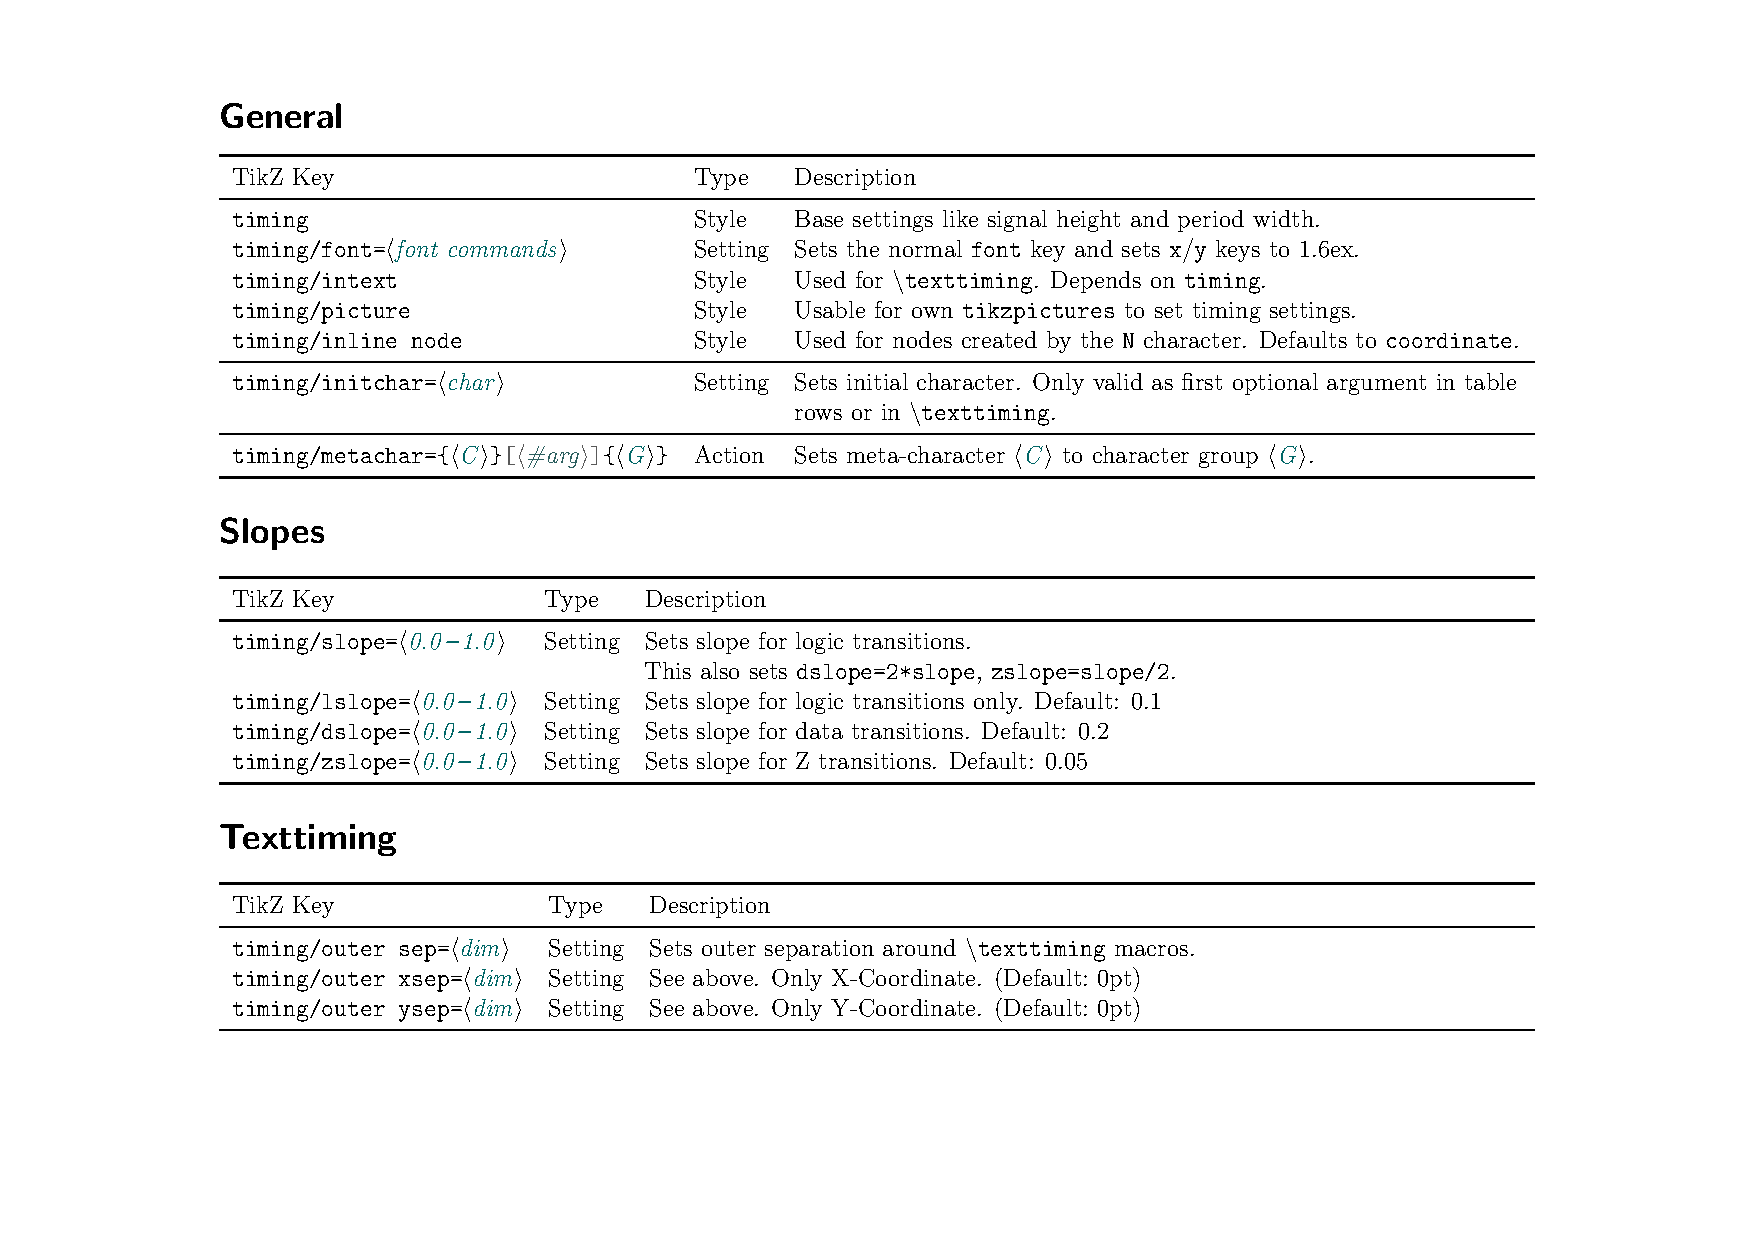
\includegraphics[width=14cm]{tikz-timing/tikz-timing-var_slope_text}\\
 
  \label{tikz-timing-var_slope_text}
\end{table}

\begin{figure}[H]
  \centering
  % Requires \usepackage{graphicx}
  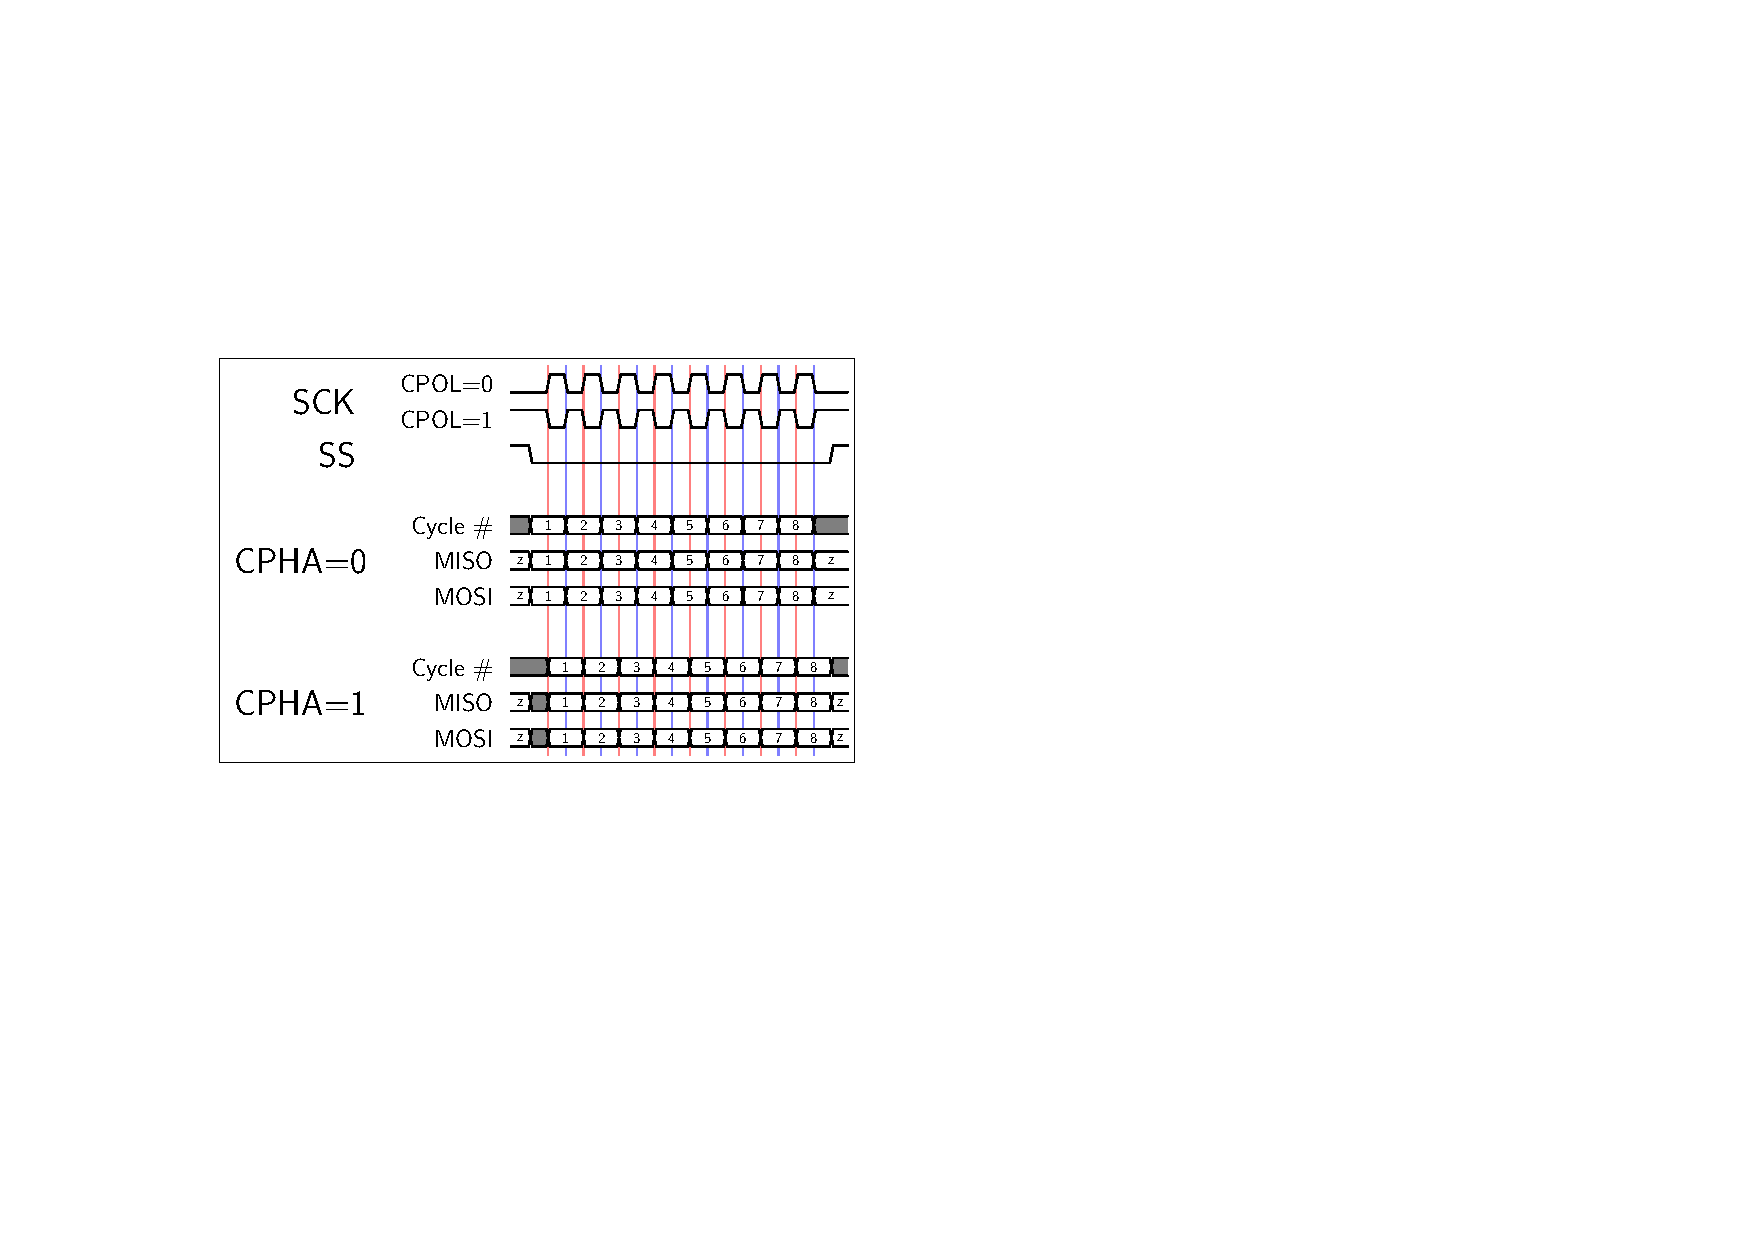
\includegraphics[width=14cm]{tikz-timing/tikz-timing-var_spi}\\
  \caption{tikz-timing-SPI 时序图}
  \label{tikz-timing-var_spi}
\end{figure}



\noindent\verb|\texttiming{HLZDZLH}|: \texttiming{HLZDZLH}\\
\verb|\texttiming[green,timing/initchar=L]{HLZDZLH}|: \texttiming[green,timing/initchar=L]{HLZDZLH}
\begin{figure}[H]
  \centering
\begin{tikztimingtable}
Clock 128\,MHz 0\degr & H 2C N(A1) 8{2C} N(A5) 3{2C} G\\
Clock 128\,MHz 90\degr & [C] 2{2C} N(A2) 8{2C} N(A6) 2{2C} C\\
Clock 128\,MHz 180\degr & C 2{2C} N(A3) 8{2C} N(A7) 2{2C} G\\
Clock 128\,MHz 270\degr & 3{2C} N(A4) 8{2C} N(A8) 2C C\\
Coarse Pulse & 3L 16H 6L \\
Coarse Pulse - Delayed 1 & 4L N(B2) 16H N(B6) 5L \\
Coarse Pulse - Delayed 2 & 5L N(B3) 16H N(B7) 4L \\
Coarse Pulse - Delayed 3 & 6L 16H 3L \\
\\
Final Pulse Set & 3L 16H N(B5) 6L \\
Final Pulse $\overline{\mbox{Reset}}$ & 6L N(B4) 16H 3L \\
Final Pulse & 3L N(B1) 19H N(B8) 3L \\
\extracode
\tablerules
\begin{pgfonlayer}{background}
\foreach \n in {1,...,8}
\draw [help lines] (A\n) -- (B\n);
\end{pgfonlayer}
\end{tikztimingtable}
 \caption{时序图pgf}\label{pgf_timing}
\end{figure}

\begin{lstlisting}
\begin{figure}[H]
  \centering
\begin{tikztimingtable}
Clock 128\,MHz 0\degr & H 2C N(A1) 8{2C} N(A5) 3{2C} G\\
Clock 128\,MHz 90\degr & [C] 2{2C} N(A2) 8{2C} N(A6) 2{2C} C\\
Clock 128\,MHz 180\degr & C 2{2C} N(A3) 8{2C} N(A7) 2{2C} G\\
Clock 128\,MHz 270\degr & 3{2C} N(A4) 8{2C} N(A8) 2C C\\
Coarse Pulse & 3L 16H 6L \\
Coarse Pulse - Delayed 1 & 4L N(B2) 16H N(B6) 5L \\
Coarse Pulse - Delayed 2 & 5L N(B3) 16H N(B7) 4L \\
Coarse Pulse - Delayed 3 & 6L 16H 3L \\
\\
Final Pulse Set & 3L 16H N(B5) 6L \\
Final Pulse $\overline{\mbox{Reset}}$ & 6L N(B4) 16H 3L \\
Final Pulse & 3L N(B1) 19H N(B8) 3L \\
\extracode
\tablerules
\begin{pgfonlayer}{background}
\foreach \n in {1,...,8}
\draw [help lines] (A\n) -- (B\n);
\end{pgfonlayer}
\end{tikztimingtable}
 \caption{`时序图`pgf}\label{pgf_timing}
\end{figure}
\end{lstlisting}

\tikzexternalenable

\section{circuitikz 电路图}
\tikzexternaldisable
\subsection{绘制命令参数}
\begin{cmd}[label= circuitikz绘制命令参数]
\begin{circuitikz}[scale=比例因子]
\draw (起始点坐标) [R,参数赋值] (结束点坐标)
参数有l=(label,显示出R的标号),
i^>=;i_>=;i^<=;i<^=;电流
[american voltages] 可选项显示为正负
[european voltages] 可选项显示为弧形箭头
v^>=;v_>=;v_<=;v^<=;电压
o-*;o-o;*-*;*-o;*-;o-;显示两端黑白结点
anchor=north,south,west,east 其中之一或组合,指定文本排放的相对位置
\end{cmd}

调用 circuitikz 宏包和 tikzlibaray 中的以下自带宏包。
\begin{itemize}
  \item shapes.gates.logic.US,
  \item shapes.gates.logic.IEC,
  \item circuits.logic.US,
  \item circuits.logic.IEC,
  \item circuits.logic.CDH,
  \item circuits.ee.IEC,
\end{itemize}


\subsection{逻辑门绘制}
有 IEC,US,CDH 三种标准,如\ref{logic_table}所示
\newcommand{\gateexamples}[1]{%
  %\texttt{#1}
  %\indexkey{#1}&
  #1 &
  \tikz[baseline,circuit logic IEC] \node[#1,label=] {}; &
  \tikz[baseline,circuit logic US]  \node[#1] {}; &
  \tikz[baseline,circuit logic CDH] \node[#1] {};
}

\begin{table}[H]
  \centering
  \caption{逻辑门三种表示方式}\label{logic_table}
\rowcolors{1}{lightgray}{}
\begin{tabular}{lccc}
\toprule
  \emph{Key} & \emph{Appearance inside} & \emph{Appearance inside} & \emph{Appearance inside} \\
      & |circuit logic IEC| & |circuit logic US| & |circuit logic CDH| \\
\midrule
  \gateexamples{/tikz/and gate}\\
  \gateexamples{/tikz/nand gate}\\
  \gateexamples{/tikz/or gate}\\
  \gateexamples{/tikz/nor gate}\\
  \gateexamples{/tikz/xor gate}\\
  \gateexamples{/tikz/xnor gate}\\
  \gateexamples{/tikz/not gate}\\
  \gateexamples{/tikz/buffer gate}\\
\bottomrule
\end{tabular}
\end{table}

\subsection{元器件:电阻、电感、电容、电池、变压器}
绘制代码:
\begin{cmd}
\draw(x坐标,y坐标) node[元器件代码,元器件属性赋值] (元器件代号) {显示名称}
\end{cmd}

\begin{minipage}[c]{2.5cm}
\begin{circuitikz} \draw
  (0,0) node[pnp, color=blue] (pnp2) {}
  (pnp2.B) node[pnp, xscale=-1, anchor=B, color=brown] (pnp1) {}
  (pnp1.C) node[npn, anchor=C, color=green] (npn1) {}
  (pnp2.C) node[npn, xscale=-1, anchor=C, color=magenta] (npn2) {}
  (pnp1.E) -- (pnp2.E)  (npn1.E) -- (npn2.E)
  (pnp1.B) node[circ] {} |- (pnp2.C) node[circ] {}
;\end{circuitikz}
\end{minipage}
\begin{minipage}[c]{9.5cm}
 \begin{lstlisting}
\begin{circuitikz} \draw
  (0,0) node[pnp, color=blue] (pnp2) {}
  (pnp2.B) node[pnp, xscale=-1, anchor=B, color=brown] (pnp1) {}
  (pnp1.C) node[npn, anchor=C, color=green] (npn1) {}
  (pnp2.C) node[npn, xscale=-1, anchor=C, color=magenta] (npn2) {}
  (pnp1.E) -- (pnp2.E)
  (npn1.E) -- (npn2.E)
  (pnp1.B) node[circ] {} |- (pnp2.C) node[circ] {}
;\end{circuitikz}
\end{lstlisting}
\end{minipage}




\begin{minipage}[c]{1.5cm}

\begin{circuitikz}
   \draw (0,0) to[R, l=$R_1$] (2,0);
\end{circuitikz}

\end{minipage}
\begin{minipage}[c]{13cm}
 \begin{lstlisting}

\begin{circuitikz}
   \draw (0,0) to[R, l=$R_1$] (2,0);
\end{circuitikz}

\end{lstlisting}
\end{minipage}





\begin{minipage}[c]{1.5cm}
\begin{circuitikz}
   \draw (0,0) to[R=$R_1$] (2,0);
\end{circuitikz}

\end{minipage}
\begin{minipage}[c]{13cm}
 \begin{lstlisting}
\begin{circuitikz}
   \draw (0,0) to[R=$R_1$] (2,0);
\end{circuitikz}

\end{lstlisting}
\end{minipage}





\begin{minipage}[c]{1.5cm}
\begin{circuitikz}
   \draw (0,0) to[R, i=$i_1$] (2,0);
\end{circuitikz}

\end{minipage}
\begin{minipage}[c]{13cm}
 \begin{lstlisting}
\begin{circuitikz}
   \draw (0,0) to[R, i=$i_1$] (2,0);
\end{circuitikz}

\end{lstlisting}
\end{minipage}



\begin{minipage}[c]{1.5cm}
\begin{circuitikz}
   \draw (0,0) to[R, v=$v_1$] (2,0);
\end{circuitikz}

\end{minipage}
\begin{minipage}[c]{13cm}
 \begin{lstlisting}
\begin{circuitikz}
   \draw (0,0) to[R, v=$v_1$] (2,0);
\end{circuitikz}

\end{lstlisting}
\end{minipage}





\begin{minipage}[c]{1.5cm}
\begin{circuitikz}
   \draw (0,0) to[R=$R_1$, i=$i_1$, v=$v_1$] (2,0);
\end{circuitikz}

\end{minipage}
\begin{minipage}[c]{13cm}
 \begin{lstlisting}
\begin{circuitikz}
   \draw (0,0) to[R=$R_1$, i=$i_1$, v=$v_1$] (2,0);
\end{circuitikz}

\end{lstlisting}
\end{minipage}



\begin{minipage}[c]{1.5cm}
\begin{circuitikz}
   \draw (0,0) to[R=$R_1$, i=$i_1$, v=$v_1$] (2,0);
\end{circuitikz}

\end{minipage}
\begin{minipage}[c]{13cm}
 \begin{lstlisting}
\begin{circuitikz}
   \draw (0,0) to[R=$R_1$, i=$i_1$, v=$v_1$] (2,0);
\end{circuitikz}

\end{lstlisting}
\end{minipage}



\subsection{标注}


\begin{minipage}[c]{3.5cm}

\begin{circuitikz}
   \draw (0,0) to[R, l^=$R_1$] (2,0);
\end{circuitikz}

\end{minipage}
\begin{minipage}[c]{10cm}
 \begin{lstlisting}

\begin{circuitikz}
   \draw (0,0) to[R, l^=$R_1$] (2,0);
\end{circuitikz}

\end{lstlisting}
\end{minipage}




\begin{minipage}[c]{1.5cm}

\begin{circuitikz}
   \draw (0,0) to[R, l_=$R_1$] (2,0);
\end{circuitikz}

\end{minipage}
\begin{minipage}[c]{13cm}
 \begin{lstlisting}

\begin{circuitikz}
   \draw (0,0) to[R, l_=$R_1$] (2,0);
\end{circuitikz}

\end{lstlisting}
\end{minipage}



\noindent The default orientation of labels is controlled by the options \texttt{smartlabels}, \texttt{rotatelabels} and \texttt{straightlabels} (or the corresponding \texttt{label/align} keys). Here are examples to see the differences:


\begin{minipage}[c]{4.5cm}
\begin{circuitikz}
\ctikzset{label/align = straight}
\def\DIR{0,45,90,135,180,-90,-45,-135}
\foreach \i in \DIR {
  \draw (0,0) to[R=\i, *-o] (\i:2.5);
}
\end{circuitikz}
\end{minipage}
\begin{minipage}[c]{11cm}
 \begin{lstlisting}
\begin{circuitikz}
\ctikzset{label/align = straight}
\def\DIR{0,45,90,135,180,-90,-45,-135}
\foreach \i in \DIR {
  \draw (0,0) to[R=\i, *-o] (\i:2.5);
}
\end{circuitikz}
\end{lstlisting}
\end{minipage}




\begin{minipage}[c]{4.5cm}
\begin{circuitikz}
\ctikzset{label/align = rotate}
\def\DIR{0,45,90,135,180,-90,-45,-135}
\foreach \i in \DIR {
  \draw (0,0) to[R=\i, *-o] (\i:2.5);
}
\end{circuitikz}
\end{minipage}
\begin{minipage}[c]{11cm}
 \begin{lstlisting}
\begin{circuitikz}
\ctikzset{label/align = rotate}
\def\DIR{0,45,90,135,180,-90,-45,-135}
\foreach \i in \DIR {
  \draw (0,0) to[R=\i, *-o] (\i:2.5);
}
\end{circuitikz}
\end{lstlisting}
\end{minipage}


\begin{minipage}[c]{4.5cm}
\begin{circuitikz}
\ctikzset{label/align = smart}
\def\DIR{0,45,90,135,180,-90,-45,-135}
\foreach \i in \DIR {
  \draw (0,0) to[R=\i, *-o] (\i:2.5);
}
\end{circuitikz}
\end{minipage}
\begin{minipage}[c]{11cm}
 \begin{lstlisting}
\begin{circuitikz}
\ctikzset{label/align = smart}
\def\DIR{0,45,90,135,180,-90,-45,-135}
\foreach \i in \DIR {
  \draw (0,0) to[R=\i, *-o] (\i:2.5);
}
\end{circuitikz}
\end{lstlisting}
\end{minipage}



\subsection{电流}


\begin{minipage}[c]{1.5cm}

\begin{circuitikz}
   \draw (0,0) to[R, i^>=$i_1$] (2,0);
\end{circuitikz}
\end{minipage}
\begin{minipage}[c]{13cm}
 \begin{lstlisting}

\begin{circuitikz}
   \draw (0,0) to[R, i^>=$i_1$] (2,0);
\end{circuitikz}
\end{lstlisting}
\end{minipage}




\begin{minipage}[c]{1.5cm}
\begin{circuitikz}
   \draw (0,0) to[R, i_>=$i_1$] (2,0);
\end{circuitikz}
\end{minipage}
\begin{minipage}[c]{13cm}
 \begin{lstlisting}
\begin{circuitikz}
   \draw (0,0) to[R, i_>=$i_1$] (2,0);
\end{circuitikz}
\end{lstlisting}
\end{minipage}





\begin{minipage}[c]{1.5cm}
\begin{circuitikz}
   \draw (0,0) to[R, i^<=$i_1$] (2,0);
\end{circuitikz}
\end{minipage}
\begin{minipage}[c]{13cm}
 \begin{lstlisting}
\begin{circuitikz}
   \draw (0,0) to[R, i^<=$i_1$] (2,0);
\end{circuitikz}
\end{lstlisting}
\end{minipage}





\begin{minipage}[c]{1.5cm}
\begin{circuitikz}
   \draw (0,0) to[R, i_<=$i_1$] (2,0);
\end{circuitikz}
\end{minipage}
\begin{minipage}[c]{13cm}
 \begin{lstlisting}
\begin{circuitikz}
   \draw (0,0) to[R, i_<=$i_1$] (2,0);
\end{circuitikz}
\end{lstlisting}
\end{minipage}





\begin{minipage}[c]{1.5cm}
\begin{circuitikz}
   \draw (0,0) to[R, i>^=$i_1$] (2,0);
\end{circuitikz}
\end{minipage}
\begin{minipage}[c]{13cm}
 \begin{lstlisting}
\begin{circuitikz}
   \draw (0,0) to[R, i>^=$i_1$] (2,0);
\end{circuitikz}
\end{lstlisting}
\end{minipage}





\begin{minipage}[c]{1.5cm}
\begin{circuitikz}
   \draw (0,0) to[R, i>_=$i_1$] (2,0);
\end{circuitikz}
\end{minipage}
\begin{minipage}[c]{13cm}
 \begin{lstlisting}
\begin{circuitikz}
   \draw (0,0) to[R, i>_=$i_1$] (2,0);
\end{circuitikz}
\end{lstlisting}
\end{minipage}





\begin{minipage}[c]{1.5cm}
\begin{circuitikz}
   \draw (0,0) to[R, i<^=$i_1$] (2,0);
\end{circuitikz}
\end{minipage}
\begin{minipage}[c]{13cm}
 \begin{lstlisting}
\begin{circuitikz}
   \draw (0,0) to[R, i<^=$i_1$] (2,0);
\end{circuitikz}
\end{lstlisting}
\end{minipage}





\begin{minipage}[c]{1.5cm}
\begin{circuitikz}
   \draw (0,0) to[R, i<_=$i_1$] (2,0);
\end{circuitikz}
\end{minipage}
\begin{minipage}[c]{13cm}
 \begin{lstlisting}
\begin{circuitikz}
   \draw (0,0) to[R, i<_=$i_1$] (2,0);
\end{circuitikz}
\end{lstlisting}
\end{minipage}





Also

\begin{minipage}[c]{1.5cm}
\begin{circuitikz}
   \draw (0,0) to[R, i<=$i_1$] (2,0);
\end{circuitikz}
\end{minipage}
\begin{minipage}[c]{13cm}
 \begin{lstlisting}
\begin{circuitikz}
   \draw (0,0) to[R, i<=$i_1$] (2,0);
\end{circuitikz}
\end{lstlisting}
\end{minipage}





\begin{minipage}[c]{1.5cm}
\begin{circuitikz}
   \draw (0,0) to[R, i>=$i_1$] (2,0);
\end{circuitikz}
\end{minipage}
\begin{minipage}[c]{13cm}
 \begin{lstlisting}
\begin{circuitikz}
   \draw (0,0) to[R, i>=$i_1$] (2,0);
\end{circuitikz}
\end{lstlisting}
\end{minipage}





\begin{minipage}[c]{1.5cm}
\begin{circuitikz}
   \draw (0,0) to[R, i^=$i_1$] (2,0);
\end{circuitikz}
\end{minipage}
\begin{minipage}[c]{13cm}
 \begin{lstlisting}
\begin{circuitikz}
   \draw (0,0) to[R, i^=$i_1$] (2,0);
\end{circuitikz}
\end{lstlisting}
\end{minipage}





\begin{minipage}[c]{1.5cm}
\begin{circuitikz}
   \draw (0,0) to[R, i_=$i_1$] (2,0);
\end{circuitikz}

\end{minipage}
\begin{minipage}[c]{13cm}
 \begin{lstlisting}
\begin{circuitikz}
   \draw (0,0) to[R, i_=$i_1$] (2,0);
\end{circuitikz}

\end{lstlisting}
\end{minipage}






\subsection{电压}

\subsubsection{European style} The default, with arrows. Use option \texttt{europeanvoltage} or style \verb![european voltages]!.


\begin{minipage}[c]{1.5cm}
\begin{circuitikz}[european voltages]
   \draw (0,0) to[R, v^>=$v_1$] (2,0);
\end{circuitikz}
\end{minipage}
\begin{minipage}[c]{13cm}
 \begin{lstlisting}
\begin{circuitikz}[european voltages]
   \draw (0,0) to[R, v^>=$v_1$] (2,0);
\end{circuitikz}
\end{lstlisting}
\end{minipage}




\begin{minipage}[c]{1.5cm}
\begin{circuitikz}[european voltages]
   \draw (0,0) to[R, v^<=$v_1$] (2,0);
\end{circuitikz}
\end{minipage}
\begin{minipage}[c]{13cm}
 \begin{lstlisting}
\begin{circuitikz}[european voltages]
   \draw (0,0) to[R, v^<=$v_1$] (2,0);
\end{circuitikz}
\end{lstlisting}
\end{minipage}





\begin{minipage}[c]{1.5cm}
\begin{circuitikz}[european voltages]
   \draw (0,0) to[R, v_>=$v_1$] (2,0);
\end{circuitikz}
\end{minipage}
\begin{minipage}[c]{13cm}
 \begin{lstlisting}
\begin{circuitikz}[european voltages]
   \draw (0,0) to[R, v_>=$v_1$] (2,0);
\end{circuitikz}
\end{lstlisting}
\end{minipage}





\begin{minipage}[c]{1.5cm}
\begin{circuitikz}[european voltages]
   \draw (0,0) to[R, v_<=$v_1$] (2,0);
\end{circuitikz}
\end{minipage}
\begin{minipage}[c]{13cm}
 \begin{lstlisting}
\begin{circuitikz}[european voltages]
   \draw (0,0) to[R, v_<=$v_1$] (2,0);
\end{circuitikz}
\end{lstlisting}
\end{minipage}





\subsubsection{American style} For those who like it (not me). Use option \texttt{americanvoltage} or set \verb![american voltages]!.

\begin{minipage}[c]{1.5cm}
\begin{circuitikz}[american voltages]
   \draw (0,0) to[R, v^>=$v_1$] (2,0);
\end{circuitikz}
\end{minipage}
\begin{minipage}[c]{13cm}
 \begin{lstlisting}
\begin{circuitikz}[american voltages]
   \draw (0,0) to[R, v^>=$v_1$] (2,0);
\end{circuitikz}
\end{lstlisting}
\end{minipage}





\begin{minipage}[c]{1.5cm}
\begin{circuitikz}[american voltages]
   \draw (0,0) to[R, v^<=$v_1$] (2,0);
\end{circuitikz}
\end{minipage}
\begin{minipage}[c]{13cm}
 \begin{lstlisting}
\begin{circuitikz}[american voltages]
   \draw (0,0) to[R, v^<=$v_1$] (2,0);
\end{circuitikz}
\end{lstlisting}
\end{minipage}





\begin{minipage}[c]{1.5cm}
\begin{circuitikz}[american voltages]
   \draw (0,0) to[R, v_>=$v_1$] (2,0);
\end{circuitikz}
\end{minipage}
\begin{minipage}[c]{13cm}
 \begin{lstlisting}
\begin{circuitikz}[american voltages]
   \draw (0,0) to[R, v_>=$v_1$] (2,0);
\end{circuitikz}
\end{lstlisting}
\end{minipage}





\begin{minipage}[c]{1.5cm}
\begin{circuitikz}[american voltages]
   \draw (0,0) to[R, v_<=$v_1$] (2,0);
\end{circuitikz}
\end{minipage}
\begin{minipage}[c]{13cm}
 \begin{lstlisting}
\begin{circuitikz}[american voltages]
   \draw (0,0) to[R, v_<=$v_1$] (2,0);
\end{circuitikz}
\end{lstlisting}
\end{minipage}







\subsection{结点}


\begin{minipage}[c]{1.5cm}
\begin{circuitikz}
   \draw (0,0) to[R, o-o] (2,0);
\end{circuitikz}
\end{minipage}
\begin{minipage}[c]{13cm}
 \begin{lstlisting}
\begin{circuitikz}
   \draw (0,0) to[R, o-o] (2,0);
\end{circuitikz}
\end{lstlisting}
\end{minipage}




\begin{minipage}[c]{1.5cm}
\begin{circuitikz}
   \draw (0,0) to[R, -o] (2,0);
\end{circuitikz}
\end{minipage}
\begin{minipage}[c]{13cm}
 \begin{lstlisting}
\begin{circuitikz}
   \draw (0,0) to[R, -o] (2,0);
\end{circuitikz}
\end{lstlisting}
\end{minipage}





\begin{minipage}[c]{1.5cm}
\begin{circuitikz}
   \draw (0,0) to[R, o-] (2,0);
\end{circuitikz}
\end{minipage}
\begin{minipage}[c]{13cm}
 \begin{lstlisting}
\begin{circuitikz}
   \draw (0,0) to[R, o-] (2,0);
\end{circuitikz}
\end{lstlisting}
\end{minipage}





\begin{minipage}[c]{1.5cm}
\begin{circuitikz}
   \draw (0,0) to[R, *-*] (2,0);
\end{circuitikz}
\end{minipage}
\begin{minipage}[c]{13cm}
 \begin{lstlisting}
\begin{circuitikz}
   \draw (0,0) to[R, *-*] (2,0);
\end{circuitikz}
\end{lstlisting}
\end{minipage}






\begin{minipage}[c]{1.5cm}
\begin{circuitikz}
   \draw (0,0) to[R, -*] (2,0);
\end{circuitikz}

\end{minipage}
\begin{minipage}[c]{13cm}
 \begin{lstlisting}
\begin{circuitikz}
   \draw (0,0) to[R, -*] (2,0);
\end{circuitikz}

\end{lstlisting}
\end{minipage}



\begin{minipage}[c]{1.5cm}
\begin{circuitikz}
   \draw (0,0) to[R, *-] (2,0);
\end{circuitikz}
\end{minipage}
\begin{minipage}[c]{13cm}
 \begin{lstlisting}
\begin{circuitikz}
   \draw (0,0) to[R, *-] (2,0);
\end{circuitikz}
\end{lstlisting}
\end{minipage}





\begin{minipage}[c]{1.5cm}
\begin{circuitikz}
   \draw (0,0) to[R, o-*] (2,0);
\end{circuitikz}
\end{minipage}
\begin{minipage}[c]{13cm}
 \begin{lstlisting}
\begin{circuitikz}
   \draw (0,0) to[R, o-*] (2,0);
\end{circuitikz}
\end{lstlisting}
\end{minipage}





\begin{minipage}[c]{1.5cm}
\begin{circuitikz}
   \draw (0,0) to[R, *-o] (2,0);
\end{circuitikz}
\end{minipage}
\begin{minipage}[c]{13cm}
 \begin{lstlisting}
\begin{circuitikz}
   \draw (0,0) to[R, *-o] (2,0);
\end{circuitikz}
\end{lstlisting}
\end{minipage}






\subsection{特殊器件}

For some components label, current and voltage behave as one would expect:


\begin{minipage}[c]{1.5cm}
\begin{circuitikz}
   \draw (0,0) to[I=$a_1$] (2,0);
\end{circuitikz}
\end{minipage}
\begin{minipage}[c]{13cm}
 \begin{lstlisting}
\begin{circuitikz}
   \draw (0,0) to[I=$a_1$] (2,0);
\end{circuitikz}
\end{lstlisting}
\end{minipage}





\begin{minipage}[c]{1.5cm}
\begin{circuitikz}
   \draw (0,0) to[I, i=$a_1$] (2,0);
\end{circuitikz}
\end{minipage}
\begin{minipage}[c]{13cm}
 \begin{lstlisting}
\begin{circuitikz}
   \draw (0,0) to[I, i=$a_1$] (2,0);
\end{circuitikz}
\end{lstlisting}
\end{minipage}





\begin{minipage}[c]{1.5cm}
\begin{circuitikz}
   \draw (0,0) to[cI=$k\cdot a_1$] (2,0);
\end{circuitikz}

\end{minipage}
\begin{minipage}[c]{13cm}
 \begin{lstlisting}
\begin{circuitikz}
   \draw (0,0) to[cI=$k\cdot a_1$] (2,0);
\end{circuitikz}

\end{lstlisting}
\end{minipage}





\begin{minipage}[c]{1.5cm}
\begin{circuitikz}
   \draw (0,0) to[sI=$a_1$] (2,0);
\end{circuitikz}
\end{minipage}
\begin{minipage}[c]{13cm}
 \begin{lstlisting}
\begin{circuitikz}
   \draw (0,0) to[sI=$a_1$] (2,0);
\end{circuitikz}
\end{lstlisting}
\end{minipage}





\begin{minipage}[c]{1.5cm}
\begin{circuitikz}
   \draw (0,0) to[csI=$k\cdot a_1$] (2,0);
\end{circuitikz}

\end{minipage}
\begin{minipage}[c]{13cm}
 \begin{lstlisting}
\begin{circuitikz}
   \draw (0,0) to[csI=$k\cdot a_1$] (2,0);
\end{circuitikz}

\end{lstlisting}
\end{minipage}




The following results from using the option \texttt{americancurrent} or using the style \verb![american currents]!.

\begin{minipage}[c]{1.5cm}
\begin{circuitikz}[american currents]
   \draw (0,0) to[I=$a_1$] (2,0);
\end{circuitikz}
\end{minipage}
\begin{minipage}[c]{13cm}
 \begin{lstlisting}
\begin{circuitikz}[american currents]
   \draw (0,0) to[I=$a_1$] (2,0);
\end{circuitikz}
\end{lstlisting}
\end{minipage}





\begin{minipage}[c]{1.5cm}
\begin{circuitikz}[american currents]
   \draw (0,0) to[I, i=$a_1$] (2,0);
\end{circuitikz}
\end{minipage}
\begin{minipage}[c]{13cm}
 \begin{lstlisting}
\begin{circuitikz}[american currents]
   \draw (0,0) to[I, i=$a_1$] (2,0);
\end{circuitikz}
\end{lstlisting}
\end{minipage}






\begin{minipage}[c]{1.5cm}
\begin{circuitikz}[american currents]
   \draw (0,0) to[cI=$k\cdot a_1$] (2,0);
\end{circuitikz}
\end{minipage}
\begin{minipage}[c]{13cm}
 \begin{lstlisting}
\begin{circuitikz}[american currents]
   \draw (0,0) to[cI=$k\cdot a_1$] (2,0);
\end{circuitikz}
\end{lstlisting}
\end{minipage}







\begin{minipage}[c]{1.5cm}
\begin{circuitikz}[american currents]
   \draw (0,0) to[sI=$a_1$] (2,0);
\end{circuitikz}
\end{minipage}
\begin{minipage}[c]{13cm}
 \begin{lstlisting}
  \draw (0,0) to[sI=$a_1$] (2,0);
\end{lstlisting}
\end{minipage}



\begin{minipage}[c]{1.5cm}
\begin{circuitikz}[american currents]
   \draw (0,0) to[csI=$k\cdot a_1$] (2,0);
\end{circuitikz}
\end{minipage}
\begin{minipage}[c]{13cm}
 \begin{lstlisting}
\begin{circuitikz}[american currents]
   \draw (0,0) to[csI=$k\cdot a_1$] (2,0);
\end{circuitikz}
\end{lstlisting}
\end{minipage}





The same holds for voltage sources:


\begin{minipage}[c]{1.5cm}
\begin{circuitikz}
   \draw (0,0) to[V=$a_1$] (2,0);
\end{circuitikz}
\end{minipage}
\begin{minipage}[c]{13cm}
 \begin{lstlisting}
\begin{circuitikz}
   \draw (0,0) to[V=$a_1$] (2,0);
\end{circuitikz}

\end{lstlisting}
\end{minipage}



\begin{minipage}[c]{1.5cm}
\begin{circuitikz}
   \draw (0,0) to[V, v=$a_1$] (2,0);
\end{circuitikz}
\end{minipage}
\begin{minipage}[c]{13cm}
 \begin{lstlisting}
\begin{circuitikz}
   \draw (0,0) to[V, v=$a_1$] (2,0);
\end{circuitikz}
\end{lstlisting}
\end{minipage}






\begin{minipage}[c]{1.5cm}
\begin{circuitikz}
   \draw (0,0) to[cV=$k\cdot a_1$] (2,0);
\end{circuitikz}
\end{minipage}
\begin{minipage}[c]{13cm}
 \begin{lstlisting}
\begin{circuitikz}
   \draw (0,0) to[cV=$k\cdot a_1$] (2,0);
\end{circuitikz}
\end{lstlisting}
\end{minipage}





\begin{minipage}[c]{1.5cm}
\begin{circuitikz}
   \draw (0,0) to[sV=$a_1$] (2,0);
\end{circuitikz}
\end{minipage}
\begin{minipage}[c]{13cm}
 \begin{lstlisting}
\begin{circuitikz}
   \draw (0,0) to[sV=$a_1$] (2,0);
\end{circuitikz}
\end{lstlisting}
\end{minipage}






\begin{minipage}[c]{1.5cm}
\begin{circuitikz}
   \draw (0,0) to[csV=$k\cdot a_1$] (2,0);
\end{circuitikz}
\end{minipage}
\begin{minipage}[c]{13cm}
 \begin{lstlisting}
\begin{circuitikz}
   \draw (0,0) to[csV=$k\cdot a_1$] (2,0);
\end{circuitikz}
\end{lstlisting}
\end{minipage}





The following results from using the option \texttt{americanvoltage} or the style \verb![american voltages]!.

\begin{minipage}[c]{1.5cm}
\begin{circuitikz}[american voltages]
   \draw (0,0) to[V=$a_1$] (2,0);
\end{circuitikz}
\end{minipage}
\begin{minipage}[c]{13cm}
 \begin{lstlisting}
\begin{circuitikz}[american voltages]
   \draw (0,0) to[V=$a_1$] (2,0);
\end{circuitikz}
\end{lstlisting}
\end{minipage}





\begin{minipage}[c]{1.5cm}
\begin{circuitikz}[american voltages]
   \draw (0,0) to[V, v=$a_1$] (2,0);
\end{circuitikz}
\end{minipage}
\begin{minipage}[c]{13cm}
 \begin{lstlisting}
\begin{circuitikz}[american voltages]
   \draw (0,0) to[V, v=$a_1$] (2,0);
\end{circuitikz}
\end{lstlisting}
\end{minipage}






\begin{minipage}[c]{1.5cm}
\begin{circuitikz}[american voltages]
   \draw (0,0) to[cV=$k\cdot a_1$] (2,0);
\end{circuitikz}
\end{minipage}
\begin{minipage}[c]{11cm}
 \begin{lstlisting}
\begin{circuitikz}[american voltages]
   \draw (0,0) to[cV=$k\cdot a_1$] (2,0);
\end{circuitikz}
\end{lstlisting}
\end{minipage}






\begin{minipage}[c]{1.5cm}
\begin{circuitikz}[american voltages]
   \draw (0,0) to[sV=$a_1$] (2,0);
\end{circuitikz}
\end{minipage}
\begin{minipage}[c]{11cm}
 \begin{lstlisting}
\begin{circuitikz}[american voltages]
   \draw (0,0) to[sV=$a_1$] (2,0);
\end{circuitikz}
\end{lstlisting}
\end{minipage}





\begin{minipage}[c]{1.5cm}
\begin{circuitikz}[american voltages]
   \draw (0,0) to[csV=$k\cdot a_1$] (2,0);
\end{circuitikz}

\end{minipage}
\begin{minipage}[c]{13cm}
 \begin{lstlisting}
\begin{circuitikz}[american voltages]
   \draw (0,0) to[csV=$k\cdot a_1$] (2,0);
\end{circuitikz}
\end{lstlisting}
\end{minipage}





\subsection{集成 }




\begin{minipage}[c]{1.5cm}
\begin{circuitikz}
   \draw (0,0) to[R, l=1 k\ohm] (2,0);
\end{circuitikz}
\end{minipage}
\begin{minipage}[c]{13cm}
 \begin{lstlisting}
\begin{circuitikz}
   \draw (0,0) to[R, l=1 k\ohm] (2,0);
\end{circuitikz}
\end{lstlisting}
\end{minipage}






\begin{minipage}[c]{1.5cm}
\begin{circuitikz}
   \draw (0,0) to[R, i=1 mA] (2,0);
\end{circuitikz}

\end{minipage}
\begin{minipage}[c]{13cm}
 \begin{lstlisting}
\begin{circuitikz}
   \draw (0,0) to[R, i=1 mA] (2,0);
\end{circuitikz}

\end{lstlisting}
\end{minipage}




\begin{minipage}[c]{1.5cm}
\begin{circuitikz}
   \draw (0,0) to[R, v=1 V ] (2,0);
\end{circuitikz}

\end{minipage}
\begin{minipage}[c]{13cm}
 \begin{lstlisting}
\begin{circuitikz}
   \draw (0,0) to[R, v=1 V] (2,0);
\end{circuitikz}

\end{lstlisting}
\end{minipage}





\subsection{镜像}


\begin{minipage}[c]{1.5cm}
\begin{circuitikz}
   \draw (0,0) to[pD] (2,0);
\end{circuitikz}

\end{minipage}
\begin{minipage}[c]{13cm}
 \begin{lstlisting}
\begin{circuitikz}
   \draw (0,0) to[pD] (2,0);
\end{circuitikz}

\end{lstlisting}
\end{minipage}




\begin{minipage}[c]{1.5cm}
\begin{circuitikz}
   \draw (0,0) to[pD, mirror] (2,0);
\end{circuitikz}

\end{minipage}
\begin{minipage}[c]{13cm}
 \begin{lstlisting}
\begin{circuitikz}
   \draw (0,0) to[pD, mirror] (2,0);
\end{circuitikz}

\end{lstlisting}
\end{minipage}



At the moment, placing labels and currents on mirrored bipoles works:

\begin{minipage}[c]{1.5cm}
\begin{circuitikz}
   \draw (0,0) to[ospst=T] (2,0);
\end{circuitikz}

\end{minipage}
\begin{minipage}[c]{13cm}
 \begin{lstlisting}
\begin{circuitikz}
   \draw (0,0) to[ospst=T] (2,0);
\end{circuitikz}

\end{lstlisting}
\end{minipage}



\begin{minipage}[c]{1.5cm}

\begin{circuitikz}
   \draw (0,0) to[ospst=T, mirror, i=$i_1$] (2,0);
\end{circuitikz}
\end{minipage}
\begin{minipage}[c]{13cm}
 \begin{lstlisting}

\begin{circuitikz}
   \draw (0,0) to[ospst=T, mirror, i=$i_1$] (2,0);
\end{circuitikz}
\end{lstlisting}
\end{minipage}




But voltages don't:

\begin{minipage}[c]{1.5cm}

\begin{circuitikz}
   \draw (0,0) to[ospst=T, mirror, v=v] (2,0);
\end{circuitikz}

\end{minipage}
\begin{minipage}[c]{13cm}
 \begin{lstlisting}

\begin{circuitikz}
   \draw (0,0) to[ospst=T, mirror, v=v] (2,0);
\end{circuitikz}

\end{lstlisting}
\end{minipage}




\subsection{电路组合图}


\begin{minipage}[c]{2.5cm}
\begin{circuitikz}
   \draw (0,0) to[R=1 m\ohm,
      i>_=1 mA, o-] (3,0);
\end{circuitikz}

\end{minipage}
\begin{minipage}[c]{13cm}
 \begin{lstlisting}
\begin{circuitikz}
   \draw (0,0) to[R=1< k\ohm>,
      i>_=1 mA, o-] (3,0);
\end{circuitikz}
\end{lstlisting}
\end{minipage}

\begin{minipage}[c]{4cm}
\begin{circuitikz} \draw[yscale=1.1, xscale=.8]
  (2,4.5) -- (0,4.5) to[Tpmos, n=p1] (0,3)
     to[Tnmos, n=n1] (0,1.5)
     to[Tnmos, n=n2] (0,0) node[ground] {}
  (2,4.5) to[Tpmos,n=p2] (2,3) to[short, -*] (0,3)
  (p1.G) -- (n1.G) to[short, *-o] ($(n1.G)+(3,0)$)
  (n2.G) ++(2,0) node[circ] {} -| (p2.G)
  (n2.G) to[short, -o] ($(n2.G)+(3,0)$)
  (0,3) to[short, -o] (-1,3)
;\end{circuitikz}
\end{minipage}
\begin{minipage}[c]{9cm}
\scriptsize
\begin{lstlisting}
\begin{circuitikz} \draw[yscale=1.1, xscale=.8]
  (2,4.5) -- (0,4.5) to[Tpmos, n=p1] (0,3)
     to[Tnmos, n=n1] (0,1.5)
     to[Tnmos, n=n2] (0,0) node[ground] {}
  (2,4.5) to[Tpmos,n=p2] (2,3) to[short, -*] (0,3)
  (p1.G) -- (n1.G) to[short, *-o] ($(n1.G)+(3,0)$)
  (n2.G) ++(2,0) node[circ] {} -| (p2.G)
  (n2.G) to[short, -o] ($(n2.G)+(3,0)$)
  (0,3) to[short, -o] (-1,3)
;\end{circuitikz}
\end{lstlisting}
\normalsize
\end{minipage}



\begin{minipage}[c]{2.5cm}
\begin{circuitikz}
   \draw (0,0) to[D, v=$v_D$,
      i=1 mA, o-*] (3,0);
\end{circuitikz}
\end{minipage}
\begin{minipage}[c]{13cm}
 \begin{lstlisting}
\begin{circuitikz}
   \draw (0,0) to[D, v=$v_D$,
      i=1 mA, o-*] (3,0);
\end{circuitikz}

\end{lstlisting}
\end{minipage}





\begin{minipage}[c]{2.5cm}
\begin{circuitikz}
   \draw (0,0) to[D*, v=$v_D$,
      i=1A, o-*] (3,0);
\end{circuitikz}

\end{minipage}
\begin{minipage}[c]{13cm}
 \begin{lstlisting}
\begin{circuitikz}
   \draw (0,0) to[D*, v=$v_D$,
      i=1A, o-*] (3,0);
\end{circuitikz}

\end{lstlisting}
\end{minipage}


\subsection{元器件连接点}

\begin{minipage}[c]{7cm}
\begin{circuitikz}[scale=1.2]\draw
(0,0)to[C,l=10\micro F](0,2)--(0,3)
to[R,l=2.2 k\ohm](4,3)--(4,2)
to[L,l=12mH,i=$i_1$](4,0)--(0,0)
(4,2){to[D*,*-*,color=red](2,0)}
(0,2)to[R,l=1k\ohm,*-](2,2)
to[cV,v=${0.3}{k\ohm}i_1$](4,2)
(2,0)to[I,i=1mA,-*](2,2)
;\end{circuitikz}
\end{minipage}
\begin{minipage}[c]{8.5cm}
 \begin{lstlisting}
\begin{circuitikz}[scale=1.2]\draw
(0,0)to[C,l=10\micro F](0,2)--(0,3)
to[R,l=2.2 k\ohm](4,3)--(4,2)
to[L,l=12mH,i=$i_1$](4,0)--(0,0)
(4,2){to[D*,*-*,color=red](2,0)}
(0,2)to[R,l=1k\ohm,*-](2,2)
to[cV,v=${0.3}{k\ohm}i_1$](4,2)
(2,0)to[I,i=1mA,-*](2,2)
;\end{circuitikz}
\end{lstlisting}
\end{minipage}

